\documentclass[10pt,a4paper]{article}
% CARS-SF design-defense handbook — preamble
\usepackage[a4paper,margin=1.7cm,top=1.9cm,bottom=2.0cm]{geometry}
\usepackage[T1]{fontenc}
\usepackage[utf8]{inputenc}
\usepackage{lmodern}
\usepackage[scaled=0.88]{beramono}
\usepackage{microtype}
\usepackage{amsmath,amssymb}
\usepackage[dvipsnames]{xcolor}
\usepackage{tikz}
\usetikzlibrary{arrows.meta,positioning,fit,backgrounds,calc,shapes.geometric,shapes.misc,decorations.pathreplacing,automata}
\usepackage{pgfplots}
\pgfplotsset{compat=1.18}
\usepackage[most]{tcolorbox}
\usepackage{enumitem}
\usepackage{booktabs,tabularx,array,multirow}
\usepackage{titlesec}
\usepackage{fancyhdr}
\usepackage{url}
\usepackage[hidelinks,bookmarksnumbered]{hyperref}
\usepackage{caption}
\captionsetup{font=small,labelfont=bf,skip=3pt}

% ---------------------------------------------------------------- palette
\definecolor{ink}{HTML}{0B0B0B}
\definecolor{ink2}{HTML}{52514E}
\definecolor{rule}{HTML}{D9D8D3}
\definecolor{qbg}{HTML}{EEF3FA}
\definecolor{cA}{HTML}{2A78D6}  % blue
\definecolor{cB}{HTML}{EB6834}  % orange
\definecolor{cC}{HTML}{1BAF7A}  % aqua
\definecolor{cD}{HTML}{EDA100}  % yellow
\definecolor{cE}{HTML}{E87BA4}  % magenta
\definecolor{cF}{HTML}{008300}  % green
\definecolor{cG}{HTML}{6250D6}  % violet
\definecolor{cH}{HTML}{E34948}  % red
\definecolor{lvlone}{HTML}{8A8984}
\definecolor{lvltwo}{HTML}{2A78D6}
\definecolor{lvlthree}{HTML}{008300}
\definecolor{lvlfour}{HTML}{6250D6}
\definecolor{lvlno}{HTML}{E34948}

% ---------------------------------------------------------------- layout
\setlength{\parindent}{0pt}
\setlength{\parskip}{2.5pt}
\titleformat{\part}[display]{\normalfont\bfseries\Large\color{cA}}{Part \thepart}{2pt}{\LARGE}
\titleformat{\section}{\normalfont\large\bfseries}{\thesection}{0.6em}{}
\titleformat{\subsection}{\normalfont\normalsize\bfseries\color{ink2}}{\thesubsection}{0.6em}{}
\titlespacing*{\section}{0pt}{10pt}{4pt}
\titlespacing*{\subsection}{0pt}{8pt}{3pt}
\setlist{nosep,leftmargin=1.2em}
\pagestyle{fancy}
\fancyhf{}
\fancyhead[L]{\small\color{ink2}CARS-SF Design-Defense Handbook}
\fancyhead[R]{\small\color{ink2}\leftmark}
\fancyfoot[C]{\small\thepage}
\renewcommand{\headrulewidth}{0.3pt}

% ---------------------------------------------------------------- code paths
\DeclareUrlCommand\code{\urlstyle{tt}}
\newcommand{\capcode}[1]{\texttt{\detokenize{#1}}} % caption-safe

% ---------------------------------------------------------------- evidence levels
% L1 implemented · L2 unit-tested · L3 integrated & validated (emulation) · L4 real network
\newcommand{\lvlbadge}[2]{\tikz[baseline=(b.base)]\node[fill=#1,text=white,font=\scriptsize\bfseries,
  rounded corners=1.5pt,inner sep=1.6pt](b){#2};}
\newcommand{\Lone}{\lvlbadge{lvlone}{L1 implemented}}
\newcommand{\Ltwo}{\lvlbadge{lvltwo}{L2 unit-tested}}
\newcommand{\Lthree}{\lvlbadge{lvlthree}{L3 validated (emulation)}}
\newcommand{\Lthreeovs}{\lvlbadge{lvlthree}{L3 validated (real OVS, emulated net)}}
\newcommand{\Lthreefg}{\lvlbadge{lvlthree}{L3 validated (Open5GS core, simulated RAN)}}
\newcommand{\Lfour}{\lvlbadge{lvlfour}{L4 real network}}
\newcommand{\Lno}{\lvlbadge{lvlno}{not implemented}}
\newcommand{\Lpart}{\lvlbadge{lvlone}{partial}}

% ---------------------------------------------------------------- Q&A
\newcounter{qcount}
\newenvironment{qa}[2]{%
  \par\addvspace{3pt}\noindent
  \colorbox{qbg}{\parbox{\dimexpr\linewidth-2\fboxsep\relax}{\small\textbf{Q#1.}\enspace #2}}%
  \par\nopagebreak\vspace{1pt}
  \begin{list}{}{\leftmargin=0.9em\rightmargin=0pt\topsep=1pt\itemsep=0pt\parsep=2pt}\item[]\small}%
  {\end{list}}

% five-part design answers
\newcommand{\why}[1]{\par\textcolor{cA}{\textbf{Why.}}~#1\par}
\newcommand{\choice}[1]{\par\textcolor{cA}{\textbf{Choice.}}~#1\par}
\newcommand{\alt}[1]{\par\textcolor{cA}{\textbf{Alternative.}}~#1\par}
\newcommand{\trade}[1]{\par\textcolor{cA}{\textbf{Trade-off.}}~#1\par}
\newcommand{\ev}[2]{\par\textcolor{cA}{\textbf{Evidence.}}~#1~#2\par}
\newcommand{\honest}[1]{\par\textcolor{cH}{\textbf{Honest limit.}}~#1\par}
\newcommand{\ifasked}[1]{\par\textcolor{ink2}{\textbf{If pressed.}}~\textit{#1}\par}

% callout boxes
\newtcolorbox{keybox}[1]{enhanced,breakable,colback=white,colframe=cA,boxrule=0.6pt,arc=1.5pt,
  left=4pt,right=4pt,top=2pt,bottom=2pt,fonttitle=\small\bfseries,title=#1,fontupper=\small}
\newtcolorbox{warnbox}[1]{enhanced,breakable,colback=white,colframe=cH,boxrule=0.6pt,arc=1.5pt,
  left=4pt,right=4pt,top=2pt,bottom=2pt,fonttitle=\small\bfseries,title=#1,fontupper=\small}

% tikz styles
\tikzset{
  mod/.style={draw=ink2,rounded corners=2pt,fill=white,font=\scriptsize,align=center,inner sep=2.5pt,minimum height=5.5mm},
  live/.style={mod,fill=cA!8,draw=cA},
  off/.style={mod,fill=cD!12,draw=cD!80!black},
  net/.style={mod,fill=cC!12,draw=cC!70!black},
  heal/.style={mod,fill=cH!8,draw=cH},
  arr/.style={-{Stealth[length=1.6mm]},thin,ink2},
  darr/.style={arr,dashed},
  lbl/.style={font=\tiny,text=ink2},
}

% Generated by experiments/defense_numbers.py — do not edit by hand.
\newcommand{\NAblDisasterFullEduP}{35}
\newcommand{\NAblDisasterFullGenP}{65}
\newcommand{\NAblDisasterFullHc}{42.0}
\newcommand{\NAblDisasterFullHcSla}{0.822}
\newcommand{\NAblDisasterFullStrictEduP}{157}
\newcommand{\NAblDisasterFullStrictGenP}{116}
\newcommand{\NAblDisasterFullStrictHc}{47.0}
\newcommand{\NAblDisasterFullStrictHcSla}{0.581}
\newcommand{\NAblDisasterFullStrictUtil}{0.846}
\newcommand{\NAblDisasterFullUtil}{0.964}
\newcommand{\NAblDisasterNoAqmEduP}{35}
\newcommand{\NAblDisasterNoAqmGenP}{95}
\newcommand{\NAblDisasterNoAqmHc}{36.0}
\newcommand{\NAblDisasterNoAqmHcSla}{0.576}
\newcommand{\NAblDisasterNoAqmUtil}{0.972}
\newcommand{\NAblDisasterNoContextEduP}{33}
\newcommand{\NAblDisasterNoContextGenP}{63}
\newcommand{\NAblDisasterNoContextHc}{42.0}
\newcommand{\NAblDisasterNoContextHcSla}{0.838}
\newcommand{\NAblDisasterNoContextUtil}{0.963}
\newcommand{\NAblDisasterNoSurplusStrictEduP}{146}
\newcommand{\NAblDisasterNoSurplusStrictGenP}{112}
\newcommand{\NAblDisasterNoSurplusStrictHc}{47.7}
\newcommand{\NAblDisasterNoSurplusStrictHcSla}{0.555}
\newcommand{\NAblDisasterNoSurplusStrictUtil}{0.843}
\newcommand{\NAblDisasterOracleDemandEduP}{35}
\newcommand{\NAblDisasterOracleDemandGenP}{63}
\newcommand{\NAblDisasterOracleDemandHc}{42.3}
\newcommand{\NAblDisasterOracleDemandHcSla}{0.843}
\newcommand{\NAblDisasterOracleDemandUtil}{0.963}
\newcommand{\NAblSchoolFullEduP}{103}
\newcommand{\NAblSchoolFullGenP}{102}
\newcommand{\NAblSchoolFullHc}{9.5}
\newcommand{\NAblSchoolFullHcSla}{1.000}
\newcommand{\NAblSchoolFullStrictEduP}{153}
\newcommand{\NAblSchoolFullStrictGenP}{103}
\newcommand{\NAblSchoolFullStrictHc}{156.2}
\newcommand{\NAblSchoolFullStrictHcSla}{0.702}
\newcommand{\NAblSchoolFullStrictUtil}{0.805}
\newcommand{\NAblSchoolFullUtil}{0.883}
\newcommand{\NAblSchoolNoAqmEduP}{237}
\newcommand{\NAblSchoolNoAqmGenP}{1439}
\newcommand{\NAblSchoolNoAqmHc}{9.6}
\newcommand{\NAblSchoolNoAqmHcSla}{1.000}
\newcommand{\NAblSchoolNoAqmUtil}{0.915}
\newcommand{\NAblSchoolNoContextEduP}{100}
\newcommand{\NAblSchoolNoContextGenP}{122}
\newcommand{\NAblSchoolNoContextHc}{9.7}
\newcommand{\NAblSchoolNoContextHcSla}{1.000}
\newcommand{\NAblSchoolNoContextUtil}{0.878}
\newcommand{\NAblSchoolNoSurplusStrictEduP}{1174}
\newcommand{\NAblSchoolNoSurplusStrictGenP}{106}
\newcommand{\NAblSchoolNoSurplusStrictHc}{180.9}
\newcommand{\NAblSchoolNoSurplusStrictHcSla}{0.707}
\newcommand{\NAblSchoolNoSurplusStrictUtil}{0.705}
\newcommand{\NAblSchoolOracleDemandEduP}{95}
\newcommand{\NAblSchoolOracleDemandGenP}{130}
\newcommand{\NAblSchoolOracleDemandHc}{10.0}
\newcommand{\NAblSchoolOracleDemandHcSla}{1.000}
\newcommand{\NAblSchoolOracleDemandUtil}{0.887}
\newcommand{\NBonferroniAlpha}{0.0012}
\newcommand{\NCemImprovement}{0.44}
\newcommand{\NCnnParams}{29{,}764}
\newcommand{\NCnnSizeKb}{131}
\newcommand{\NCoreDiagnosedShare}{100.0\%}
\newcommand{\NCtrlStepUs}{7}
\newcommand{\NDegBeforeCutShare}{100.0\%}
\newcommand{\NFairCem}{0.983}
\newcommand{\NFairNoSlicing}{0.994}
\newcommand{\NFairPpo}{0.983}
\newcommand{\NFairProportional}{0.991}
\newcommand{\NFairProposed}{0.985}
\newcommand{\NFairStatic}{0.992}
\newcommand{\NFairTgpp}{0.991}
\newcommand{\NFalseFailoverRuns}{0}
\newcommand{\NFgDisasterCarsAgP}{22.8}
\newcommand{\NFgDisasterCarsHcP}{349.0}
\newcommand{\NFgDisasterCarsHcSla}{0.528}
\newcommand{\NFgDisasterCarsUtil}{0.848}
\newcommand{\NFgDisasterNoneAgP}{795.5}
\newcommand{\NFgDisasterNoneHcP}{797.9}
\newcommand{\NFgDisasterNoneHcSla}{0.037}
\newcommand{\NFgDisasterNoneUtil}{0.868}
\newcommand{\NFgSchoolCarsAgP}{8.0}
\newcommand{\NFgSchoolCarsHcP}{4.5}
\newcommand{\NFgSchoolCarsHcSla}{1.000}
\newcommand{\NFgSchoolCarsUtil}{0.731}
\newcommand{\NFgSchoolNoneAgP}{7.5}
\newcommand{\NFgSchoolNoneHcP}{5.4}
\newcommand{\NFgSchoolNoneHcSla}{1.000}
\newcommand{\NFgSchoolNoneUtil}{0.674}
\newcommand{\NFiveGRuns}{12}
\newcommand{\NFloorCore}{28.00}
\newcommand{\NFloorEdge}{8.00}
\newcommand{\NGenCpuAfter}{7}
\newcommand{\NGenCpuBefore}{100}
\newcommand{\NHcPninefiveCem}{26.2}
\newcommand{\NHcPninefiveNoSlicing}{25.4}
\newcommand{\NHcPninefivePpo}{25.8}
\newcommand{\NHcPninefiveProportional}{24.9}
\newcommand{\NHcPninefiveProposed}{25.4}
\newcommand{\NHcPninefiveStatic}{24.5}
\newcommand{\NHcPninefiveTgpp}{26.4}
\newcommand{\NHcSlaCem}{0.888}
\newcommand{\NHcSlaNoSlicing}{0.786}
\newcommand{\NHcSlaPpo}{0.892}
\newcommand{\NHcSlaProportional}{0.893}
\newcommand{\NHcSlaProposed}{0.889}
\newcommand{\NHcSlaStatic}{0.889}
\newcommand{\NHcSlaTgpp}{0.893}
\newcommand{\NInferCnnBatchMs}{4.5}
\newcommand{\NInferCnnMs}{3.3}
\newcommand{\NInferRfMs}{47}
\newcommand{\NInjectedDetected}{33}
\newcommand{\NInjectedRuns}{33}
\newcommand{\NIntegrationTests}{7}
\newcommand{\NLostCoreFull}{184}
\newcommand{\NLostCoreNone}{185}
\newcommand{\NLostCoreReactive}{177}
\newcommand{\NLostCutFull}{122}
\newcommand{\NLostCutNone}{187}
\newcommand{\NLostCutReactive}{87}
\newcommand{\NLostDegFull}{2}
\newcommand{\NLostDegNone}{614}
\newcommand{\NLostDegReactive}{366}
\newcommand{\NMixedDisasterHostEduPninefive}{37.1}
\newcommand{\NMixedDisasterHostSla}{1.000}
\newcommand{\NMixedDisasterOnlineAcc}{1.000}
\newcommand{\NMixedDisasterSlicenetEduPninefive}{38.0}
\newcommand{\NMixedDisasterSlicenetSla}{1.000}
\newcommand{\NMixedSchoolHostEduPninefive}{354.5}
\newcommand{\NMixedSchoolHostSla}{0.830}
\newcommand{\NMixedSchoolOnlineAcc}{0.833}
\newcommand{\NMixedSchoolSlicenetEduPninefive}{97.7}
\newcommand{\NMixedSchoolSlicenetSla}{0.961}
\newcommand{\NMttdCoreFull}{0.003}
\newcommand{\NMttdCoreNone}{n/a}
\newcommand{\NMttdCoreReactive}{0.013}
\newcommand{\NMttdCutFull}{0.008}
\newcommand{\NMttdCutNone}{n/a}
\newcommand{\NMttdCutReactive}{0.000}
\newcommand{\NMttdDegFull}{15.668}
\newcommand{\NMttdDegNone}{n/a}
\newcommand{\NMttdDegReactive}{21.999}
\newcommand{\NMttrCoreFull}{0.041}
\newcommand{\NMttrCoreNone}{n/a}
\newcommand{\NMttrCoreReactive}{0.081}
\newcommand{\NMttrCutFull}{0.045}
\newcommand{\NMttrCutNone}{n/a}
\newcommand{\NMttrCutReactive}{0.037}
\newcommand{\NMttrDegFull}{15.695}
\newcommand{\NMttrDegNone}{n/a}
\newcommand{\NMttrDegReactive}{22.013}
\newcommand{\NNoFaultRuns}{368}
\newcommand{\NOutCoreFullMax}{15.567}
\newcommand{\NOutCoreFullMean}{15.538}
\newcommand{\NOutCoreNoneMax}{15.591}
\newcommand{\NOutCoreNoneMean}{15.383}
\newcommand{\NOutCoreReactiveMax}{15.093}
\newcommand{\NOutCoreReactiveMean}{15.085}
\newcommand{\NOutCutFullMax}{0.166}
\newcommand{\NOutCutFullMean}{0.160}
\newcommand{\NOutCutNoneMax}{16.011}
\newcommand{\NOutCutNoneMean}{15.691}
\newcommand{\NOutCutReactiveMax}{0.136}
\newcommand{\NOutCutReactiveMean}{0.104}
\newcommand{\NOutDegFullMax}{0.015}
\newcommand{\NOutDegFullMean}{0.013}
\newcommand{\NOutDegNoneMax}{15.292}
\newcommand{\NOutDegNoneMean}{15.266}
\newcommand{\NOutDegReactiveMax}{0.066}
\newcommand{\NOutDegReactiveMean}{0.054}
\newcommand{\NOvsMttrAfter}{0.094}
\newcommand{\NOvsMttrBefore}{1.04}
\newcommand{\NOvsOutageAfter}{0.33--0.53}
\newcommand{\NPaperSnAcc}{96.97\%}
\newcommand{\NPpoDelta}{0.0004}
\newcommand{\NPpoP}{0.715}
\newcommand{\NPpoReplanMs}{0.15}
\newcommand{\NPyLoc}{9{,}900}
\newcommand{\NRfSizeMb}{6.1}
\newcommand{\NRsnsdApps}{32}
\newcommand{\NRsnsdCols}{89}
\newcommand{\NRsnsdRows}{108{,}000}
\newcommand{\NRsnsdScenarios}{19}
\newcommand{\NRuns}{401}
\newcommand{\NRunsMain}{200}
\newcommand{\NRunsPcap}{401}
\newcommand{\NSensCapDisasterProposedFiveZero}{0.590}
\newcommand{\NSensCapDisasterProposedFiveZeroHcSla}{0.503}
\newcommand{\NSensCapDisasterProposedOneFiveZero}{0.973}
\newcommand{\NSensCapDisasterProposedOneFiveZeroHcSla}{1.000}
\newcommand{\NSensCapDisasterProposedOneZeroZero}{0.961}
\newcommand{\NSensCapDisasterProposedOneZeroZeroHcSla}{0.838}
\newcommand{\NSensCapDisasterStaticFiveZero}{0.590}
\newcommand{\NSensCapDisasterStaticFiveZeroHcSla}{0.460}
\newcommand{\NSensCapDisasterStaticOneFiveZero}{0.973}
\newcommand{\NSensCapDisasterStaticOneFiveZeroHcSla}{1.000}
\newcommand{\NSensCapDisasterStaticOneZeroZero}{0.965}
\newcommand{\NSensCapDisasterStaticOneZeroZeroHcSla}{0.843}
\newcommand{\NSensCapSchoolProposedFiveZero}{0.732}
\newcommand{\NSensCapSchoolProposedFiveZeroHcSla}{1.000}
\newcommand{\NSensCapSchoolProposedOneFiveZero}{0.978}
\newcommand{\NSensCapSchoolProposedOneFiveZeroHcSla}{1.000}
\newcommand{\NSensCapSchoolProposedOneZeroZero}{0.886}
\newcommand{\NSensCapSchoolProposedOneZeroZeroHcSla}{1.000}
\newcommand{\NSensCapSchoolStaticFiveZero}{0.702}
\newcommand{\NSensCapSchoolStaticFiveZeroHcSla}{1.000}
\newcommand{\NSensCapSchoolStaticOneFiveZero}{0.922}
\newcommand{\NSensCapSchoolStaticOneFiveZeroHcSla}{1.000}
\newcommand{\NSensCapSchoolStaticOneZeroZero}{0.840}
\newcommand{\NSensCapSchoolStaticOneZeroZeroHcSla}{1.000}
\newcommand{\NSensLoadDisasterProposedOne}{0.962}
\newcommand{\NSensLoadDisasterProposedOneHcSla}{0.796}
\newcommand{\NSensLoadDisasterProposedOnepFive}{0.735}
\newcommand{\NSensLoadDisasterProposedOnepFiveHcSla}{0.503}
\newcommand{\NSensLoadDisasterProposedZeropFive}{0.973}
\newcommand{\NSensLoadDisasterProposedZeropFiveHcSla}{1.000}
\newcommand{\NSensLoadDisasterStaticOne}{0.963}
\newcommand{\NSensLoadDisasterStaticOneHcSla}{0.812}
\newcommand{\NSensLoadDisasterStaticOnepFive}{0.734}
\newcommand{\NSensLoadDisasterStaticOnepFiveHcSla}{0.503}
\newcommand{\NSensLoadDisasterStaticZeropFive}{0.972}
\newcommand{\NSensLoadDisasterStaticZeropFiveHcSla}{1.000}
\newcommand{\NSensLoadSchoolProposedOne}{0.881}
\newcommand{\NSensLoadSchoolProposedOneHcSla}{1.000}
\newcommand{\NSensLoadSchoolProposedOnepFive}{0.791}
\newcommand{\NSensLoadSchoolProposedOnepFiveHcSla}{1.000}
\newcommand{\NSensLoadSchoolProposedZeropFive}{0.978}
\newcommand{\NSensLoadSchoolProposedZeropFiveHcSla}{1.000}
\newcommand{\NSensLoadSchoolStaticOne}{0.841}
\newcommand{\NSensLoadSchoolStaticOneHcSla}{1.000}
\newcommand{\NSensLoadSchoolStaticOnepFive}{0.755}
\newcommand{\NSensLoadSchoolStaticOnepFiveHcSla}{1.000}
\newcommand{\NSensLoadSchoolStaticZeropFive}{0.978}
\newcommand{\NSensLoadSchoolStaticZeropFiveHcSla}{1.000}
\newcommand{\NSeqCemReward}{83.76}
\newcommand{\NSeqCemSat}{0.897}
\newcommand{\NSeqCemViol}{37.7}
\newcommand{\NSeqPpoReward}{83.61}
\newcommand{\NSeqPpoSat}{0.897}
\newcommand{\NSeqPpoViol}{39.1}
\newcommand{\NSeqRuleReward}{83.35}
\newcommand{\NSeqRuleSat}{0.886}
\newcommand{\NSeqRuleViol}{36.4}
\newcommand{\NSlaDeltaNoSlicing}{0.103}
\newcommand{\NSlaPNoSlicing}{0.0006}
\newcommand{\NSlaPairs}{25}
\newcommand{\NSnBaseFone}{0.946}
\newcommand{\NSnBaseRows}{108{,}000}
\newcommand{\NSnCnnAcc}{0.851}
\newcommand{\NSnCnnAgriculture}{0.870}
\newcommand{\NSnCnnEducation}{0.801}
\newcommand{\NSnCnnFone}{0.850}
\newcommand{\NSnCnnGeneral}{0.871}
\newcommand{\NSnCnnHealthcare}{0.860}
\newcommand{\NSnCnnTest}{1{,}191}
\newcommand{\NSnGroups}{144}
\newcommand{\NSnRfAcc}{0.949}
\newcommand{\NSnRfAgriculture}{0.985}
\newcommand{\NSnRfEducation}{0.917}
\newcommand{\NSnRfFone}{0.955}
\newcommand{\NSnRfGeneral}{0.936}
\newcommand{\NSnRfHealthcare}{0.984}
\newcommand{\NSnRfTest}{1{,}191}
\newcommand{\NSnRows}{4{,}655}
\newcommand{\NSnRunsCount}{18}
\newcommand{\NTrHalf}{0.902}
\newcommand{\NTrMininetOnly}{0.929}
\newcommand{\NTrQuarter}{0.843}
\newcommand{\NTrSharedCols}{51}
\newcommand{\NTrTen}{0.606}
\newcommand{\NTrZero}{0.103}
\newcommand{\NUnitTests}{76}
\newcommand{\NUtilCem}{0.956}
\newcommand{\NUtilMax}{0.959}
\newcommand{\NUtilMin}{0.946}
\newcommand{\NUtilNoSlicing}{0.959}
\newcommand{\NUtilPMin}{0.020}
\newcommand{\NUtilPpo}{0.955}
\newcommand{\NUtilProportional}{0.951}
\newcommand{\NUtilProposed}{0.956}
\newcommand{\NUtilSigCount}{0}
\newcommand{\NUtilStatic}{0.946}
\newcommand{\NUtilTgpp}{0.950}
\newcommand{\NValidationMedian}{84}

% CARS-SF design-defense handbook — compact figures (TikZ / pgfplots).
% Data-bearing plots read \N... macros from numbers.tex (generated from results/).

% ------------------------------------------------------------ evidence ladder
\newcommand{\FigLadder}{%
\begin{figure}[!htbp]\centering
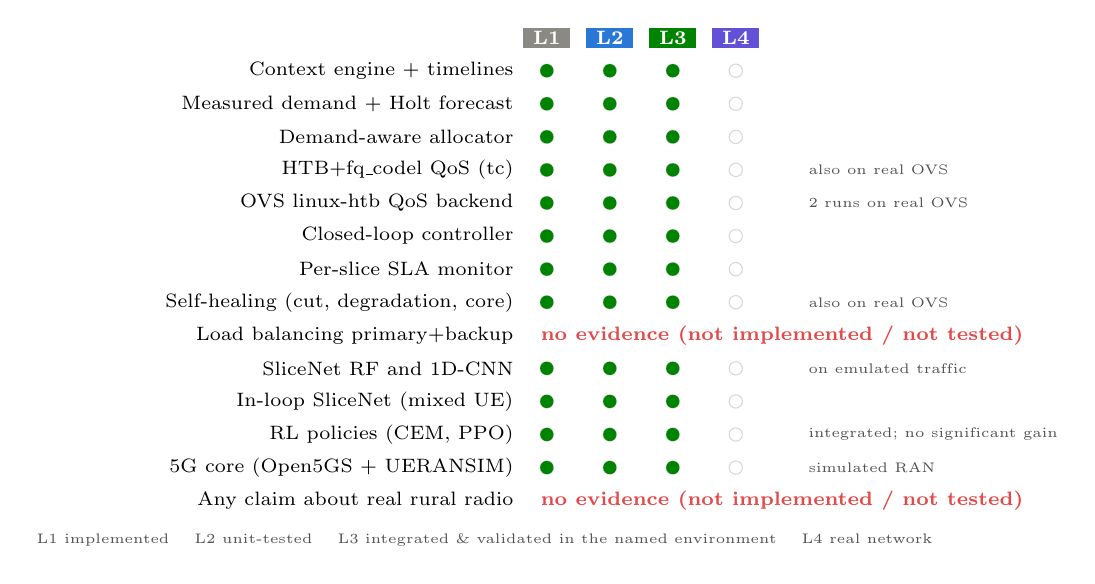
\begin{tikzpicture}[x=1cm,y=0.42cm,font=\scriptsize]
  \foreach \l/\c [count=\i] in {1/lvlone,2/lvltwo,3/lvlthree,4/lvlfour}
    \node[fill=\c,text=white,font=\scriptsize\bfseries,minimum width=6mm,inner sep=1.2pt] at (2.6+0.8*\i,0) {L\l};
  \foreach \name/\lv/\note [count=\r] in {
    {Context engine + timelines}/3/,
    {Measured demand + Holt forecast}/3/,
    {Demand-aware allocator}/3/,
    {HTB+fq\_codel QoS (tc)}/3/also on real OVS,
    {OVS linux-htb QoS backend}/3/2 runs on real OVS,
    {Closed-loop controller}/3/,
    {Per-slice SLA monitor}/3/,
    {Self-healing (cut, degradation, core)}/3/also on real OVS,
    {Load balancing primary+backup}/0/,
    {SliceNet RF and 1D-CNN}/3/on emulated traffic,
    {In-loop SliceNet (mixed UE)}/3/,
    {RL policies (CEM, PPO)}/3/integrated; no significant gain,
    {5G core (Open5GS + UERANSIM)}/3/simulated RAN,
    {Any claim about real rural radio}/0/}{
    \node[anchor=east] at (3.1,-\r) {\name};
    \ifnum\lv>0
      \foreach \k in {1,...,4}{\draw[rule] (2.6+0.8*\k,-\r) circle (2.4pt);}
      \foreach \k in {1,...,\lv}{\fill[lvlthree] (2.6+0.8*\k,-\r) circle (2.4pt);}
    \else
      \node[anchor=west,text=lvlno,font=\scriptsize\bfseries] at (3.2,-\r) {no evidence (not implemented / not tested)};
    \fi
    \node[anchor=west,text=ink2,font=\tiny] at (6.6,-\r) {\note};
  }
  \node[anchor=west,text=ink2,font=\tiny] at (-3.2,-15.2) {L1 implemented \quad L2 unit-tested \quad L3 integrated \& validated in the named environment \quad L4 real network};
\end{tikzpicture}
\caption{Evidence maturity per component. Nothing reaches L4: every network result comes from emulation
(Mininet with Linux bridges or a real Open vSwitch), or from the Open5GS 5G core with a simulated RAN.}
\label{fig:ladder}
\end{figure}}

% ------------------------------------------------------------ architecture
\newcommand{\FigArch}{%
\begin{figure}[!htbp]\centering
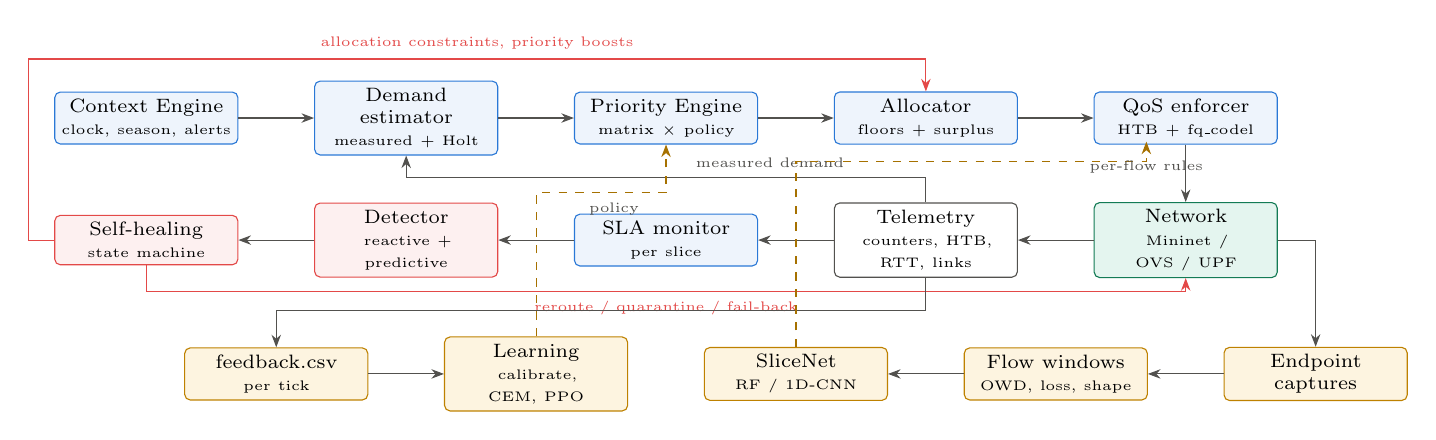
\begin{tikzpicture}[font=\scriptsize,every node/.append style={text width=2.15cm,minimum width=2.3cm}]
  % row 0: live decision path
  \node[live] (ctx) at (0,0) {Context Engine\\\tiny clock, season, alerts};
  \node[live] (dem) at (3.3,0) {Demand estimator\\\tiny measured + Holt};
  \node[live] (pri) at (6.6,0) {Priority Engine\\\tiny matrix $\times$ policy};
  \node[live] (alc) at (9.9,0) {Allocator\\\tiny floors + surplus};
  \node[live] (qos) at (13.2,0) {QoS enforcer\\\tiny HTB + fq\_codel};
  % row 1: network, telemetry, monitoring, healing
  \node[heal] (hea) at (0,-1.55) {Self-healing\\\tiny state machine};
  \node[heal] (det) at (3.3,-1.55) {Detector\\\tiny reactive + predictive};
  \node[live] (mon) at (6.6,-1.55) {SLA monitor\\\tiny per slice};
  \node[mod]  (tel) at (9.9,-1.55) {Telemetry\\\tiny counters, HTB, RTT, links};
  \node[net]  (net) at (13.2,-1.55) {Network\\\tiny Mininet / OVS / UPF};
  % row 2: offline
  \node[off] (fb)  at (1.65,-3.25) {feedback.csv\\\tiny per tick};
  \node[off] (lrn) at (4.95,-3.25) {Learning\\\tiny calibrate, CEM, PPO};
  \node[off] (sn)  at (8.25,-3.25) {SliceNet\\\tiny RF / 1D-CNN};
  \node[off] (fea) at (11.55,-3.25) {Flow windows\\\tiny OWD, loss, shape};
  \node[off] (cap) at (14.85,-3.25) {Endpoint\\captures};
  % live chain
  \draw[arr] (ctx)--(dem); \draw[arr] (dem)--(pri); \draw[arr] (pri)--(alc); \draw[arr] (alc)--(qos);
  \draw[arr] (qos)--(net);
  \draw[arr] (net)--(tel); \draw[arr] (tel)--(mon); \draw[arr] (mon)--(det); \draw[arr] (det)--(hea);
  % feedback paths
  \draw[arr] (tel.north) -- (9.9,-0.75) -| node[lbl,above,pos=0.15,text width=]{measured demand} (dem.south);
  \draw[arr,cH] (hea.west) -- (-1.5,-1.55) -- (-1.5,0.75) -| node[lbl,above,pos=0.25,text width=,text=cH]{allocation constraints, priority boosts} (alc.north);
  \draw[arr,cH] (hea.south) -- (0,-2.2) -| node[lbl,below,pos=0.25,text width=,text=cH]{reroute / quarantine / fail-back} (net.south);
  \draw[arr] (net.east) -| (cap.north);
  \draw[arr] (cap)--(fea); \draw[arr] (fea)--(sn);
  \draw[arr] (tel.south) -- (9.9,-2.45) -| (fb.north);
  \draw[arr] (fb)--(lrn);
  \draw[darr,cD!70!black] (lrn.north) -- (4.95,-0.95) -| node[lbl,below,pos=0.3,text width=]{policy} (pri.south);
  \draw[darr,cD!70!black] (sn.north) -- (8.25,-0.55) -| node[lbl,below,pos=0.75,text width=]{per-flow rules} (12.7,-0.3);
\end{tikzpicture}
\caption{End-to-end architecture. Row 1: live decision path (1\,s ticks, re-plan every 5\,s). Row 2: observation and self-healing.
Row 3: offline data, training and analysis; dashed arrows are artefacts deployed back into the loop.}
\label{fig:arch}
\end{figure}}

% ------------------------------------------------------------ topology
\newcommand{\FigTopo}{%
\begin{figure}[!htbp]\centering
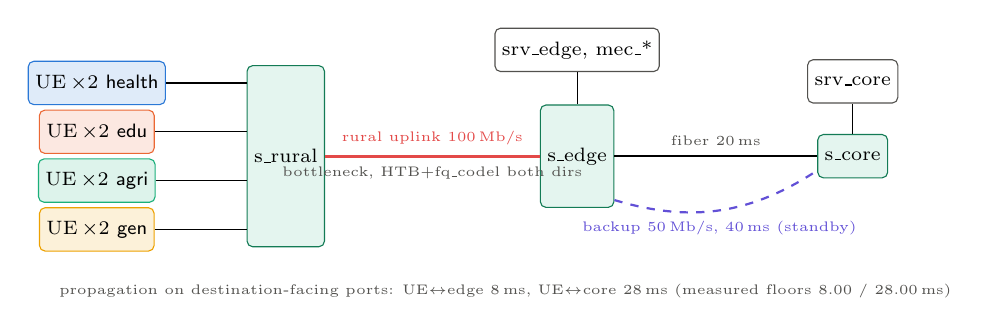
\begin{tikzpicture}[font=\scriptsize,node distance=4mm]
  \foreach \s/\c [count=\i] in {health/cA,edu/cB,agri/cC,gen/cD}{
    \node[mod,fill=\c!15,draw=\c] (u\i) at (0,1.9-0.62*\i) {UE\,$\times$2 \textsf{\s}};}
  \node[net,minimum height=2.3cm] (sr) at (2.4,0.35) {s\_rural};
  \node[net,minimum height=1.3cm] (se) at (6.1,0.35) {s\_edge};
  \node[net] (sc) at (9.6,0.35) {s\_core};
  \node[mod] (srv) at (6.1,1.7) {srv\_edge, mec\_*};
  \node[mod] (core) at (9.6,1.3) {srv\_core};
  \foreach \i in {1,...,4}\draw (u\i.east)--(sr.west|-u\i.east);
  \draw[very thick,cH] (sr.east)--node[above,lbl,text=cH]{rural uplink 100\,Mb/s}node[below,lbl]{bottleneck, HTB+fq\_codel both dirs}(se.west);
  \draw[thick] (se.east)--node[above,lbl]{fiber 20\,ms}(sc.west);
  \draw[dashed,thick,cG] ($(se.south east)+(0,0.1)$) to[bend right=25] node[below,lbl,text=cG]{backup 50\,Mb/s, 40\,ms (standby)} ($(sc.south west)+(0,0.1)$);
  \draw (se)--(srv); \draw (sc)--(core);
  \node[lbl,align=left,anchor=north west] at (-0.6,-1.15) {propagation on destination-facing ports: UE$\leftrightarrow$edge 8\,ms, UE$\leftrightarrow$core 28\,ms (measured floors \NFloorEdge{} / \NFloorCore{}\,ms)};
\end{tikzpicture}
\caption{Emulated rural network: one shared contention point, a primary and a standby backhaul.}
\label{fig:topo}
\end{figure}}

% ------------------------------------------------------------ control-loop tick
\newcommand{\FigTick}{%
\begin{figure}[!htbp]\centering
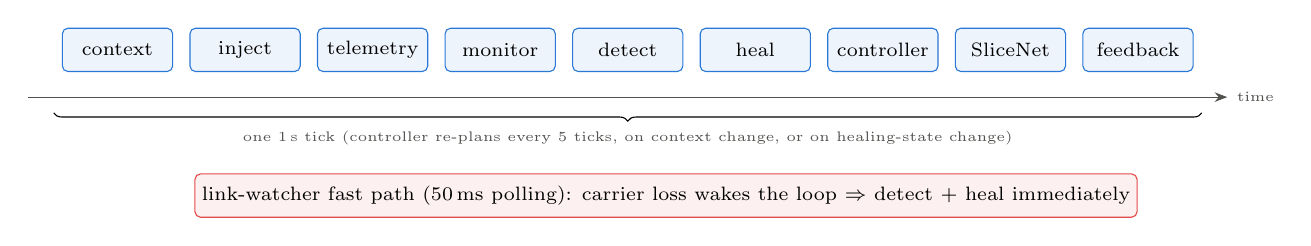
\begin{tikzpicture}[font=\scriptsize,x=1.62cm]
  \draw[arr] (0,0)--(9.4,0) node[right,lbl]{time};
  \foreach \x/\t in {0.2/context,1.2/inject,2.2/telemetry,3.2/monitor,4.2/detect,5.2/heal,6.2/controller,7.2/SliceNet,8.2/feedback}{
     \node[live,minimum width=1.4cm] at (\x+0.5,0.6) {\t};}
  \draw[decorate,decoration={brace,mirror,amplitude=3pt}] (0.2,-0.2)--(9.2,-0.2) node[midway,below=3pt,lbl]{one 1\,s tick (controller re-plans every 5 ticks, on context change, or on healing-state change)};
  \node[heal,align=center] at (5.0,-1.25) {link-watcher fast path (50\,ms polling): carrier loss wakes the loop $\Rightarrow$ detect + heal immediately};
\end{tikzpicture}
\caption{Order of operations per tick (\capcode{core/orchestrator.py}).}
\label{fig:tick}
\end{figure}}

% ------------------------------------------------------------ self-healing state machine
\newcommand{\FigHeal}{%
\begin{figure}[!htbp]\centering
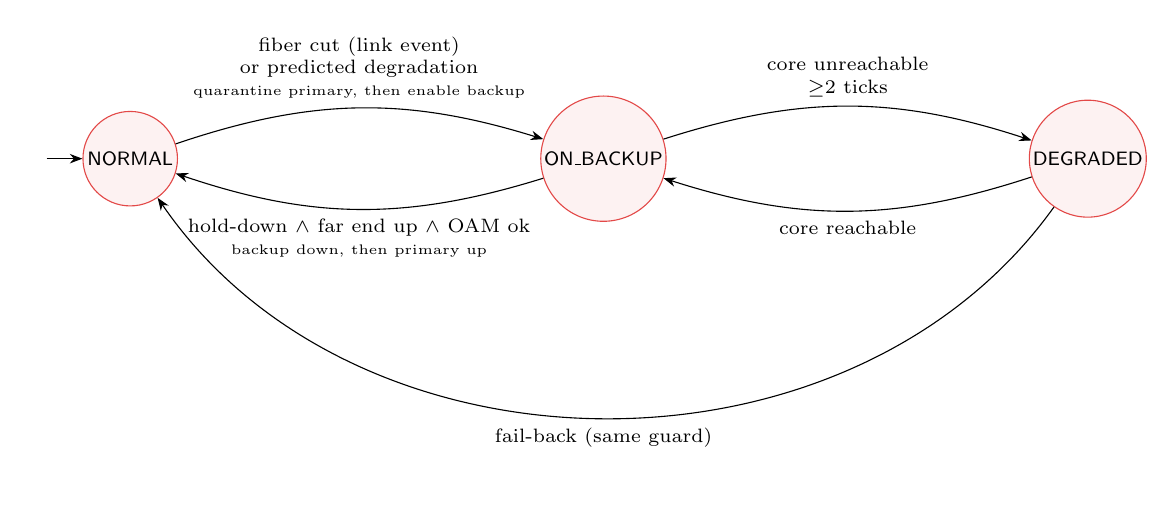
\begin{tikzpicture}[->,>={Stealth[length=1.6mm]},node distance=4.6cm,font=\scriptsize,
   every state/.style={draw=cH,fill=cH!7,minimum size=12mm,inner sep=1pt}]
  \node[state,initial,initial text=] (n) {\textsf{NORMAL}};
  \node[state,right=of n] (b) {\textsf{ON\_BACKUP}};
  \node[state,right=of b] (d) {\textsf{DEGRADED}};
  \path (n) edge[bend left=18] node[above,align=center]{fiber cut (link event)\\or predicted degradation\\\tiny quarantine primary, then enable backup} (b)
        (b) edge[bend left=18] node[below,align=center]{hold-down $\wedge$ far end up $\wedge$ OAM ok\\\tiny backup down, then primary up} (n)
        (b) edge[bend left=18] node[above,align=center]{core unreachable\\$\geq$2 ticks} (d)
        (d) edge[bend left=18] node[below]{core reachable} (b)
        (d) edge[bend left=55] node[below]{fail-back (same guard)} (n);
\end{tikzpicture}
\caption{Self-healing state machine (\capcode{self_healing/engine.py}). The L2 domain is loop-free at every instant.}
\label{fig:heal}
\end{figure}}

% ------------------------------------------------------------ measurement method
\newcommand{\FigMeasure}{%
\begin{figure}[!htbp]\centering
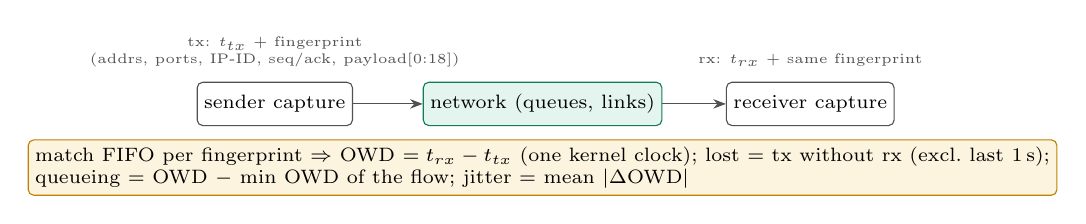
\begin{tikzpicture}[font=\scriptsize]
  \node[mod] (s) at (0,0) {sender capture};
  \node[net] (n) at (3.4,0) {network (queues, links)};
  \node[mod] (r) at (6.8,0) {receiver capture};
  \draw[arr] (s)--(n); \draw[arr] (n)--(r);
  \node[lbl,align=center,anchor=south] at (0,0.35) {tx: $t_{tx}$ + fingerprint\\(addrs, ports, IP-ID, seq/ack, payload[0:18])};
  \node[lbl,align=center,anchor=south] at (6.8,0.35) {rx: $t_{rx}$ + same fingerprint};
  \node[off,align=left,anchor=north] at (3.4,-0.45) {match FIFO per fingerprint $\Rightarrow$ OWD $=t_{rx}-t_{tx}$ (one kernel clock);
    lost $=$ tx without rx (excl.\ last 1\,s);\\ queueing $=$ OWD $-$ min OWD of the flow; jitter $=$ mean $|\Delta$OWD$|$};
\end{tikzpicture}
\caption{Packet-matched one-way delay and loss (\capcode{features/packet_capture.py}).}
\label{fig:measure}
\end{figure}}

% ------------------------------------------------------------ allocation example
\newcommand{\FigAlloc}{%
\begin{figure}[!htbp]\centering
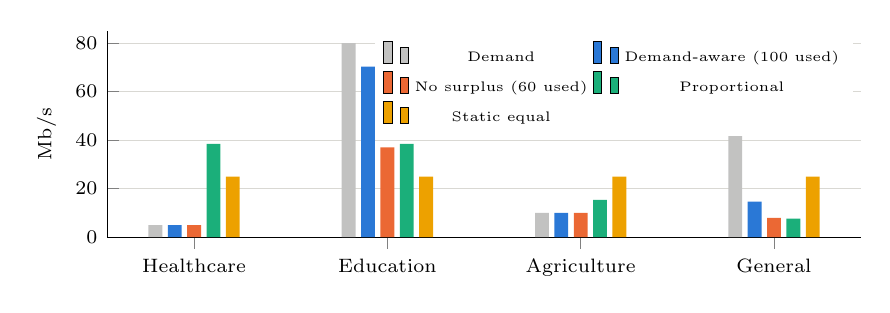
\begin{tikzpicture}
\begin{axis}[ybar,bar width=5pt,width=0.92\linewidth,height=4.2cm,ymin=0,ymax=85,
  symbolic x coords={Healthcare,Education,Agriculture,General},xtick=data,
  ylabel={Mb/s},ylabel style={font=\scriptsize},tick label style={font=\scriptsize},
  legend style={font=\tiny,draw=none,at={(0.99,0.98)},anchor=north east,legend columns=2},
  axis lines*=left,ymajorgrids,grid style={rule},enlarge x limits=0.15]
 \addplot[fill=ink2!35,draw=none] coordinates {(Healthcare,5)(Education,80)(Agriculture,10)(General,50)};
 \addplot[fill=cA,draw=none] coordinates {(Healthcare,5)(Education,70.33)(Agriculture,10)(General,14.67)};
 \addplot[fill=cB,draw=none] coordinates {(Healthcare,5)(Education,37)(Agriculture,10)(General,8)};
 \addplot[fill=cC,draw=none] coordinates {(Healthcare,38.46)(Education,38.46)(Agriculture,15.38)(General,7.69)};
 \addplot[fill=cD,draw=none] coordinates {(Healthcare,25)(Education,25)(Agriculture,25)(General,25)};
 \legend{Demand,Demand-aware (100 used),No surplus (60 used),Proportional,Static equal}
\end{axis}
\end{tikzpicture}
\caption{Allocators on the school context (demand 145\,Mb/s on 100\,Mb/s; weights 5/5/2/1; floors 5/2/1/1).
Values are produced by \capcode{slicing/allocators.py}.}
\label{fig:alloc}
\end{figure}}

% ------------------------------------------------------------ SliceNet pipeline
\newcommand{\FigSliceNet}{%
\begin{figure}[!htbp]\centering
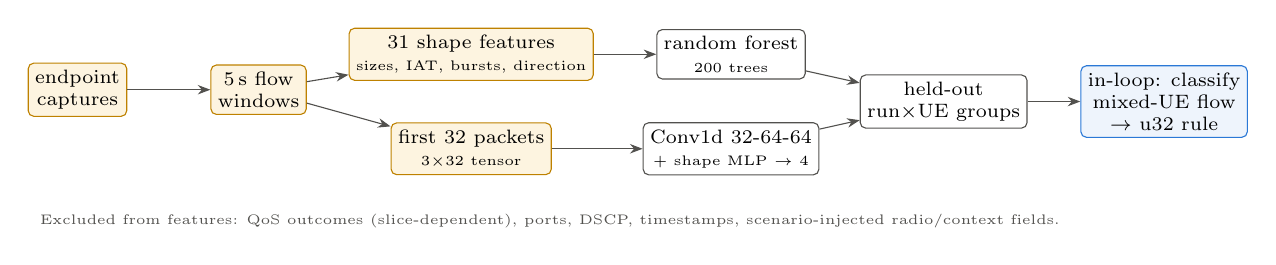
\begin{tikzpicture}[font=\scriptsize]
  \node[off] (cap) at (0,0) {endpoint\\captures};
  \node[off] (win) at (2.3,0) {5\,s flow\\windows};
  \node[off] (shape) at (5.0,0.45) {31 shape features\\\tiny sizes, IAT, bursts, direction};
  \node[off] (seq) at (5.0,-0.75) {first 32 packets\\\tiny 3$\times$32 tensor};
  \node[mod] (rf) at (8.3,0.45) {random forest\\\tiny 200 trees};
  \node[mod] (cnn) at (8.3,-0.75) {Conv1d 32-64-64\\\tiny + shape MLP $\rightarrow$ 4};
  \node[mod] (gs) at (11.0,-0.15) {held-out\\run$\times$UE groups};
  \node[live] (inl) at (13.8,-0.15) {in-loop: classify\\mixed-UE flow\\$\rightarrow$ u32 rule};
  \draw[arr] (cap)--(win); \draw[arr] (win)--(shape); \draw[arr] (win)--(seq);
  \draw[arr] (shape)--(rf); \draw[arr] (seq)--(cnn); \draw[arr] (rf)--(gs); \draw[arr] (cnn)--(gs); \draw[arr] (gs)--(inl);
  \node[lbl,anchor=north west] at (-0.6,-1.45) {Excluded from features: QoS outcomes (slice-dependent), ports, DSCP, timestamps, scenario-injected radio/context fields.};
\end{tikzpicture}
\caption{SliceNet: features, models, evaluation protocol and in-loop use.}
\label{fig:slicenet}
\end{figure}}

% ------------------------------------------------------------ 5G deployment
\newcommand{\FigFiveG}{%
\begin{figure}[!htbp]\centering
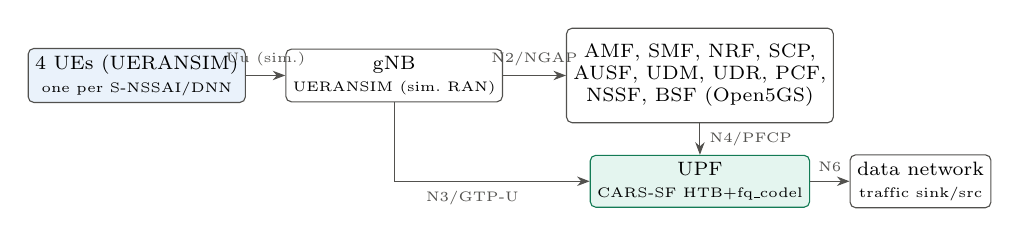
\begin{tikzpicture}[font=\scriptsize,node distance=4mm and 5mm]
  \node[mod,fill=cA!10] (ue) {4 UEs (UERANSIM)\\\tiny one per S-NSSAI/DNN};
  \node[mod,right=of ue] (gnb) {gNB\\\tiny UERANSIM (sim.\ RAN)};
  \node[mod,right=8mm of gnb,minimum width=2.6cm,minimum height=1.2cm] (cp) {AMF, SMF, NRF, SCP,\\AUSF, UDM, UDR, PCF,\\NSSF, BSF (Open5GS)};
  \node[net,below=of cp] (upf) {UPF\\\tiny CARS-SF HTB+fq\_codel};
  \node[mod,right=of upf] (dn) {data network\\\tiny traffic sink/src};
  \draw[arr] (ue)--node[above,lbl]{Uu (sim.)}(gnb);
  \draw[arr] (gnb)--node[above,lbl]{N2/NGAP}(cp);
  \draw[arr] (gnb.south) |- node[below,lbl,pos=0.7]{N3/GTP-U} (upf);
  \draw[arr] (cp)--node[right,lbl]{N4/PFCP}(upf);
  \draw[arr] (upf)--node[above,lbl]{N6}(dn);
\end{tikzpicture}
\caption{Real 5G core deployment (\capcode{deployment/5g}). CARS-SF enforces at the UPF, classifying by slice address pool.}
\label{fig:fiveg}
\end{figure}}

% ------------------------------------------------------------ results: healthcare SLA share
\newcommand{\FigMainSla}{%
\begin{figure}[!htbp]\centering
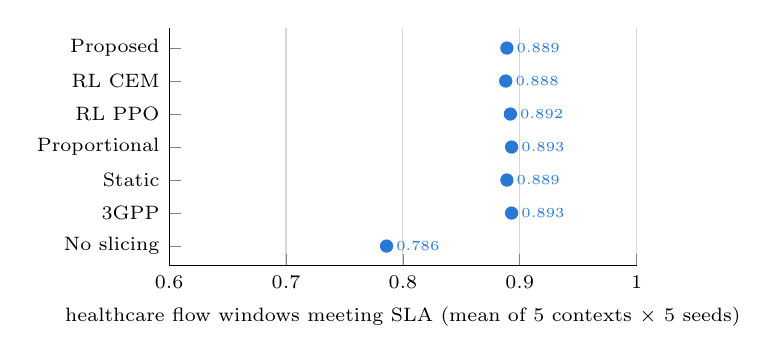
\begin{tikzpicture}
\begin{axis}[width=0.62\linewidth,height=4.6cm,xmin=0.6,xmax=1,
  symbolic y coords={No slicing,3GPP,Static,Proportional,RL PPO,RL CEM,Proposed},ytick=data,
  xlabel={healthcare flow windows meeting SLA (mean of 5 contexts $\times$ 5 seeds)},
  xlabel style={font=\scriptsize},tick label style={font=\scriptsize},axis lines*=left,xmajorgrids,grid style={rule},
  nodes near coords,nodes near coords style={font=\tiny,anchor=west},point meta=explicit symbolic]
 \addplot[only marks,mark=*,mark size=2.2pt,cA] coordinates {(\NHcSlaNoSlicing,No slicing)[\NHcSlaNoSlicing](\NHcSlaTgpp,3GPP)[\NHcSlaTgpp](\NHcSlaStatic,Static)[\NHcSlaStatic](\NHcSlaProportional,Proportional)[\NHcSlaProportional](\NHcSlaPpo,RL PPO)[\NHcSlaPpo](\NHcSlaCem,RL CEM)[\NHcSlaCem](\NHcSlaProposed,Proposed)[\NHcSlaProposed]};
\end{axis}
\end{tikzpicture}
\caption{Any slicing vs none: the significant effect in the main study
($\Delta=\NSlaDeltaNoSlicing$, Wilcoxon $p=\NSlaPNoSlicing$, $n=\NSlaPairs$ pairs).
The differences between slicing schemes are not significant. Dots, not bars: the axis is zoomed to 0.6--1.}
\label{fig:mainsla}
\end{figure}}

% ------------------------------------------------------------ results: ablation
\newcommand{\FigAblation}{%
\begin{figure}[!htbp]\centering
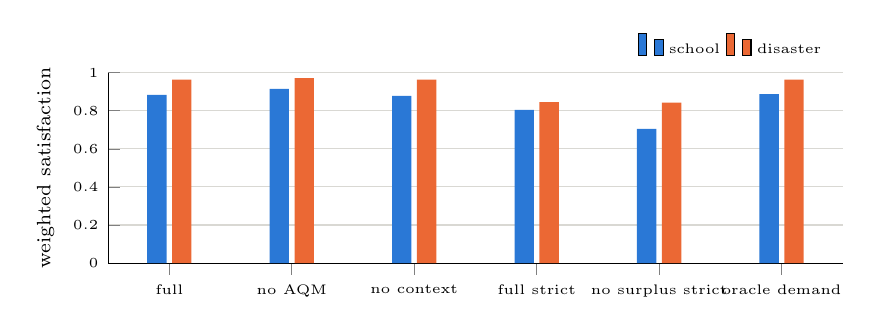
\begin{tikzpicture}
\begin{axis}[ybar,bar width=7pt,width=0.9\linewidth,height=4cm,ymin=0,ymax=1,
  symbolic x coords={full,no AQM,no context,full strict,no surplus strict,oracle demand},xtick=data,
  ylabel={weighted satisfaction},ylabel style={font=\scriptsize},tick label style={font=\tiny},
  legend style={font=\tiny,draw=none,at={(0.99,1.02)},anchor=south east,legend columns=2},axis lines*=left,ymajorgrids,grid style={rule}]
 \addplot[fill=cA,draw=none] coordinates {(full,\NAblSchoolFullUtil)(no AQM,\NAblSchoolNoAqmUtil)(no context,\NAblSchoolNoContextUtil)(full strict,\NAblSchoolFullStrictUtil)(no surplus strict,\NAblSchoolNoSurplusStrictUtil)(oracle demand,\NAblSchoolOracleDemandUtil)};
 \addplot[fill=cB,draw=none] coordinates {(full,\NAblDisasterFullUtil)(no AQM,\NAblDisasterNoAqmUtil)(no context,\NAblDisasterNoContextUtil)(full strict,\NAblDisasterFullStrictUtil)(no surplus strict,\NAblDisasterNoSurplusStrictUtil)(oracle demand,\NAblDisasterOracleDemandUtil)};
 \legend{school,disaster}
\end{axis}
\end{tikzpicture}
\caption{Ablation (3 seeds). Strict caps (no borrowing) cost the most; surplus redistribution matters only once borrowing is disabled.
Removing AQM \emph{raises} this throughput metric while tail delay explodes (Q463); removing context changes nothing measurable.}
\label{fig:ablation}
\end{figure}}

% ------------------------------------------------------------ results: resilience
\newcommand{\FigResilience}{%
\begin{figure}[!htbp]\centering
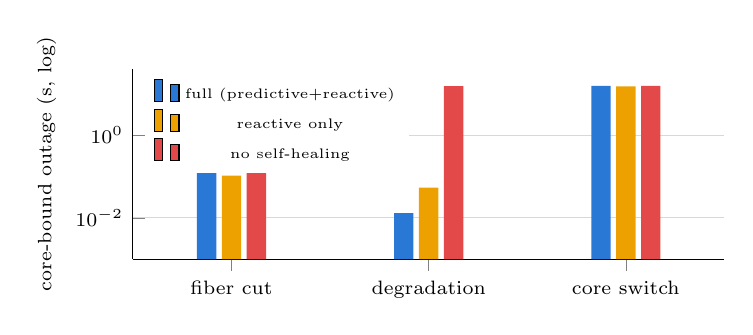
\begin{tikzpicture}
\begin{axis}[ybar,bar width=7pt,width=0.75\linewidth,height=4cm,ymode=log,ymin=0.001,ymax=40,log origin=infty,
  symbolic x coords={fiber cut,degradation,core switch},xtick=data,
  ylabel={core-bound outage (s, log)},ylabel style={font=\scriptsize},tick label style={font=\scriptsize},
  legend style={font=\tiny,draw=none,at={(0.02,0.98)},anchor=north west},axis lines*=left,ymajorgrids,grid style={rule},enlarge x limits=0.25]
 \addplot[fill=cA,draw=none] coordinates {(fiber cut,\NOutCutFullMean)(degradation,\NOutDegFullMean)(core switch,\NOutCoreFullMean)};
 \addplot[fill=cD,draw=none] coordinates {(fiber cut,\NOutCutReactiveMean)(degradation,\NOutDegReactiveMean)(core switch,\NOutCoreReactiveMean)};
 \addplot[fill=cH,draw=none] coordinates {(fiber cut,\NOutCutNoneMean)(degradation,\NOutDegNoneMean)(core switch,\NOutCoreNoneMean)};
 \legend{full (predictive+reactive),reactive only,no self-healing}
\end{axis}
\end{tikzpicture}
\caption{Longest delivery gap of core-bound flows after the failure (packet-matched, 3 seeds; log scale).
Core-switch failure cannot be bypassed: healing localises the fault but cannot restore core-hosted services.}
\label{fig:resilience}
\end{figure}}

% ------------------------------------------------------------ results: transfer
\newcommand{\FigTransfer}{%
\begin{figure}[!htbp]\centering
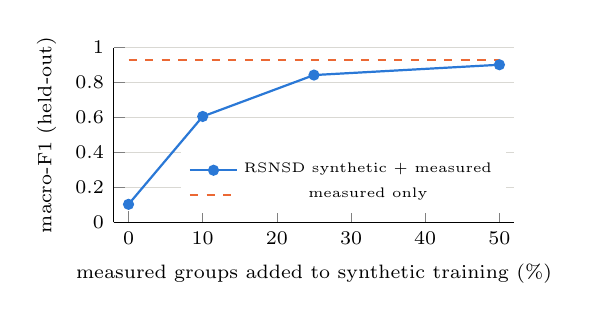
\begin{tikzpicture}
\begin{axis}[width=0.55\linewidth,height=3.8cm,xmin=-2,xmax=52,ymin=0,ymax=1,
  xlabel={measured groups added to synthetic training (\%)},ylabel={macro-F1 (held-out)},
  label style={font=\scriptsize},tick label style={font=\scriptsize},axis lines*=left,ymajorgrids,grid style={rule},
  legend style={font=\tiny,draw=none,at={(0.98,0.05)},anchor=south east}]
 \addplot[cA,thick,mark=*,mark size=1.6pt] coordinates {(0,\NTrZero)(10,\NTrTen)(25,\NTrQuarter)(50,\NTrHalf)};
 \addplot[cB,dashed,thick,domain=0:50] {\NTrMininetOnly};
 \legend{RSNSD synthetic + measured,measured only}
\end{axis}
\end{tikzpicture}
\caption{Synthetic-to-measured transfer: RSNSD alone is near chance on measured traffic.}
\label{fig:transfer}
\end{figure}}

% ------------------------------------------------------------ results: load sensitivity
\newcommand{\FigLoad}{%
\begin{figure}[!htbp]\centering
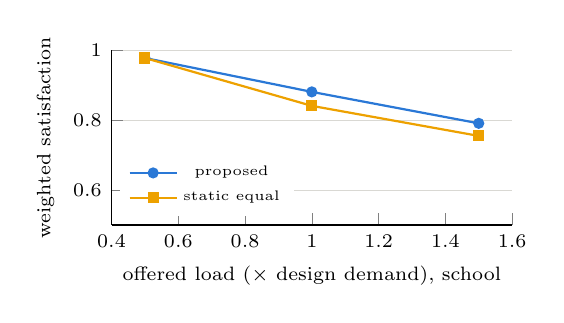
\begin{tikzpicture}
\begin{axis}[width=0.55\linewidth,height=3.8cm,xmin=0.4,xmax=1.6,ymin=0.5,ymax=1,
  xlabel={offered load ($\times$ design demand), school},ylabel={weighted satisfaction},
  label style={font=\scriptsize},tick label style={font=\scriptsize},axis lines*=left,ymajorgrids,grid style={rule},
  legend style={font=\tiny,draw=none,at={(0.02,0.05)},anchor=south west}]
 \addplot[cA,thick,mark=*,mark size=1.6pt] coordinates {(0.5,\NSensLoadSchoolProposedZeropFive)(1,\NSensLoadSchoolProposedOne)(1.5,\NSensLoadSchoolProposedOnepFive)};
 \addplot[cD,thick,mark=square*,mark size=1.6pt] coordinates {(0.5,\NSensLoadSchoolStaticZeropFive)(1,\NSensLoadSchoolStaticOne)(1.5,\NSensLoadSchoolStaticOnepFive)};
 \legend{proposed,static equal}
\end{axis}
\end{tikzpicture}
\caption{Load sensitivity (school, 3 seeds): the proposed scheduler helps only once demand exceeds capacity.}
\label{fig:load}
\end{figure}}


\title{\vspace{-1.2cm}\textbf{CARS-SF}\\[2pt]\large Design-Defense Handbook for the RPAC and Thesis Panel\\[2pt]
\normalsize Context-Aware Rural Service Slicing Framework with autonomous self-healing}
\author{Prepared for the thesis presenter}
\date{October 2026 \textperiodcentered{} numbers generated from \code{results/} by \code{experiments/defense_numbers.py}}

\begin{document}
\maketitle
\thispagestyle{empty}

\begin{keybox}{How to use this handbook}
Every design question is answered in five parts:
\textbf{Why} (the requirement), \textbf{Choice} (what was built), \textbf{Alternative} (what else was possible),
\textbf{Trade-off} (what was gained and given up) and \textbf{Evidence}. Each piece of evidence carries a
\emph{maturity badge}. The four levels are different kinds of evidence, never interchangeable:\\[2pt]
\Lone{} the code exists \quad \Ltwo{} isolated tests pass \quad
\Lthree{} works with the real connected components \emph{in the stated environment} \quad
\Lfour{} tested on real infrastructure.\\[2pt]
\textbf{No CARS-SF claim is at L4.} The strongest evidence is L3, and the environment is always named:
Mininet with Linux bridges (sudo-free harness), Mininet with a real Open vSwitch (privileged container), or
the Open5GS 5G core with a UERANSIM-simulated RAN. When an examiner asks ``does it work?'', answer with the
level and the environment, never just ``yes''.\\[2pt]
\textcolor{cH}{\textbf{Honest limit}} marks a weakness to volunteer before it is found; \textbf{If pressed} gives a fallback line for hostile follow-ups.
All numbers are macros generated from the result tables, so they cannot drift from the data.
\end{keybox}

\FigLadder

\begin{keybox}{The ten numbers to know cold}
\begin{enumerate}[leftmargin=1.4em]
\item \NRuns{} emulated runs (\NRunsMain{} in the main study), all with packet-matched measurements; median validation score \NValidationMedian/100.
\item Main study: weighted satisfaction lies between \NUtilMin{} and \NUtilMax{} across all seven schedulers.
  \textbf{No allocation policy is significantly better} after Bonferroni correction (smallest $p=\NUtilPMin$).
\item \textbf{Slicing vs none:} healthcare SLA-met share rises by \NSlaDeltaNoSlicing{} ($p=\NSlaPNoSlicing$, $n=\NSlaPairs$, survives Bonferroni). This is an exploratory finding, not a pre-registered hypothesis.
\item Ablation (school): removing HTB borrowing raises healthcare p95 from \NAblSchoolFullHc{} to \NAblSchoolFullStrictHc{}\,ms.
  Surplus redistribution matters only once borrowing is disabled (\NAblSchoolFullStrictUtil{} $\rightarrow$ \NAblSchoolNoSurplusStrictUtil).
  Removing AQM \emph{raises} throughput satisfaction (\NAblSchoolNoAqmUtil) but general-internet p95 explodes (\NAblSchoolFullGenP{} $\rightarrow$ \NAblSchoolNoAqmGenP\,ms). Removing context awareness changes nothing measurable.
\item Fiber cut: core-bound outage averages \NOutCutFullMean\,s with healing vs \NOutCutNoneMean\,s without. On real OVS, recovery takes \NOvsMttrAfter\,s.
\item Backhaul degradation: the predictive detector switched over before the cut in \NDegBeforeCutShare{} of runs (outage \NOutDegFullMean\,s vs \NOutDegReactiveMean\,s reactive-only).
\item SliceNet on measured traffic: RF macro-F1 \NSnRfFone, 1D-CNN \NSnCnnFone, on held-out runs$\times$UEs (\NSnRows{} windows, \NSnRunsCount{} runs).
\item Synthetic RSNSD scores macro-F1 \NTrZero{} zero-shot on measured flows (near chance), \NTrHalf{} with half the measured groups added.
\item RL: PPO vs the rule-based policy differs by $\Delta=\NPpoDelta$ ($p=\NPpoP$). \textbf{No significant gain.}
\item Real 5G core (10\,Mb/s UPF, disaster): healthcare p95 \NFgDisasterCarsHcP\,ms with CARS-SF vs \NFgDisasterNoneHcP\,ms without. No gain in school, where healthcare is uncontended (\NFgSchoolCarsHcP{} vs \NFgSchoolNoneHcP\,ms), so H8 as pre-registered is \textbf{not supported}.
\end{enumerate}
\end{keybox}

\begin{warnbox}{The claims boundary: what the thesis does and does not claim}
\textbf{Claims (L3, emulation):}
\begin{itemize}
\item service-centric slices enforced at a shared rural bottleneck measurably protect critical-service SLAs;
\item the closed loop detects and heals backhaul and core faults without loops, in sub-second time on real OVS;
\item service classes can be recognised from traffic shape and used to slice a multi-service device.
\end{itemize}
\textbf{Does not claim:}
\begin{itemize}
\item radio-layer QoS or any real-deployment performance;
\item that the demand-aware allocator beats simple slicing on average (it does not, significantly);
\item that RL adds value here (it does not);
\item that context awareness itself improves outcomes (the ablation shows no measurable effect);
\item that RSNSD represents real rural traffic (the transfer study says it does not);
\item load balancing across primary and backup (not implemented).
\end{itemize}
\end{warnbox}

\tableofcontents
\clearpage

\part{The problem statement and research motivation}

\section{What exactly is the problem?}

\begin{qa}{1}{Define the CARS-SF problem in one precise sentence.}
When several socially critical services share one scarce, failure-prone rural backhaul, decide continuously how
much of that bottleneck each \emph{service} receives (from the operating context and measured demand), enforce
that decision in the data plane, and restore connectivity on its own when the backhaul degrades or fails, while
keeping critical-service SLAs.
\end{qa}

\begin{qa}{2}{What does CARS-SF stand for, and what does each part of the name mean operationally?}
\textbf{C}ontext-\textbf{A}ware \textbf{R}ural \textbf{S}ervice \textbf{S}licing \textbf{F}ramework.
\begin{itemize}
\item \emph{Context-aware}: the priority matrix is chosen by \code{ContextInferenceEngine} from clock, season, alerts
and admin override (\code{context/engine.py}).
\item \emph{Rural}: one shared uplink is the only contention point, with a standby backup backhaul (Fig.~\ref{fig:topo}).
\item \emph{Service slicing}: four classes (healthcare, education, agriculture, general), each with its own HTB class,
floor and SLA (\code{registries/slices.yaml}), not eMBB/URLLC/mMTC.
\item \emph{Framework}: swappable stages behind protocols (\code{core/interfaces.py}), composed from
\code{registries/schedulers.yaml}.
\end{itemize}
The thesis title also says ``autonomous self-healing'': the \code{SelfHealingEngine}.
\end{qa}

\begin{qa}{3}{Is the primary research problem rural connectivity, service-aware allocation, context awareness, slicing, self-healing, or their integration?}
The integration: a single closed loop in which context, measured demand, service slicing and self-healing act on
the \emph{same} bottleneck through shared constraints. The healer constrains the allocator rather than overwriting it
(\code{apply_constraints}). Rural connectivity is the setting, not the contribution.
\honest{Integration is a weaker novelty claim than a new algorithm. Defend it with what integration
\emph{enabled} that the parts alone cannot: backup-capacity ceilings that prevent bufferbloat after failover, and
congestion-aware prediction that prevents false failover (both found and fixed in this work).}
\end{qa}

\begin{qa}{4}{Which is the central contribution, and which are supporting engineering components?}
\textbf{Central:}
\begin{itemize}
\item (C1) service-centric slicing with a context-driven, demand-aware allocator enforced at the rural bottleneck;
\item (C2) a loop-free self-healing state machine with predictive switchover, integrated with allocation;
\item (C3) a packet-matched measurement methodology that makes C1 and C2 evaluable.
\end{itemize}
\textbf{Supporting:} traffic models, harness, matrix runner, 5G deployment.
\textbf{Secondary research results:} SliceNet on measured traffic and the synthetic-to-measured transfer study.
RL is an evaluated alternative with a \emph{negative} result.
\end{qa}

\begin{qa}{5}{What concrete failure or inefficiency exists in a conventional rural network that CARS-SF addresses?}
\begin{itemize}
\item (a) A single FIFO uplink lets bulk downloads and video inflate everyone's queue. In the main study, ``no slicing''
meets the healthcare SLA in \NHcSlaNoSlicing{} of windows vs \NHcSlaProposed{} with slicing.
\item (b) Static per-technology shares (3GPP-style) ignore that a disaster changes \emph{which} service matters.
\item (c) A fiber cut with no automated failover means an outage of the order of the repair time. Without self-healing,
the injected cut cost \NOutCutNoneMean\,s of core-bound outage in each run (until the scripted repair).
\end{itemize}
\end{qa}

\begin{qa}{6}{What do you mean by resilient connectivity? Which measurable properties constitute resilience?}
Six measured properties:
\begin{itemize}
\item time to detect (MTTD) and time to act (control-plane MTTR);
\item service outage: the longest delivery gap of affected flows, from matched packets;
\item packets lost during failover;
\item SLA compliance while degraded;
\item correct localisation (link vs core switch);
\item safe fail-back with no loops or flapping.
\end{itemize}
All six are produced per run (\code{healer.resilience_summary}, \code{analysis/metrics.outage_metrics}).
Availability over months is \emph{not} measured.
\end{qa}

\begin{qa}{7}{What do you mean by context-aware? What qualifies as context, and how does it change a decision?}
Context is information \emph{external} to the traffic that changes social priority:
\begin{itemize}
\item time of day and weekday (school hours);
\item season (harvest months);
\item alerts (flood, fire, medical emergency, fiber cut);
\item an administrative override.
\end{itemize}
It selects the priority matrix (e.g.\ disaster: healthcare weight 10 vs 1), and in timeline runs it also changes the
offered traffic. It does \emph{not} change floors or SLA targets.
\ev{timeline runs switch contexts live; unit tests check the precedence rules (\code{tests/test_context.py}).}{\Lthree}
\end{qa}

\begin{qa}{8}{What do you mean by self-healing? How does it differ from detecting a fault, raising an alert or manual repair?}
Self-healing closes the loop: it detects (link watcher, telemetry, prediction), diagnoses (link vs core switch),
acts on the network (quarantine, backup activation, MAC flush), adapts the allocation (constraints, ceilings), and
reverts safely once the fault has cleared (hold-down + OAM check). An alert stops at detection; manual repair needs a human.
\honest{Post-action verification is partial. Escalation to \textsf{DEGRADED} happens when the core is still unreachable
after failover, but there is no generic ``verify KPI, otherwise roll back'' stage for every action (see Q514).}
\end{qa}

\begin{qa}{9}{What is the exact system boundary of CARS-SF?}
\textbf{Inside:}
\begin{itemize}
\item the control loop (\code{core/}, \code{slicing/}, \code{self_healing/}, \code{scheduler/}, \code{classification/online.py});
\item the qdiscs and filters on the two ends of the rural uplink;
\item the s\_edge-side backhaul ports.
\end{itemize}
\textbf{Outside:}
\begin{itemize}
\item end hosts and their congestion control;
\item the core and edge servers;
\item the radio access network;
\item physical repair.
\end{itemize}
The traffic generators, topology and capture are \emph{experimental apparatus}, not part of the framework.
\end{qa}

\begin{qa}{10}{What does CARS-SF control, what does it observe, and what is outside its control?}
\textbf{Controls:}
\begin{itemize}
\item HTB rates and ceilings per class, in both directions;
\item classification rules (host, app, per-flow);
\item the admin state of the s\_edge backhaul and backup ports;
\item the forwarding database (MAC flush).
\end{itemize}
\textbf{Observes:}
\begin{itemize}
\item interface counters and HTB class stats;
\item RTT probes and link state;
\item OVS stats (on OVS);
\item packet captures (post-run, plus live for the mixed UE).
\end{itemize}
\textbf{Outside its control:} offered load, TCP behaviour, the far end of the backhaul, the radio.
\end{qa}

\begin{qa}{11}{Is CARS-SF a protocol, a management framework, a decision engine, a dataset, an ML model, or a combination?}
Most defensible: \emph{a network-management framework with a closed-loop decision engine}, plus an evaluation
methodology. It is not a protocol and does not change packet formats. Datasets (RSNSD, the measured windows)
and models (SliceNet, PPO) are \emph{artefacts} it produces and consumes.
\end{qa}

\begin{qa}{12}{What is the unit of decision-making?}
The \textbf{service slice} (four HTB classes) for allocation, re-planned every 5\,s. The \textbf{flow} (5-tuple) only
for in-loop classification of a mixed UE. The \textbf{link} for self-healing. There are no per-packet decisions:
the kernel's HTB and fq\_codel handle packets.
\end{qa}

\begin{qa}{13}{What is the unit of failure detection and recovery?}
Detection: a link (carrier transition on \code{s_edge-bh}), reachability per tier (edge vs core RTT probes), and the
per-slice SLA. Recovery: path-level (primary $\leftrightarrow$ backup backhaul) plus slice-level constraints.
\end{qa}

\begin{qa}{14}{What does the system optimise, and what constraints must never be violated?}
It maximises priority-weighted demand satisfaction
$U=\sum_s w_s\min(1,x_s/d_s)/\sum_s w_s$, approximately and greedily (Q432).
\textbf{Hard constraints:}
\begin{itemize}
\item $\sum_s x_s\le C$;
\item $x_s\ge \min(f_s,d_s)$ for the floors $f$ (healthcare 5, education 2, agriculture 1, general 1\,Mb/s);
\item the L2 domain is never looped;
\item learned policies can only rescale priorities, never bypass floors or constraints.
\end{itemize}
\end{qa}

\begin{qa}{15}{Maximise average performance, or guarantee minimum quality for critical applications?}
Minimum guarantees first: floors are allocated before any priority share, and HTB \code{rate} is a reservation.
Above the floors it maximises weighted satisfaction.
\honest{The floors are bandwidth guarantees, not latency guarantees. Latency is protected empirically
(fq\_codel + priority), not provably (Q461).}
\end{qa}

\begin{qa}{16}{Improving average performance vs preserving critical connectivity in an emergency?}
The average can stay flat while the critical service collapses. In the main study, weighted satisfaction is
statistically indistinguishable across schedulers (\NUtilMin--\NUtilMax), yet healthcare SLA compliance differs by
\NSlaDeltaNoSlicing{} between slicing and no slicing. CARS-SF is judged on the second kind of metric.
\end{qa}

\begin{qa}{17}{Which user-facing outcomes improve if CARS-SF works?}
\begin{itemize}
\item Telemedicine and ECG streams keep low delay and loss under load (healthcare p95 $\approx$\NHcPninefiveProposed\,ms in the main study).
\item Classrooms and downloads get the surplus instead of a fixed share.
\item A fiber cut is a sub-second blip instead of a minutes-long outage.
\item A shared multi-service device (a village kiosk) still gets per-service treatment.
\end{itemize}
\end{qa}

\begin{qa}{18}{What is the smallest implementation that could demonstrate the central hypothesis?}
One bottleneck, two classes (critical vs bulk), HTB+fq\_codel, a static context switch and an injected link cut with a
standby path. Measure the critical SLA and outage with and without. The \code{ablation} and \code{resilience} studies
are essentially this, scaled up.
\end{qa}

\begin{qa}{19}{What functionality is unnecessary for proving that hypothesis?}
RL policies, SliceNet, the 5G deployment, the RSNSD generator, PPO calibration and the OVS QoS backend. They answer
\emph{secondary} questions (RQ3, RQ5, RQ6, RQ8). The thesis presents them as such.
\end{qa}

\begin{qa}{20}{What is explicitly outside the scope of the thesis?}
\begin{itemize}
\item radio scheduling and handover;
\item real field deployment;
\item multi-site topologies with several bottlenecks;
\item multipath load balancing;
\item controller high availability;
\item security of context feeds;
\item energy and power-failure modelling;
\item real-trace traffic.
\end{itemize}
\end{qa}

\section{Why rural networks?}

\begin{qa}{21}{Why rural connectivity rather than generic enterprise networking?}
Rural sites typically combine one scarce shared backhaul, little redundancy, long repair times and a few socially
critical services (clinic, school, farm cooperative) whose importance swings with events (harvest, flood). Enterprise
networks usually have redundant links and overprovisioning, so allocation under scarcity and autonomous healing
matter less there.
\honest{This characterisation is argued from the problem framing and literature, not from rural measurements made
in this thesis.}
\end{qa}

\begin{qa}{22}{Which rural characteristics make the problem technically different?}
\begin{itemize}
\item A single contention point carries every service.
\item Demand composition changes with context more than with load.
\item The backhaul is long and fragile, and any backup has lower capacity.
\item Repair takes long, so autonomy matters.
\end{itemize}
\end{qa}

\begin{qa}{23}{Limited bandwidth, intermittent backhaul, power, sparse infrastructure, latency or poor redundancy?}
Represented: limited bandwidth (100\,Mb/s shared, swept 50--150), backhaul failure and degradation, poor redundancy
(a single standby backup at half capacity), and long backhaul delay (20\,ms primary, 40\,ms backup).
Not represented: power instability, sparse radio coverage.
\end{qa}

\begin{qa}{24}{Which constraints are directly represented in the testbed?}
\begin{itemize}
\item bottleneck capacity (HTB root = 100\,Mb/s);
\item propagation delays (netem on destination-facing ports);
\item a backup path of 50\,Mb/s and 40\,ms;
\item failures: fiber cut, gradual degradation (delay +15\,ms and loss +0.3\% per tick), core switch failure.
\end{itemize}
See \code{topology/rural_topology.py} and \code{self_healing/injector.py}.
\end{qa}

\begin{qa}{25}{Which are only assumed or discussed conceptually?}
Power failures, radio coverage gaps, weather-driven radio degradation, the cost of a backup link, multi-village
topologies and actual rural traffic mixes. The radio fields in RSNSD are scenario-injected and excluded from ML.
\end{qa}

\begin{qa}{26}{What evidence supports heterogeneous, competing requirements of rural services?}
The application registry assigns per-application SLAs (e.g.\ ECG 20\,ms, telemedicine 50\,ms, bulk library 300\,ms,
irrigation 500\,ms) and distinct traffic models.
\honest{These are literature-typical values chosen by design (\code{registries/applications.yaml}), not measured
in rural deployments. The heterogeneity is \emph{assumed} and then modelled.}
\end{qa}

\begin{qa}{27}{Rural network vs low-capacity network: interchangeable in your formulation?}
Not quite. A low-capacity network explains the scarcity. ``Rural'' adds a single fragile backhaul with a weaker backup,
socially prioritised services, and context swings. The allocation results would carry over to any single-bottleneck
network; the resilience results depend on the rural assumptions.
\end{qa}

\begin{qa}{28}{Why not solve it by increasing bandwidth?}
\begin{itemize}
\item Capacity is the expensive, slow resource in rural areas.
\item The capacity sweep (\code{sensitivity_capacity}) shows the proposed scheduler's advantage is modest at every capacity.
At 50\,Mb/s in disaster it protects healthcare better (SLA share \NSensCapDisasterProposedFiveZeroHcSla{} vs
\NSensCapDisasterStaticFiveZeroHcSla), without higher utility.
\item More bandwidth does not fix a cut fiber.
\end{itemize}
\end{qa}

\begin{qa}{29}{Why might adding bandwidth fail for intermittent or physical failures?}
A cut link has zero capacity whatever its nominal size. Recovery needs a \emph{different} path, plus fast
detection and safe switching. Bandwidth helps only the backup's quality while on backup.
\end{qa}

\begin{qa}{30}{No alternate route, no spare capacity, no radio coverage?}
Then CARS-SF can only \emph{degrade gracefully}: it detects the fault, gives the surviving capacity (e.g.\ edge-hosted
services) to critical slices, and reports. This is exactly the core-switch-failure case: the outage of core-hosted
services lasts until repair (\NOutCoreFullMean\,s, the same as without healing), while edge services keep running.
\end{qa}

\begin{qa}{31}{Can software restore connectivity when the physical infrastructure is completely unavailable?}
No. Software can only use surviving physical paths faster and more safely, and re-prioritise. The thesis states
this explicitly through the core-switch result (Fig.~\ref{fig:resilience}).
\end{qa}

\begin{qa}{32}{What minimum infrastructure does CARS-SF assume?}
\begin{itemize}
\item one Linux-capable aggregation switch at each end of the bottleneck (tc / HTB);
\item a standby backhaul for healing;
\item the ability to probe edge and core servers;
\item UEs whose addresses map to institutions (or SliceNet for mixed devices).
\end{itemize}
\end{qa}

\begin{qa}{33}{How do you model limited resources without making the network so constrained that your method looks artificially good?}
\begin{itemize}
\item Design demands run from 80\,Mb/s (normal) to 145\,Mb/s (school), i.e.\ 0.8--1.45 of capacity, not extreme overload.
\item Capacity is swept from 50 to 150\,Mb/s and load from 0.5$\times$ to 1.5$\times$.
\item The result is reported honestly: at 0.5$\times$ load the proposed scheduler is \emph{not} better than static
(\NSensLoadSchoolProposedZeropFive{} vs \NSensLoadSchoolStaticZeropFive).
\end{itemize}
\end{qa}

\begin{qa}{34}{How representative are the topologies of actual rural deployments?}
Structurally plausible (access aggregation, a long backhaul, an edge MEC, a core), but parameterised, not surveyed.
It is one topology with one bottleneck. Treat the results as properties of this class of topology.
\end{qa}

\begin{qa}{35}{One backhaul village vs a region with multiple community gateways?}
With multiple gateways you get several bottlenecks and real path choice, so allocation becomes a multi-link problem
(per-path HTB, routing). Healing gains load balancing (ECMP or OpenFlow groups instead of a standby link), and the
controller probably becomes hierarchical (per-village agents). See Q130 and Q156.
\end{qa}

\begin{qa}{36}{Why are rural networks the right setting, not just a motivating example?}
Because the three mechanisms matter most exactly there: scarcity (allocation matters only above 1$\times$ load in
our sweep), context swings (disaster weights), and fragile single backhauls with long repair (self-healing).
\end{qa}

\section{Why these application domains?}

\begin{qa}{37}{Why e-healthcare, e-education and smart agriculture?}
They are the canonical rural public-service pillars, and they span the QoS space: latency-critical low-rate
(ECG, voice), high-throughput elastic (classroom video, library downloads), and sparse periodic IoT (soil, weather).
General internet is the best-effort fourth class.
\end{qa}

\begin{qa}{38}{What are the distinctive QoS requirements of each domain?}
From \code{registries/applications.yaml}:
\begin{itemize}
\item Healthcare: one-way latency 10--50\,ms, loss $\le$1\%, jitter $\le$10\,ms.
\item Education: 150--300\,ms, high throughput.
\item Agriculture: 250--1000\,ms, low rate, loss tolerant.
\item General: 300--500\,ms, best effort.
\end{itemize}
Slice-level targets are in \code{registries/slices.yaml}.
\end{qa}

\begin{qa}{39}{Why is a domain label alone insufficient to determine the priority of every flow?}
A domain contains apps with different needs (ECG 0.08\,Mb/s at 20\,ms vs telemedicine video at 4\,Mb/s with 50\,ms),
and context changes urgency. CARS-SF therefore uses domain $\to$ slice for \emph{bandwidth}, per-app SLAs for
\emph{evaluation}, and fq\_codel \emph{within} a slice so that its sparse flows are not delayed by its bulk flows.
\honest{There is no per-app priority within a slice.}
\end{qa}

\begin{qa}{40}{How does emergency healthcare traffic differ from routine monitoring?}
In the models: emergency voice (talkspurt VoIP) and ambulance on/off bursts vs periodic health-monitoring reports.
Under the \code{medical_emergency} context the healthcare weight rises to 15 and its demand to 95\,Mb/s.
In the network the distinction is by context, not by flow.
\end{qa}

\begin{qa}{41}{Is a live classroom always more important than agricultural telemetry?}
No. The school context weights education 5 vs agriculture 2, the harvest context the opposite (3 vs 5), and floors
keep sparse IoT alive in all cases. Within a slice, fq\_codel keeps sparse telemetry from waiting behind video.
\end{qa}

\begin{qa}{42}{How do you distinguish an application needing throughput from one needing low latency?}
By declared SLA (registry) and by mechanism: throughput comes from HTB rate and surplus, latency from AQM (fq\_codel)
plus HTB priority. The ablation shows that removing borrowing raises school healthcare p95 from
\NAblSchoolFullHc{} to \NAblSchoolFullStrictHc\,ms.
\end{qa}

\begin{qa}{43}{Can two applications in the same domain have conflicting QoS requirements?}
Yes: ECG (strict latency, tiny rate) vs telemedicine video (bursty, larger). They share the healthcare class.
fq\_codel's per-flow queues isolate the sparse ECG flow from video bursts, but bandwidth is shared.
Per-app sub-classes are a possible extension.
\end{qa}

\begin{qa}{44}{How should CARS-SF respond when several critical services compete for the same bottleneck?}
Floors first, then priority-weighted shares capped at demand, then the surplus by priority among unsatisfied slices
(Fig.~\ref{fig:alloc}). If even the floors exceed capacity, each floor is clipped to $C/4$ (Q427).
\end{qa}

\begin{qa}{45}{What policy prevents indefinite starvation of best-effort traffic?}
Three mechanisms:
\begin{itemize}
\item a general-class floor of 1\,Mb/s;
\item work-conserving HTB (best effort borrows idle capacity);
\item healing boosts that expire after 6 ticks.
\end{itemize}
\honest{1\,Mb/s keeps it alive but satisfies little. In disaster runs the general slice's satisfaction is low by design.}
\end{qa}

\begin{qa}{46}{How would you extend the framework to industrial IoT, disaster response or public safety?}
Add a slice entry (class, floor, SLA) in \code{slices.yaml}, applications in \code{applications.yaml}, weights per
context in \code{scenarios.yaml}, and retrain SliceNet. QoS class tables, the allocator and monitoring are data-driven.
\honest{The service list is hard-coded as a 4-tuple in several modules (\code{SERVICE_CLASSES}). A fifth class needs
those constants generalised (Q159).}
\end{qa}

\begin{qa}{47}{Were the domains chosen for real requirements, distinct traffic, or easy classification?}
For requirements and policy relevance. Distinct traffic patterns follow from the applications. Classification was
deliberately made \emph{harder} by excluding ports and DSCP from features. Even so, the traffic models were written
by us, so their separability is partly designed (Q334).
\end{qa}

\section{Research questions and hypotheses}

\begin{qa}{48}{State the primary research question in a testable form.}
On a shared rural bottleneck under the design contexts, does service-centric slicing (context-driven, demand-aware,
with self-healing) achieve higher priority-weighted demand satisfaction and critical-service SLA compliance than
technology-centric (3GPP), static or no slicing? (RQ1, \code{docs/thesis/research_design.md}.)
\end{qa}

\begin{qa}{49}{State the null hypothesis for the main evaluation.}
$H_0$: for each baseline $b$, the paired difference in weighted utility between the proposed scheduler and $b$ has
median zero across (scenario, seed) pairs (Wilcoxon signed-rank).
\end{qa}

\begin{qa}{50}{State the alternative hypothesis.}
$H_1$: the median paired difference is positive (proposed better). It was pre-registered as H1a.
\textbf{Result: not supported.} No baseline difference in weighted utility is significant (smallest $p=\NUtilPMin$).
\end{qa}

\begin{qa}{51}{What is your independent variable?}
The scheduler (seven levels), crossed with context (five levels). In the other studies the IVs are the ablation
variant, capacity, load, UEs per service, healing variant and classification mode.
\end{qa}

\begin{qa}{52}{What are your dependent variables?}
Weighted demand satisfaction, per-slice demand satisfaction, SLA-met share, p95/p99 one-way delay, jitter, loss,
Jain fairness, outage, failover loss, MTTD/MTTR, and macro-F1.
\end{qa}

\begin{qa}{53}{Which variables must be held constant?}
Topology and capacities, traffic models and seeds (identical across schedulers for a given seed), run duration (40\,s),
window length (5\,s), UEs per service (2), host load (4 parallel workers, pacing without busy-waiting) and code version
(the git hash is recorded per run).
\end{qa}

\begin{qa}{54}{Which baseline would falsify the claim that context awareness is useful?}
The \code{no_context} ablation, which uses the normal priority matrix in every context. Context awareness is falsified
if it performs as well as \code{full}. Result: school utility \NAblSchoolNoContextUtil{} vs \NAblSchoolFullUtil{} (full);
disaster \NAblDisasterNoContextUtil{} vs \NAblDisasterFullUtil. \textbf{By this test, context awareness is falsified in our setting}:
demand-capping plus HTB borrowing absorb the effect of the weights.
\honest{Say this plainly. Context still decides \emph{which} slice wins under scarcity, but its measured contribution to outcomes here is nil.}
\end{qa}

\begin{qa}{55}{What result would show self-healing adds nothing beyond static slicing?}
Equal outage with and without healing. Observed: fiber cut \NOutCutFullMean{} vs \NOutCutNoneMean\,s; degradation
\NOutDegFullMean{} vs \NOutDegNoneMean\,s. For a core switch failure, healing indeed adds nothing to the outage
(\NOutCoreFullMean{} vs \NOutCoreNoneMean\,s), and we report that.
\end{qa}

\begin{qa}{56}{What result would show the ML classifier is unnecessary?}
If address-based (host) slicing served the mixed UE as well as in-loop SliceNet. Observed:
\begin{itemize}
\item disaster: equal (\NMixedDisasterHostSla{} vs \NMixedDisasterSlicenetSla);
\item school: SliceNet better (\NMixedSchoolSlicenetSla{} vs \NMixedSchoolHostSla).
\end{itemize}
H5b required a gain in both, so it is \textbf{not supported}. More fundamentally, for single-institution UEs, address
rules suffice and SliceNet \emph{is} unnecessary. Its value is confined to multi-service devices.
\end{qa}

\begin{qa}{57}{What would count as a negative result, and how would you report it?}
Any pre-registered hypothesis whose test fails. The report generator marks verdicts mechanically
(\code{experiments/report.py}). H1a, H1b, H3, H5b, H7 and H9 are reported as \emph{not supported} in
\code{docs/thesis/results.md}, next to the supported ones.
\end{qa}

\begin{qa}{58}{Which claims are hypotheses, which are implementation goals, and which are demonstrated findings?}
\begin{itemize}
\item \textbf{Demonstrated} (L3):
  \begin{itemize}
  \item slicing vs none for healthcare SLA (exploratory, significant);
  \item self-healing outage reduction (H4a, H4b);
  \item SliceNet F1 $\ge$0.9 on held-out runs (H5a);
  \item poor synthetic transfer (H6);
  \item self-healing reduces core-bound outage against no healing (H10, added during the audit, not pre-registered);
  \item 5G-core benefit under contention (H8 is marked supported by its directional criterion, but only the disaster effect is substantive: the school difference is about 1\,ms with $n=3$ and changed sign between the pre- and post-audit runs).
  \end{itemize}
\item \textbf{Not supported}: H1a, H1b, H3, H5b, H7, H9 (context-aware vs context-unaware: +0.002 utility, $p=0.054$).
\item \textbf{Implementation goals only}: OVS QoS backend at scale, load balancing (absent), multi-site.
\end{itemize}
\end{qa}

\part{Literature review, novelty and research contribution}

\begin{warnbox}{Read this before Part II}
The repository's literature folder holds three papers. In \code{tracker.md}, the AI-slicing and self-healing literature
reviews are still \emph{open}. The answers below use those three papers plus canonical references; references marked
\textsuperscript{†} are not in the repository and must be checked against the original before citing.
\textbf{Do not cite anything you have not read.} The honest framing for the panel is a targeted review around
three anchors, with a systematic review protocol defined (Q76--77) but not yet fully executed.
\end{warnbox}

\section{Positioning against existing work}

\begin{qa}{59}{What are the three closest research papers to CARS-SF?}
\begin{enumerate}[leftmargin=1.3em]
\item S.~S.~Badawadagi, M.~K.~CM, ``SliceNet: A Hybrid CNN Model for Network Slicing in 5G Communications'', ICEEICT 2024.
\item X.~Limani et~al., ``Demonstrating Isolation Principles for 5G Network Slicing'', IEEE NFV-SDN 2024.
\item A.~M.~Alwakeel, ``Network Slicing and Stand Alone 5G Architectures: Paving the Way for Smart Cities and IoT'', ICEIEC 2025.
\end{enumerate}
Also relevant, cited by [1]: A.~Thantharate et~al., ``DeepSlice'', IEEE UEMCON 2019\textsuperscript{†}.
\end{qa}

\begin{qa}{60}{What problem does each paper solve?}
\begin{itemize}
\item [1] predicts the 3GPP slice type (eMBB/URLLC/mMTC) for a device from a KPI table, using a hybrid CNN, including
for device types not seen in training (reported accuracy \NPaperSnAcc).
\item [2] demonstrates isolation between slices across RAN, transport and 5G core in a real 5G SA proof of concept.
\item [3] surveys 5G SA architecture and NFV-based slicing for smart cities and IoT.
\end{itemize}
\end{qa}

\begin{qa}{61}{What are their assumptions, evaluation environments and limitations?}
\begin{itemize}
\item [1] Tabular KPIs (LTE/5G category, QCI, packet loss, delay; about 31.6k train and 31.6k test rows, 17 columns)
whose label is a deterministic function of declared attributes. There is no network in the loop. Classes are
technology-centric, and evaluation is on a single held-out file.
\item [2] Real hardware; it is a demonstration of isolation mechanisms, not an allocation policy, and has no context
or self-healing.
\item [3] A conceptual and architectural survey with no experimental evaluation of allocation.
\end{itemize}
\end{qa}

\begin{qa}{62}{Which existing approaches already do context-aware network resource allocation?}
Context-aware or intent-based slicing and policy-driven QoS (3GPP PCF policy control, intent-based networking) exist in
general. CARS-SF's specific angle is \emph{socio-temporal} context (school hours, harvest, disaster alerts) selecting
\emph{service} priorities on a rural bottleneck.
\honest{A systematic search for context-aware rural slicing has not been completed. Avoid claiming ``first''.}
\end{qa}

\begin{qa}{63}{Which existing approaches already do fault detection and recovery?}
Fast reroute and link protection (MPLS FRR, BFD-triggered failover\textsuperscript{†}, RFC 5880), OAM (ITU-T Y.1731),
SON self-healing (3GPP SON\textsuperscript{†}) and ETSI ZSM closed-loop automation\textsuperscript{†}. CARS-SF's healing
is conceptually standard protection switching. What is specific is coupling it to slice allocation (backup capacity
ceilings, graceful degradation) and congestion-aware predictive switchover.
\end{qa}

\begin{qa}{64}{Which approaches combine traffic classification with network orchestration?}
ML-based application identification feeding QoS or slicing decisions is common in the literature, and [1] maps
predictions to slices conceptually. CARS-SF closes the loop: a live prediction installs a per-flow HTB rule, and the
SLA outcome is measured (\code{classification/online.py}).
\end{qa}

\begin{qa}{65}{How does CARS-SF differ from a conventional SDN controller with predefined rules?}
An SDN controller is a \emph{mechanism} (it installs match-action rules). CARS-SF is a \emph{policy loop}: it computes
allocations from context and measured demand, enforces them with queueing disciplines (a controller alone does
not shape or schedule), and heals. It could run \emph{on} an SDN controller; the OVS backend uses OpenFlow
\code{set_queue} rules.
\end{qa}

\begin{qa}{66}{How does it differ from static QoS enforcement with Linux tc?}
Static tc is the \texttt{static\_equal} baseline: fixed shares, no context, no demand, no healing. CARS-SF changes HTB
rates at run time (re-planning every 5\,s or on events), adds floors, borrowing ceilings and failure-driven
constraints.
\end{qa}

\begin{qa}{67}{How does it differ from ordinary priority-based scheduling?}
Strict priority starves lower classes and wastes reserved capacity. CARS-SF allocates \emph{weighted} shares capped at
measured demand, redistributes the surplus, and keeps floors. HTB prio only orders borrowing.
The \texttt{proportional} baseline is weighted but demand-blind (Fig.~\ref{fig:alloc}).
\end{qa}

\begin{qa}{68}{How does it differ from existing ML traffic classification?}
\begin{itemize}
\item Labels are \emph{service} classes, not protocols or applications.
\item Features are traffic shape only; QoS outcomes, ports and DSCP are excluded to avoid circularity and shortcuts.
\item Evaluation holds out whole run$\times$UE groups.
\item Predictions are used in the loop.
\end{itemize}
\honest{The traffic is generated by our models, so the F1 is an emulation result (Q334).}
\end{qa}

\begin{qa}{69}{How does it differ from a conventional network-slicing orchestration system?}
Slice orchestrators (lifecycle of slice instances, NFV placement, as in [2] and [3]) create and isolate slices. CARS-SF
assumes the slices exist and decides their \emph{share of a scarce shared link} over time, plus recovery.
These are complementary layers.
\end{qa}

\begin{qa}{70}{Which parts of CARS-SF are established techniques rather than novel?}
HTB, fq\_codel, netem, Mininet, OVS, water-filling allocation, Holt forecasting, random forests, 1D-CNNs, PPO, CEM,
protection switching, Wilcoxon tests. All of them are established.
\end{qa}

\begin{qa}{71}{What exactly is novel about the integration, if the components exist?}
The coupling and the evaluation:
\begin{itemize}
\item healing exposes \emph{constraints} (backup-capacity ceilings, degraded mode) that the allocator honours;
\item the predictor discriminates local congestion from backhaul degradation using the allocator's own queues;
\item the loop is loop-free by construction (quarantine before backup, backup down before primary);
\item outcomes are measured with packet-matched one-way delay on the same platform.
\end{itemize}
\end{qa}

\begin{qa}{72}{Is the novelty algorithmic, architectural, data-centric, methodological or empirical?}
Architectural and empirical first, methodological second (the packet-matched evaluation harness and transfer study).
It is \emph{not} algorithmic: the allocator is a variant of weighted water-filling.
\end{qa}

\begin{qa}{73}{What is the strongest defensible novelty claim?}
``An evaluated closed-loop framework that couples context-driven service slicing with loop-free self-healing on a
shared rural bottleneck. In emulation (L3, including real OVS), it shows that service slicing raises critical-service
SLA compliance (+\NSlaDeltaNoSlicing, $p=\NSlaPNoSlicing$) and that healing cuts backhaul-failure outages to
sub-second, while the choice among reasonable allocation policies and RL adds no significant benefit.''
\end{qa}

\begin{qa}{74}{State that claim without ``intelligent'', ``adaptive'', ``autonomous'' or ``AI-driven''.}
``We built and measured a controller that assigns shares of a rural uplink to four public-service classes according
to time-of-day and emergency events, and that switches to a standby backhaul when the primary fails. Classifying by
service raises clinic traffic's on-time delivery; the switching cuts outages from about 15\,s to under a second in
emulation.''
\end{qa}

\begin{qa}{75}{What is the closest counterexample to your novelty claim?}
A standard deployment that combines operator-configured QoS classes, DiffServ marking and BFD-triggered backup
switchover already gets most of our measured benefit, with no context engine and no ML. Our own results are
consistent with that: slicing presence and fast failover drive the gains. The answer: the contribution is the
integrated, measured evidence for that in the rural setting, plus the coupling (constraints, congestion-aware
prediction), not a superior allocator.
\end{qa}

\begin{qa}{76}{What search methodology did you use for the literature review?}
\honest{Targeted, not systematic: forward and backward snowballing from three anchor papers [1--3].}
Planned protocol to complete before the defense:
\begin{itemize}
\item databases: IEEE Xplore, ACM DL, Scopus;
\item queries: (``network slicing'' OR ``QoS'') AND (rural OR ``developing regions'') AND (context OR ``self-healing'' OR
``traffic classification'');
\item years 2015--2026;
\item PRISMA-style counts of records screened, excluded and included.
\end{itemize}
\end{qa}

\begin{qa}{77}{Which databases, keywords, years and inclusion criteria?}
As in Q76. Inclusion: peer-reviewed, evaluates allocation, healing or classification with measurements or simulation.
Exclusion: vendor white papers, position papers without evaluation (these may be cited as background only).
\end{qa}

\begin{qa}{78}{How do you distinguish peer-reviewed evidence from vendor claims or informal articles?}
Cite only venue-published work for empirical claims, standards (3GPP, IETF RFCs, ITU-T) for definitions, and project
documentation (Open5GS, UERANSIM, Mininet) for tool behaviour, marked as such.
\end{qa}

\begin{qa}{79}{What research gap remains after the closest related work?}
[1] classifies without a network and with technology classes; [2] isolates slices without deciding shares or healing;
[3] has no evaluation. None measures \emph{service}-level outcomes under context changes and backhaul failures on a
shared bottleneck with packet-level evidence.
\end{qa}

\begin{qa}{80}{How would an independent researcher reproduce your comparison?}
\code{make setup data models}, then \code{experiments/run_matrix.py} (\code{configs/experiments/thesis.yaml}), then
\code{aggregate.py} and \code{report.py}. Every run records params, seed and git hash (\code{run_meta.json}).
A sudo-free path (user namespaces) and a Docker image for real OVS exist. Comparing against [1] would need their
dataset; we did not reproduce [1].
\end{qa}

\section{Research contribution and attribution}

\begin{qa}{81}{List your contributions in order of importance.}
\begin{enumerate}[leftmargin=1.3em]
\item The closed-loop framework coupling context-driven service slicing and loop-free self-healing (with event-driven
failover and congestion-aware prediction).
\item The evaluation methodology: endpoint packet matching, a 340-run matrix, group-held-out ML evaluation.
\item The empirical findings: slicing presence matters, allocation-policy choice and RL do not, healing works,
synthetic data does not transfer.
\item SliceNet on measured traffic and its in-loop use.
\item A 5G-core (Open5GS) enforcement demonstration.
\end{enumerate}
\end{qa}

\begin{qa}{82}{Which contribution can be evaluated independently?}
The measurement methodology (validated by exact propagation floors \NFloorEdge/\NFloorCore\,ms and unit tests on
synthetic pcaps), SliceNet (offline F1), and the transfer study.
\end{qa}

\begin{qa}{83}{Which contribution depends on another being correct?}
All network-outcome claims depend on the measurement pipeline. In-loop SliceNet depends on SliceNet and the QoS
enforcer. RL results depend on simulator calibration.
\end{qa}

\begin{qa}{84}{What does RSNSD contribute beyond a collection of synthetic records?}
A service-semantic schema (89 columns, provenance-tagged), scenario-aware generation (19 scenarios, 32 applications)
and a reproducible generator.
\honest{Its value as \emph{training data for measured traffic} is refuted by our own transfer study (zero-shot F1
\NTrZero). Its defensible role is as a schema and bootstrap; the measured dataset supersedes it.}
\end{qa}

\begin{qa}{85}{What does SliceNet contribute beyond training a classifier on RSNSD?}
It is trained on \emph{measured} windows (\NSnRows{} from \NSnRunsCount{} runs), uses only shape features at a single
vantage point, is evaluated on held-out run$\times$UE groups (RF \NSnRfFone, CNN \NSnCnnFone), and is deployed in the
loop for a mixed-service UE.
\end{qa}

\begin{qa}{86}{What does the allocator contribute beyond a predefined priority order?}
Demand-awareness (measured offered load, elastic probe-up, Holt forecast), floors, surplus redistribution, and
healing constraints.
\honest{The main study does not show a significant utility gain over simpler policies; the gain appears only when
HTB borrowing is disabled (ablation) or at $\ge$1$\times$ load.}
\end{qa}

\begin{qa}{87}{What does self-healing contribute beyond executing a recovery action?}
\begin{itemize}
\item detection in milliseconds through an event-driven link watcher;
\item diagnosis (link vs core switch, by elimination);
\item loop-free ordering;
\item hold-down plus OAM-gated fail-back;
\item suppression of its own link events;
\item prediction from RTT trends, with congestion discrimination;
\item allocation constraints during the failure.
\end{itemize}
\end{qa}

\begin{qa}{88}{What does the closed loop contribute beyond chaining modules?}
Shared state and feedback. The allocator sees healing state; the predictor sees allocator queues; the demand estimator
sees enforcement saturation (probe-up); re-planning is event-triggered. Two real bugs were found \emph{only} at the
seams: bufferbloat on the backup link, and false failover under AQM-less queues.
\end{qa}

\begin{qa}{89}{Which contribution has the strongest experimental evidence?}
Self-healing (deterministic, large effect: outage \NOutCutFullMean{} vs \NOutCutNoneMean\,s, replicated on real OVS),
and slicing vs no slicing for healthcare SLA (Bonferroni-significant).
\end{qa}

\begin{qa}{90}{Which contribution currently has the weakest evidence?}
Context awareness (no measurable ablation effect), RL (null result), and anything about real rural
deployment (no L4 evidence).
\end{qa}

\begin{qa}{91}{Which parts did you personally design, implement, evaluate or validate?}
\textit{Answer truthfully for your own case.} The repository history attributes the framework, registries, traffic
models, measurement pipeline, controller, healing engine, SliceNet pipeline, experiment tooling and 5G deployment to
this project. Be ready to state which were AI-assisted and how you verified them.
\end{qa}

\begin{qa}{92}{Which parts were adapted from existing tools or libraries?}
Mininet, Open vSwitch, Linux tc (HTB, fq\_codel, netem), tcpdump and dpkt, scikit-learn, PyTorch, stable-baselines3 and
Gymnasium, Open5GS and UERANSIM (Docker images by Gradiant), pandas and SciPy.
\end{qa}

\begin{qa}{93}{What would remain as a contribution if the ML component were removed?}
Almost everything that is significant: service slicing with healing, the measurement methodology, and the
empirical findings. ML contributes the transfer result and the mixed-UE capability only.
\end{qa}

\begin{qa}{94}{What would remain if the recovery mechanism were replaced by a static policy?}
A static ``always use the backup when the primary is down'' rule \emph{is} our reactive core. What remains specific is
event-driven speed, safe fail-back, fault localisation, predictive switchover (outage \NOutDegFullMean{} vs
\NOutDegReactiveMean\,s reactive-only) and the allocation coupling.
\end{qa}

\begin{qa}{95}{What would remain if RSNSD were replaced with a different dataset?}
Everything except the transfer study. The in-loop classifier already uses the measured dataset, not RSNSD.
\end{qa}

\begin{qa}{96}{What would persuade a skeptical reviewer that this is more than software integration?}
Falsifiable pre-registered hypotheses with reported negative results; packet-level measurement validated against
ground truth (exact delay floors); statistics (CIs, paired tests, Bonferroni); integration bugs found and fixed
(busy-wait timing distortion, partial-window bias, uplink-only utilisation, false failover) with all runs redone.
That is research method, not plumbing.
\end{qa}

\part{Requirements, architecture and end-to-end data flow}

\section{Requirements engineering}

\begin{qa}{97}{What are the functional requirements of CARS-SF?}
\begin{enumerate}[label=F\arabic*,leftmargin=2em]
\item Infer the operating context from clock, calendar, alerts and admin input.
\item Map traffic to a service slice (by address, application or prediction).
\item Estimate per-slice demand from measurements.
\item Compute a feasible allocation with floors.
\item Enforce it in both directions of the bottleneck.
\item Monitor per-slice SLAs.
\item Detect, diagnose and recover from backhaul and core faults.
\item Fail back safely.
\item Log every decision with its inputs.
\item Produce measured datasets for learning.
\end{enumerate}
\end{qa}

\begin{qa}{98}{What are its non-functional requirements?}
\begin{enumerate}[label=N\arabic*,leftmargin=2em]
\item Detection in under 1\,s; critical outage under 1\,s.
\item Re-plan within one control interval (5\,s).
\item Never form an L2 loop.
\item Learned components cannot bypass floors.
\item Negligible control-plane overhead.
\item Reproducible runs (seeded, versioned).
\item Swappable stages.
\item Sudo-free evaluability.
\end{enumerate}
\end{qa}

\begin{qa}{99}{Which requirements are measurable, and which are qualitative?}
Measurable: N1 (MTTD/MTTR, outage), N2 (controller timestamps), N3 (by construction plus tests), N5 (probe and tc
command rates), N6 (re-running a seed gives the same traffic schedule; unit test). Qualitative: N7 (demonstrated by
three QoS backends and seven schedulers), F2--F10 (demonstrated, not scored).
\end{qa}

\begin{qa}{100}{How did you prioritise requirements?}
By harm. Safety first (no loops, floors respected, no fail-back onto a bad link), then critical SLA, then efficiency
(surplus), then extensibility (ML, 5G).
\end{qa}

\begin{qa}{101}{Which requirements are safety-critical?}
N3 (a loop would cause a broadcast storm and take down the village network), N4, the floors, and safe fail-back
(OAM-gated). All are enforced by construction and covered by unit tests (\code{tests/test_self_healing_engine.py}).
\end{qa}

\begin{qa}{102}{System requirement vs implementation detail?}
``Critical outage under 1\,s after a backhaul cut'' is a requirement. ``50\,ms link-watcher polling with an event that
wakes the loop'' is one implementation meeting it.
\end{qa}

\begin{qa}{103}{What is the expected monitoring interval?}
Telemetry and SLA monitoring every 1\,s; RTT probes once per second per service, in a background thread; link state
every 50\,ms; re-planning every 5\,s.
\end{qa}

\begin{qa}{104}{What maximum detection and recovery time is acceptable for critical services?}
Target: detection under 1\,s and service outage under 1\,s, roughly the tolerance of interactive voice and video
(beyond that, calls drop or freeze). Achieved: MTTD about 0\,s with the link watcher; outage \NOutCutFullMean\,s
(Linux bridges) and \NOvsOutageAfter\,s on real OVS.
\honest{The 1\,s budget is a design choice, not derived from a clinical standard.}
\end{qa}

\begin{qa}{105}{What availability target would you set, and how would you measure it?}
For critical slices, 99.9\% of 1-minute intervals SLA-compliant, measured by \code{SliceMonitor} over long runs.
\honest{Not measured: runs are 40--45\,s, so we report outage per failure event instead.}
\end{qa}

\begin{qa}{106}{How much control-plane overhead is acceptable?}
Below 1\% of bottleneck capacity and a few percent of one CPU core. Measured costs:
\begin{itemize}
\item four ICMP probes per second (negligible bandwidth);
\item 8 \code{tc class change} commands per re-plan;
\item a controller step of about \NCtrlStepUs\,$\mu$s; a PPO re-plan of about \NPpoReplanMs\,ms.
\end{itemize}
Endpoint captures are \emph{evaluation} overhead, not a control-plane requirement.
\end{qa}

\begin{qa}{107}{How should the system behave when requirements conflict?}
By a fixed precedence:
\begin{enumerate}
\item safety (loop-freedom, floors);
\item healing constraints (no core slice above backup capacity);
\item context priorities;
\item demand and efficiency.
\end{enumerate}
For context, admin override beats alerts, which beat the calendar.
\end{qa}

\begin{qa}{108}{Which requirements are satisfied, partially satisfied, or unverified?}
\begin{itemize}
\item \textbf{Satisfied (L3):} F1--F10 except as below; N1--N4; N6; N8.
\item \textbf{Partial:} F7 (no generic post-action verify-and-rollback); F9 (no correlation IDs across artefacts);
N5 (not stress-tested).
\item \textbf{Unverified:} availability over time; behaviour at scale (hundreds of nodes); behaviour under real radio.
\end{itemize}
\end{qa}

\begin{qa}{109}{How are requirements mapped to modules and test cases?}
\begin{center}\scriptsize
\begin{tabular}{@{}lll@{}}\toprule
Req. & Module & Evidence \\\midrule
F1 & \code{context/engine.py} & \code{test_context.py}, timeline study \\
F3 & \code{slicing/demand_estimator.py} & \code{test_slicing.py} (probe-up, Holt) \\
F4 & \code{slicing/allocators.py} & \code{test_slicing.py} (floors, capacity) \\
F5 & \code{slicing/qos_enforcer.py} & \code{test_qos.py} (exact tc commands); all runs \\
F7, F8, N3 & \code{self_healing/engine.py} & \code{test_self_healing_engine.py}; resilience study; real OVS \\
F10 & \code{features/} & \code{test_features.py} (OWD, loss on synthetic pcaps) \\
N1 & engine + fast path & \code{test_link_event_fast_path...}; OVS MTTR \NOvsMttrAfter\,s \\
\bottomrule\end{tabular}\end{center}
\end{qa}

\begin{qa}{110}{What would be the acceptance criteria for declaring CARS-SF complete?}
\begin{itemize}
\item All unit and integration tests green.
\item The full matrix reproducible from a clean checkout.
\item Every hypothesis evaluated, positive or negative.
\item Each claim in the thesis carrying a maturity level.
\item One sudo run on real OVS for each failure type.
\item For a deployment claim: an L4 field trial.
\end{itemize}
\end{qa}

\section{High-level architecture}

\FigArch

\begin{qa}{111}{Draw the complete architecture from traffic generation to recovery verification.}
Fig.~\ref{fig:arch}. The tick order is in Fig.~\ref{fig:tick}, and ``recovery verification'' is the state machine's
escalation and fail-back guards (Fig.~\ref{fig:heal}).
\end{qa}

\FigTick

\begin{qa}{112}{Why did you choose a modular architecture?}
\why{Research needs to swap one mechanism at a time (allocator, policy, QoS backend) and compare.}
\choice{Protocol-typed stages (\code{core/interfaces.py}) composed by name from \code{schedulers.yaml}.}
\alt{A monolithic controller (faster to write, impossible to ablate cleanly), or microservices (operational overhead).}
\trade{Ablations and baselines are config changes; the price is indirection and interfaces that are only checked by
duck-typing.}
\ev{Seven schedulers and three QoS backends (tc, OVS, UPF) run on the same controller.}{\Lthree}
\end{qa}

\begin{qa}{113}{Responsibilities of each module.}
\begin{itemize}
\item \textbf{Context}: infers the context id.
\item \textbf{Traffic generator}: model-driven, seeded flows (apparatus).
\item \textbf{Topology}: builds the network and owns the path primitives.
\item \textbf{Telemetry}: per-tick deltas, class stats, probes, link events.
\item \textbf{Features}: packet matching and windows (post-run; shape features also live).
\item \textbf{Dataset}: builds and validates the dataset.
\item \textbf{Classifier}: SliceNet, offline and in-loop.
\item \textbf{Allocation}: rates.
\item \textbf{QoS}: tc / OVS / UPF commands.
\item \textbf{Monitor}: per-slice SLA records.
\item \textbf{Detector}: failure and prediction events.
\item \textbf{Planner / healer}: path actions and constraints.
\item \textbf{Verifier}: escalation, hold-down and OAM guards inside the healer (no separate module).
\end{itemize}
\end{qa}

\begin{qa}{114}{Which modules are on the live decision path?}
Context, demand estimator, priority engine (plus an optional CEM or PPO policy), allocator, QoS enforcer, telemetry,
SLA monitor, detector, predictor and healer. The in-loop classifier is on the path only when
\code{classification=slicenet}.
\end{qa}

\begin{qa}{115}{Which modules operate offline?}
Packet matching, feature extraction and dataset building (after each run), the validator, SliceNet training, RL
training and calibration, aggregation and reporting, and the RSNSD generator.
\end{qa}

\begin{qa}{116}{Which modules are experimental alternatives rather than the active production flow?}
CEM and PPO policies, the no-surplus, proportional, static, 3GPP and no-slicing allocators, the OVS QoS backend, the
oracle demand mode, the legacy \code{RecoveryPlanner}, and the legacy \code{MininetSims/} and \code{RSNSDv2/}
(excluded from tests). The default (production) composition is the \texttt{proposed} scheduler with the tc backend
and host classification.
\end{qa}

\begin{qa}{117}{What is the canonical source of truth for the architecture?}
The code plus the registries. Prose: \code{ARCHITECTURE.md}, whose §12 maps every original architecture module to
code with its status. \code{architecture.md} is the original vision, kept with a status banner.
\end{qa}

\begin{qa}{118}{How do you prevent the architecture document from describing capabilities that aren't integrated?}
\begin{itemize}
\item The status table states maturity (load balancing is marked \emph{not implemented}).
\item Every claim in the results is generated from data (\code{report.py}, \code{defense_numbers.py}).
\item Integration tests assert the integrated behaviours (context switching, predictive failover, fault localisation,
in-loop classification).
\end{itemize}
\honest{The original document did over-claim (``QoS Enforcer: prototype''). The verification pass that started
this work found the Mininet path had never run.}
\end{qa}

\begin{qa}{119}{Which module owns the current state of the network?}
No single owner. Telemetry owns the observed state (snapshot per tick). The controller owns the intended allocation
(\code{controller.allocation}). The healer owns the path state (\textsf{NORMAL} / \textsf{ON\_BACKUP} /
\textsf{DEGRADED}). The kernel owns the actual state.
\honest{Intended and actual state are not reconciled by reading back tc (Q139).}
\end{qa}

\begin{qa}{120}{Which module owns the service requirements and SLA definitions?}
\code{registries/slices.yaml} (slice SLAs, floors, class ids) and \code{registries/applications.yaml} (per-application
SLAs and models). They are read by the monitor, the extractor (SLA labels), the allocator (floors) and QoS (classes).
\end{qa}

\begin{qa}{121}{How are modules coupled?}
\begin{itemize}
\item Direct in-process calls inside the orchestrator loop.
\item YAML configuration.
\item Two threads (probe worker, link watcher) with locks, plus a \code{threading.Event} that wakes the loop.
\item Subprocesses (generators, sinks, tcpdump).
\item Shell commands to the network (\code{tc}, \code{ip}, \code{ovs-*}).
\item Files for post-run artefacts.
\end{itemize}
\end{qa}

\begin{qa}{122}{Why is that communication mechanism appropriate?}
One host, one experiment, millisecond control timescales: in-process calls are the simplest and fastest, and keep
runs deterministic and debuggable. A broker would add latency and failure modes without a distribution need.
\end{qa}

\begin{qa}{123}{What happens when one module is slow, unavailable, or returns invalid data?}
\begin{itemize}
\item Probes run in a background thread, so a lost probe never blocks the loop; it reports \texttt{None}.
\item Telemetry readers catch errors and return empty or zero values.
\item Ticks are wall-clock aligned, so a late tick does not shift later ones.
\item A missing RL model falls back to rule-based, and this is recorded (\code{policy_fallback_to_rule}).
\item A missing SliceNet model disables in-loop classification.
\end{itemize}
\honest{tc command failures are not detected (exit codes are not checked), and missing telemetry can look like zero
traffic (Q279).}
\end{qa}

\begin{qa}{124}{Which interfaces have explicit input and output schemas?}
The stage protocols in \code{core/interfaces.py} (types only). The dataset schema (\code{SCHEMA_COLUMNS} and
\code{registries/features.yaml}, validated by \code{DatasetValidator}). The scheduler registry is validated by name.
\honest{The telemetry snapshot is a convention-based dict and the YAML registries have no JSON-schema validation.}
\end{qa}

\begin{qa}{125}{How are units, timestamps, identifiers and missing values represented?}
\begin{itemize}
\item Units are in the names (\code{_mbps}, \code{_ms}, \code{_pct}, \code{_bytes}).
\item Timestamps are Unix epoch seconds (float) from one host clock.
\item Identifiers: \code{run_id}, \code{application_id}, \code{ue_host}, \code{flow_id}, \code{window_index}.
\item Missing values: \texttt{None} in telemetry (a lost probe), \texttt{NaN} in datasets (no delivered packets).
\end{itemize}
\end{qa}

\begin{qa}{126}{How are configurations validated before execution?}
Scheduler names are checked against the registry; CLI options are restricted by argparse \code{choices}; scenario
and timeline ids raise on unknown values; the allocator and QoS raise on unknown classes.
\honest{Value ranges in YAML (negative demand, floors above capacity) are not validated up front.}
\end{qa}

\begin{qa}{127}{How do you prevent inconsistent definitions of service priority across modules?}
One source: \code{scenarios.yaml} priority weights, read by \code{slicing/context_engine.py}, which overlays the
registry on its legacy table. HTB prio and class ids come from \code{slices.yaml}.
\honest{\code{SERVICE_CLASS_IDS} is duplicated in the QoS enforcer and the telemetry collector, with the same values;
it should be read from \code{slices.yaml}.}
\end{qa}

\begin{qa}{128}{How are configuration versions recorded with experiment results?}
\code{run_meta.json} stores all parameters plus the git commit, and \code{summary.json} stores the scheduler spec and
all options.
\honest{Uncommitted registry edits are not captured by the hash. The matrix was always run from committed code.}
\end{qa}

\begin{qa}{129}{What are the major architectural failure points?}
\begin{itemize}
\item The single orchestrator process (no high availability).
\item Host CPU contention distorting timing (observed and fixed).
\item Silent tc failures.
\item Telemetry stalls that look like zero traffic.
\item The link watcher depending on carrier propagation (which differs between OVS and Linux bridges).
\item Disk for captures (about 100\,MB per run).
\end{itemize}
\end{qa}

\begin{qa}{130}{What would you redesign first to support hundreds of nodes?}
\begin{itemize}
\item Split into per-site agents (local enforcement plus fail-safe defaults) and a regional controller.
\item Replace the polling of \code{/sys} and \code{tc} with streaming telemetry (sFlow, IPFIX, gNMI).
\item Keep state in a store with leases.
\item Use OpenFlow or P4 path control instead of admin-state toggling.
\item Make allocation a per-link optimisation.
\end{itemize}
\end{qa}

\section{End-to-end execution}

\begin{qa}{131}{Walk one application flow from creation to final QoS enforcement.}
\begin{enumerate}
\item The \code{TrafficOrchestrator} plans the telemedicine app on \code{h_health} with demand-scaled parameters and a
fixed seed.
\item Before traffic starts, the QoS setup installs HTB classes and a host filter \code{src 10.0.1.10 → 1:10} on
\code{s_rural-up} (and \code{dst} on \code{s_edge-down}).
\item The generator sends VBR UDP; the packets hit the u32 filter and the fq\_codel leaf of class 1:10 at the current
rate and ceiling.
\item Telemetry counts bytes; the controller re-plans every 5\,s and issues \code{tc class change}.
\item After the run, captures on \code{h_health} and \code{srv_edge} are matched, giving one-way delay and loss per
5\,s window, labelled \code{healthcare.telemedicine}.
\end{enumerate}
\end{qa}

\begin{qa}{132}{Walk through a medical-emergency scenario from context change to verified recovery.}
Timeline \code{medical_night}: tick 6 raises \code{medical_emergency}.
\begin{enumerate}
\item The context engine returns the new context with \code{changed=True}.
\item The traffic orchestrator re-spawns generators with the emergency demand (healthcare 95\,Mb/s).
\item The controller re-plans immediately (reason: context change) with weights 15/1/1/1 from the prior demand,
because the estimator restarts with a warm-up.
\item The QoS classes change.
\item The SLA monitor records the healthcare slice every tick; latency spikes trigger $\times$2 boosts for 6 ticks.
\end{enumerate}
\honest{``Verified recovery'' here means the SLA monitor shows compliance afterwards. There is no explicit ``SLA
restored'' event that ends the episode.}
\end{qa}

\begin{qa}{133}{Which component first observes the emergency?}
The context engine, through an alert event in the timeline (in production: an alert feed or operator). The network
does not ``observe'' an emergency; it observes its consequences (demand, RTT).
\end{qa}

\begin{qa}{134}{How does the emergency change service priorities?}
The priority matrix switches to the context's weights (healthcare 15 vs 1), and the allocator gives healthcare its
weighted share up to demand. The floors stay unchanged.
\end{qa}

\begin{qa}{135}{How is traffic associated with a service class?}
\begin{itemize}
\item \textbf{host} (default): UE address $\to$ service.
\item \textbf{app}: registry server and port (oracle; also used for 3GPP slice types).
\item \textbf{slicenet}: per-flow prediction for unknown or mixed UEs.
\end{itemize}
The dataset labels come from spawn metadata (ground truth).
\end{qa}

\begin{qa}{136}{How does that classification reach the allocation engine?}
It doesn't need to. Classification decides \emph{which HTB class} packets enter; the allocator decides \emph{each
class's rate}. They meet in the kernel. Demand per class is measured per class.
\end{qa}

\begin{qa}{137}{How does the allocation engine's decision become network configuration?}
\code{SliceController.step} $\rightarrow$ \code{QoSEnforcer.apply_allocation}, which issues
\code{tc class change … rate X ceil Y} on \code{s_rural-up} and \code{s_edge-down} (ceiling = capacity, or the
allocation for core slices while on backup). On OVS: \code{ovs-vsctl set queue …}. On the 5G UPF: the same tc commands
via \code{docker exec}.
\end{qa}

\begin{qa}{138}{How does monitoring determine whether the configuration worked?}
Indirectly, through outcomes: per-class throughput (counters), drops (HTB stats), probe RTT, and SLA compliance per
slice per tick. Post-run, packet-matched KPIs per window.
\end{qa}

\begin{qa}{139}{What if the allocation decision is correct but the network configuration fails?}
\honest{Today it goes undetected at configuration time. The controller assumes success, and only the SLA monitor would
show the violation later.}
Fix (small): after \code{apply_allocation}, read back \code{tc -s class show} (\code{get_queue_stats} exists),
compare rate and ceiling, retry once, and raise a \code{config_failure} event to the healer or operator.
\end{qa}

\begin{qa}{140}{What if the configuration succeeds but the SLA remains violated?}
The detector raises \code{latency_spike} (RTT above 200\,ms) or \code{congestion} (more than 50 drops per tick). The
healer boosts the affected slice's priority $\times$2 for 6 ticks (with a cooldown), and the controller re-plans.
The predictor may also flag a backhaul trend.
\honest{There is no escalation if repeated boosts fail (Q508).}
\end{qa}

\begin{qa}{141}{How do you prevent a module from reporting success when a downstream module has failed?}
\begin{itemize}
\item Runs are judged on measured data-plane outcomes, never on module return codes.
\item Integration tests assert data-plane facts (a PCAP dataset exists, the outage was measured, actions were taken).
\item A run whose dataset falls back to telemetry is marked \code{degraded} by the matrix runner (none of the 340).
\end{itemize}
\end{qa}

\begin{qa}{142}{What evidence shows the complete path works, not just each component?}
\begin{itemize}
\item The 7 integration tests (timeline, failover, prediction, core localisation, baselines, in-loop SliceNet).
\item 340 matrix runs, every one producing packet-matched data.
\item Real-OVS runs in a privileged container.
\item The 5G-core runs.
\end{itemize}
All are L3 in the named environment.
\end{qa}

\begin{qa}{143}{Which exact command or entry point starts the experiment?}
\begin{itemize}
\item Real OVS: \code{sudo .venv/bin/python run_experiment.py --scenario fiber_cut --duration 45 --apply-qos}.
\item Sudo-free: \code{python -m tests.integration.harness fiber_cut 45 apply_qos=true}.
\item Studies: \code{experiments/run_matrix.py}.
\item 5G: \code{deployment/5g/run_5g.py}.
\end{itemize}
\end{qa}

\begin{qa}{144}{Which processes, threads, namespaces, interfaces and background services are involved?}
\begin{itemize}
\item The orchestrator process with a probe thread and a link-watcher thread.
\item A Mininet shell per node.
\item 12 network namespaces (8 UEs and 4 servers) plus the root namespace for switches.
\item About 24 veth pairs; about 40 generator and sink processes; 12 tcpdump processes.
\item On OVS: \code{ovsdb-server} and \code{ovs-vswitchd}.
\end{itemize}
The harness wraps all of this in one user+net+mount namespace.
\end{qa}

\begin{qa}{145}{What artefacts are generated after a run?}
\code{results/runs/<run_id>/}: \code{summary.json}, \code{dataset.csv}, \code{sequences.npz}, \code{feedback.csv},
\code{slice_monitor.csv}, \code{validation_report.txt}, \code{run_meta.json}. Also captures in
\code{generated/pcap/<run_id>/} and generator logs in \code{generated/logs/<run_id>/}.
\end{qa}

\begin{qa}{146}{How do you trace one decision across logs, telemetry, configuration and metrics?}
By tick and timestamp: \code{controller_history} (tick, reason, demand estimate, priorities, allocation, applied)
$\rightarrow$ \code{feedback.csv} (per tick: allocation, throughput, RTT) $\rightarrow$ dataset windows
(\code{window_index}, flow times) $\rightarrow$ healing actions (timestamps, trigger).
\honest{There is no shared decision ID; correlation is by time.}
\end{qa}

\begin{qa}{147}{Data pipeline that produces a dataset vs runtime pipeline that controls a network?}
The runtime loop acts every second on aggregate telemetry. The data pipeline reconstructs per-flow, per-window facts
after the run from packet captures (ground-truth labels, one-way delay). The first is causal and online; the second is
retrospective and exact.
\end{qa}

\begin{qa}{148}{Which modules are shared by both pipelines?}
Topology, traffic models, telemetry, the registries, and \code{features/shape.py} (shape features and sequences, used
both for training and for the in-loop classifier).
\end{qa}

\begin{qa}{149}{Where can their behaviour diverge?}
\begin{itemize}
\item The in-loop classifier sees one vantage point (the UE capture) and the cumulative flow history; training used
5\,s windows from the sender side of matched packets.
\item Rate features are normalised by the observed span (at least one window) to reduce the mismatch.
\item Live telemetry is aggregate; dataset QoS is per flow.
\end{itemize}
\end{qa}

\begin{qa}{150}{How do you ensure the runtime uses the same feature definitions and taxonomy as offline training?}
The same functions (\code{shape_features}, \code{packet_sequence}); the trained model stores its feature column order
and normalisation; the four-class taxonomy comes from one registry. The in-loop classifier picks whichever model scored
higher on held-out data.
\honest{There is no automatic train/serve skew check.}
\end{qa}

\section{Architectural alternatives and trade-offs}

\begin{qa}{151}{Why not implement everything in one Python process?}
It nearly is: one orchestrator process with threads. Generators and tcpdump are separate processes because they must
run \emph{inside} host namespaces and must not block the loop.
\end{qa}

\begin{qa}{152}{Why not use a message broker between every module?}
\alt{Kafka or MQTT between modules.}
\trade{It would decouple and distribute, but add milliseconds, ordering issues and a broker as a single point of
failure, with no need on one host. It becomes justified with per-site agents (Q130).}
\end{qa}

\begin{qa}{153}{Why not use an OpenFlow SDN controller as the central component?}
\why{The problem is shaping and scheduling at a bottleneck and path protection. OpenFlow can steer packets to queues
but does not schedule them.}
\choice{The kernel qdiscs do the scheduling. The topology uses \code{OVSBridge} in standalone mode (no controller);
the OVS backend uses OpenFlow \code{set_queue}.}
\alt{Ryu or ONOS with meters and queues. It would add path computation for multipath healing.}
\trade{Simpler and fewer moving parts; the cost is no flow-level path control (hence no load balancing).}
\end{qa}

\begin{qa}{154}{Why not use a rule engine instead of an ML decision layer?}
We essentially \emph{do}: the default decision layer is rule-based (context weights, floors, water-filling,
threshold detectors). ML is used only where rules lack information (traffic identity for a mixed UE) and as an
evaluated alternative (RL). It is not justified by results.
\end{qa}

\begin{qa}{155}{Why not use a centralised optimiser with a global view?}
For a single link with a separable concave objective, weighted water-filling with caps is essentially what an LP or
convex solver returns (Q432). A global optimiser pays off with multiple links and paths. The global view here is
just one link.
\end{qa}

\begin{qa}{156}{Advantages and disadvantages of centralised, distributed and hierarchical control?}
\begin{itemize}
\item Centralised: simple, consistent, but a single point of failure and a partition risk.
\item Distributed: resilient, local, but needs coordination for consistent shares.
\item Hierarchical: local enforcement and fast failover at the site, regional policy above.
\end{itemize}
CARS-SF is centralised per site, and that is the right granularity for one village. Regional deployment should be
hierarchical.
\end{qa}

\begin{qa}{157}{How would you handle a partition that isolates the controller from some switches?}
Switches keep their last HTB configuration (the kernel retains it), so enforcement continues. Healing on the cut-off
side stops.
\honest{No local fail-safe agent exists today. Add one with a lease: if the controller is silent for N seconds, revert
to the context-independent safe profile and run local failover.}
\end{qa}

\begin{qa}{158}{What should keep operating locally if the central controller is unavailable?}
Floors and the last allocation (already persistent in the kernel); local link-failure switchover (protection
switching should be local by design); loop-safety interlocks.
\end{qa}

\begin{qa}{159}{How would you add a new service class without modifying every module?}
Registry entries in \code{slices.yaml}, \code{applications.yaml} and \code{scenarios.yaml} are data-driven for QoS
classes, monitoring and traffic.
\honest{Several modules hard-code the 4-tuple \code{SERVICE_CLASSES} (allocators, env, analysis). Generalising that
tuple to read the registry is required.}
\end{qa}

\begin{qa}{160}{How would you add a new telemetry backend without rewriting allocation logic?}
Implement \code{TelemetrySource} so that it returns the same snapshot keys (\code{service_throughput_mbps},
\code{tc_class_stats}, \code{service_rtt_ms}, \code{link_events}…). Allocation consumes only those through the demand
estimator.
\end{qa}

\begin{qa}{161}{Which abstractions are essential, and which add unnecessary complexity?}
Essential: the allocator, policy, QoS backend and telemetry snapshot. Questionable: the legacy \code{RecoveryPlanner}
(superseded but kept for old tests) and the two context classes (\code{ContextManager} is a thin logger).
\end{qa}

\begin{qa}{162}{How would you separate policy, decision-making and enforcement more cleanly?}
Policy = registries plus a policy object (weights, floors, SLAs) with a version. Decision = a pure function
\code{(state, policy) → intent}. Enforcement = backend adapters that \emph{acknowledge} and read back. Today the
healer mixes decision and enforcement (it calls topology primitives directly).
\end{qa}

\begin{qa}{163}{What is the smallest set of interfaces that preserves modularity?}
Four: \code{TelemetrySource.poll}, \code{Allocator.allocate}, \code{QoSBackend.apply_allocation} and
\code{Healer.handle/constraints}. Context and policy can be functions.
\end{qa}

\begin{qa}{164}{Which design decisions were driven by research needs rather than production requirements?}
\begin{itemize}
\item endpoint packet capture (evaluation ground truth);
\item seeded generators;
\item the oracle demand mode;
\item seven baselines;
\item the sudo-free namespace harness;
\item per-run artefact directories;
\item the predictive detector's OAM shortcut (reading the emulated impairment).
\end{itemize}
\end{qa}

\part{Context modelling and application traffic generation}

\section{Context engine}

\begin{qa}{165}{What does context mean in CARS-SF's mathematical and operational model?}
A discrete variable $c_t\in\mathcal{C}$ = \{normal, school, harvest, disaster, medical\_emergency, fiber\_cut,
backhaul\_degradation, core\_switch\_failure\}, inferred each tick by
\[
c_t=f(\text{clock}_t,\ \text{calendar},\ A_t,\ o_t),
\]
where $A_t$ is the set of active alerts and $o_t$ the admin override.
Operationally, $c_t$ selects the priority weights $w(c_t)$ and the design demand $d(c_t)$ from
\code{scenarios.yaml}.
\end{qa}

\begin{qa}{166}{What context variables are represented?}
\begin{itemize}
\item time of day and weekday;
\item month (harvest months 3, 4, 10, 11);
\item school days and hours (Mon--Fri, 08--15);
\item harvest daylight hours (06--18);
\item alerts (flood, fire, earthquake, disaster, medical\_emergency, fiber\_cut);
\item an admin override.
\end{itemize}
Source: \code{registries/timelines.yaml}, \code{context/engine.py}.
\end{qa}

\begin{qa}{167}{Which are static, slowly varying, event-driven or continuously changing?}
\begin{itemize}
\item Static: the calendar configuration.
\item Slowly varying: season (month).
\item Continuously changing: time of day.
\item Event-driven: alerts and the admin override.
\end{itemize}
Network condition is \emph{not} context; it is handled by detection and healing.
\end{qa}

\begin{qa}{168}{How are emergencies, congestion, link failures, holidays and power failures represented?}
\begin{itemize}
\item Emergencies: alerts mapped to contexts (flood, fire and earthquake $\to$ disaster).
\item Link failures: scenarios with a \code{failure} spec driving the injector.
\item Congestion: emerges from offered load; it is not a context.
\end{itemize}
\honest{Holidays and power failures exist only in the RSNSD generator's 19 scenarios, not in the live CARS-SF context
registry.}
\end{qa}

\begin{qa}{169}{Why is a scenario registry better than hard-coded conditions spread through the code?}
\why{One definition of priorities and demand per context for the allocator, the traffic, the RL environment and the
analysis.}
\choice{\code{scenarios.yaml}, read everywhere.}
\alt{\code{if context == ...} branches (the original \code{DemandGenerator} did this, and it diverged:
\code{medical_emergency} silently fell back to the defaults).}
\trade{Consistency and a new context added by editing data; the cost is no schema validation of the YAML (Q126).}
\ev{The bug that motivated this was found in the verification audit.}{\Lthree}
\end{qa}

\begin{qa}{170}{What are the context engine's inputs and outputs?}
In: tick, timeline events (alerts, clear, admin), clock start and minutes per tick.
Out: \code{\{tick, clock, context, reason, alerts, changed\}} per tick, plus history.
\end{qa}

\begin{qa}{171}{Does context describe the environment, the application's urgency, the network's condition, or all three?}
The environment and the \emph{societal} urgency it implies (school is in session, a flood is happening). Application
urgency is in the per-app SLAs; network condition is in telemetry. Keeping them separate prevents a congested link
from being read as ``an emergency''.
\end{qa}

\begin{qa}{172}{How do you distinguish a change in demand from a change in capacity?}
Demand is measured where traffic is still unshaped: access-port rx counters, and HTB sent+dropped. Capacity changes
are healing states (backup at 50\,Mb/s, core down) that enter as constraints. The predictor adds a discriminator:
rising RTT \emph{with} local queue growth or drops is congestion (demand); rising RTT \emph{without} it is the
backhaul (capacity or quality).
\end{qa}

\begin{qa}{173}{How does the system prevent two context sources from issuing conflicting priorities?}
A strict precedence produces exactly one context: admin override $>$ alerts (medical $>$ disaster $>$ fiber cut) $>$
fixed scenario $>$ school hours $>$ harvest $>$ normal (\code{ContextInferenceEngine.infer}; unit-tested).
\end{qa}

\begin{qa}{174}{How are simultaneous events combined?}
They are not blended. Precedence picks one context.
\honest{Flood plus school hours yields disaster weights, with no ``school during a flood'' mix. Blending (e.g.\ a max or
weighted combination of weight vectors) is possible future work.}
\end{qa}

\begin{qa}{175}{What happens if an emergency begins while the network is already congested?}
The context switch triggers an immediate re-plan with emergency weights and the emergency's design demand as the
prior, because the estimator restarts with warm-up. The floors still hold. Congestion boosts from the healer multiply
on top. In the timeline runs, disaster begins mid-run under load.
\end{qa}

\begin{qa}{176}{What happens if an emergency ends while the system is still recovering from a link failure?}
Context and healing are independent state machines. The controller re-plans for the new context, and the healing
constraints (backup ceiling) still apply until fail-back.
\honest{This exact overlap is not in the test matrix: the timelines do not inject faults.}
\end{qa}

\begin{qa}{177}{How do you model event duration and transitions?}
Timeline events carry a raise tick and a clear tick (flood from tick 12 to tick 24). The calendar produces
deterministic transitions. The RL environment uses Markov switching ($p_{stay}=0.92$).
\end{qa}

\begin{qa}{178}{How do you avoid abrupt policy oscillations when context changes rapidly?}
\begin{itemize}
\item Contexts change only on events or calendar boundaries.
\item The controller applies a change only if a slice moves by at least 1\,Mb/s.
\item Healing boosts have a cooldown.
\end{itemize}
\honest{There is no dwell-time hysteresis on context itself. A flapping alert feed would flap priorities; a minimum
context dwell time is a one-line extension.}
\end{qa}

\begin{qa}{179}{Is context categorical, numerical, probabilistic, or a combination?}
Categorical: one id, one-hot in the RL observation. The calendar inputs are numerical, but inference is rule-based and
deterministic, with no probabilities.
\end{qa}

\begin{qa}{180}{How are unknown or unsupported context values handled?}
An unknown \emph{alert} maps to disaster (the conservative default). An unknown context id raises in
\code{get_context}, and the orchestrator's demand lookup falls back to normal. An unknown timeline raises before the
run.
\end{qa}

\begin{qa}{181}{How would noisy or incorrect context affect the allocation decision?}
Wrong weights shift shares between slices, but demand-capping limits the waste: a slice given a high weight but low
demand gets only its demand, and the surplus is redistributed. The floors bound starvation. The \code{no_context}
ablation (always ``normal'' weights) changed school utility from \NAblSchoolFullUtil{} to \NAblSchoolNoContextUtil{}, i.e.\ no
measurable damage. In this setting even fully wrong context is harmless; equally, correct context is not what drives
outcomes.
\end{qa}

\begin{qa}{182}{How do you validate that a simulated context produces the intended downstream behaviour?}
The integration test \code{test_timeline_switches_context_and_traffic} asserts that school and disaster occur and that
the controller re-planned with reason ``context''. The timeline study's \code{feedback.csv} shows per-tick context,
allocation and throughput (Fig.~\code{timeline_throughput}).
\end{qa}

\begin{qa}{183}{How would real context enter the system?}
\begin{itemize}
\item Operator UI (admin override).
\item Alert feeds such as the Common Alerting Protocol from civil protection.
\item School timetables and agricultural calendars from local institutions.
\item Application metadata (a telemedicine session start) as an alert-like event.
\end{itemize}
The engine already exposes \code{raise_alert}, \code{clear_alert} and \code{set_admin_override}.
\end{qa}

\begin{qa}{184}{What are the security and trust implications of externally supplied context?}
A spoofed ``disaster'' alert could deprioritise everything except healthcare. Mitigations:
\begin{itemize}
\item authenticated or signed feeds;
\item allow-listed sources;
\item rate limits and minimum dwell time;
\item audit logs (the history is kept);
\item a bounded blast radius, because the floors still hold.
\end{itemize}
\honest{None of the authentication is implemented.}
\end{qa}

\section{Traffic and workload modelling}

\begin{qa}{185}{Why generate application-specific traffic instead of one generic source?}
\why{Slicing and classification are only meaningful if services differ in burstiness, direction, rate and transport
the way real applications do.}
\choice{Seven models (VBR video, VoIP, IoT periodic, Pareto on/off, paced bulk TCP, web request/response, DASH) across
16 applications (\code{traffic/models.py}, \code{traffic/generator.py}).}
\alt{iperf3 CBR (the original code), or trace replay.}
\trade{Realistic mixes and ground-truth labels; the cost is that the parameters are assumed (Q188).}
\ev{Unit tests check rate conformance and I-frame bursts.}{\Ltwo}
\end{qa}

\begin{qa}{186}{Which generators are used per domain?}
\begin{itemize}
\item \textbf{Healthcare}: telemedicine VBR video (up, 4\,Mb/s), ECG periodic (50\,pkt/s, 200\,B), emergency voice
(VoIP talkspurts), ambulance on/off (1.5\,Mb/s).
\item \textbf{Education}: live classroom VBR video (down, 20), library bulk TCP (down, 40), exam web (3), LMS web (8).
\item \textbf{Agriculture}: soil (every 2\,s), weather (every 5\,s), drone video (up, 8), irrigation on/off (0.2).
\item \textbf{General}: web (4), DASH streaming (15), social (3), banking (0.5).
\end{itemize}
All rates are nominal and are scaled to each context's demand.
\end{qa}

\begin{qa}{187}{How are packet sizes, inter-arrivals, durations, protocols and offered loads determined?}
Per-model parameters in \code{applications.yaml}:
\begin{itemize}
\item video: fps, GOP, I/P ratio 4, lognormal coefficient of variation 0.25;
\item VoIP: 172\,B at 50\,pkt/s, talkspurt exponential means 1.0/1.35\,s;
\item IoT: period and size with $\pm$jitter;
\item on/off: Pareto shape 1.5;
\item web: Pareto response sizes, shape 1.3.
\end{itemize}
Offered load: each service's nominal rates are scaled so they sum to the context demand, then split across UEs.
Durations last for the run.
\end{qa}

\begin{qa}{188}{Which parameters are from published evidence, which are measured, and which are assumptions?}
\begin{itemize}
\item Standard-derived: G.711-style voice framing (50\,pkt/s, 160\,B payload); typical video frame rates and GOP structure.
\item Classic models from the literature: Pareto on/off for self-similar traffic\textsuperscript{†}; heavy-tailed web sizes.
\item Measured: nothing from real rural networks.
\item Assumptions: all rates and the per-context demands.
\end{itemize}
\end{qa}

\begin{qa}{189}{How do you model bursty traffic?}
Pareto on/off (heavy-tailed bursts at an elevated rate so the mean is preserved), VBR video I-frames sent as 1\,ms
bursts, and web responses with Pareto sizes.
\end{qa}

\begin{qa}{190}{How do you model periodic telemetry?}
\code{iot_periodic}: fixed size every \code{period}$\times(1\pm\text{jitter})$. Demand scaling adds
\emph{devices} (instances), not rate.
\end{qa}

\begin{qa}{191}{How do you model sustained video or classroom traffic?}
GOP-structured VBR. The I-frame is 4$\times$ a P-frame, frame sizes are lognormal, and each frame is split into
$\le$1200\,B packets in a 1\,ms burst at 25--30\,fps. DASH streaming is TCP chunk downloads every 2\,s.
\end{qa}

\begin{qa}{192}{How do you model emergency voice or medical streams?}
Voice: 50\,pkt/s during exponential talkspurts. ECG: periodic 200\,B every 20\,ms. Telemedicine: VBR video uplink.
\end{qa}

\begin{qa}{193}{How do you represent a sudden increase in demand?}
A context switch re-spawns generators with the new demand scaling (timelines), and the load sweep (0.5--1.5$\times$).
Within a context, bursts come from the models themselves.
\end{qa}

\begin{qa}{194}{How do you model correlated bursts across several services?}
Only through context switches, where all services change together.
\honest{There is no explicit cross-service burst correlation (a copula or shared modulating process). Independent
seeds make bursts independent, which probably flatters statistical multiplexing.}
\end{qa}

\begin{qa}{195}{How do you ensure generated workloads are reproducible?}
Every generator gets a deterministic seed (\code{seed·100003 + app·101 + ue}), the schedules are pure functions of
it, and a test confirms identical schedules for identical seeds. Realised packet timing still varies with OS
scheduling.
\end{qa}

\begin{qa}{196}{How are random seeds managed across multiple generators?}
The run seed comes from the matrix. Per-application, per-UE seeds are derived from it; instances add $7919\cdot i$.
A context switch increments the run seed so new traffic is not a replay.
\end{qa}

\begin{qa}{197}{How do you validate that a generator produces the distribution it claims?}
\code{tests/test_traffic_models.py} checks the long-run rate against the nominal over 120\,s (CBR 2\%, video 8\%,
IoT 5\%, on/off and VoIP 35\% because of heavy tails), I-frame bursts above 3$\times$ the median frame, ordering and
bounds. At run time, the dataset shows delivered rates per application.
\end{qa}

\begin{qa}{198}{How do you avoid unrealistic traffic that makes classification artificially easy?}
\begin{itemize}
\item Ports, DSCP, TTL and timestamps are excluded from features.
\item Evaluation holds out runs and UEs.
\item Traffic is multi-model within each service.
\end{itemize}
\honest{The four services' model mixes are still ours. The F1 of \NSnRfFone{} measures separability of
\emph{our} generators, not of real services. Real-trace validation is needed.}
\end{qa}

\begin{qa}{199}{How do you distinguish offered load from delivered throughput?}
Offered: the generator schedule, the access-port rx and HTB sent+dropped. Delivered: bytes received at the
destination endpoint (matched packets). The gap is loss.
\end{qa}

\begin{qa}{200}{How do you tell whether the bottleneck is the sender, receiver, virtual link, queue or path?}
\begin{itemize}
\item Delay floors equal configured propagation exactly (\NFloorEdge/\NFloorCore\,ms), so excess delay is queueing.
\item HTB class backlog and drops locate the queue.
\item Generator CPU (\NGenCpuAfter\% per 40\,Mb/s) rules out the sender.
\item In the 5G case, comparing UPF-shaped and unshaped modes exposed UERANSIM's user-space GTP as a bottleneck
(Q598f).
\end{itemize}
\end{qa}

\begin{qa}{201}{Why not replay real packet traces?}
No rural service traces with service labels exist that we can access. Replay also cannot react to slicing (TCP
replays do not back off), and labels and privacy are hard. Synthetic, closed-loop generators react to the network.
\end{qa}

\begin{qa}{202}{Benefits and drawbacks of synthetic workloads vs real traces?}
Benefits: control, ground-truth labels, reproducibility, scaling to any context, closed-loop TCP behaviour.
Drawbacks: realism is unproven, unknown unknowns are missing, and classification may be optimistic.
\end{qa}

\begin{qa}{203}{How do you avoid training and evaluating on effectively identical generated flows?}
By group hold-out: test windows come from runs and UEs never seen in training (\NSnGroups{} groups). Seeds differ
across runs.
\honest{The same \emph{generator family} appears in train and test. Generalisation to new applications is untested.}
\end{qa}

\begin{qa}{204}{How would you test generalisation to a previously unseen application?}
Leave-one-application-out: train without, e.g., \code{general.social_media}, test on it, and measure whether it
maps to the right service. Expect degradation. Add an ``unknown'' rejection threshold (Q396).
\end{qa}

\begin{qa}{205}{What happens if a traffic generator fails midway?}
Its log (\code{generated/logs/<run>/app@host.log}) records the error, and the flow disappears from later windows.
The validator's class-coverage score drops if a whole service vanishes. Nothing restarts it.
\honest{An integration assertion on per-app record counts would catch this; it is only implicit today.}
\end{qa}

\part{Mininet, SDN, Open vSwitch and networking foundations}

\section{Why Mininet and Open vSwitch?}

\begin{qa}{206}{Why Mininet instead of NS-3, OMNeT++, a hardware testbed or a physical 5G network?}
\why{The claims concern real queueing disciplines (HTB, fq\_codel), real TCP congestion control and real control
commands. These are kernel behaviours a discrete-event simulator re-implements.}
\choice{Mininet: real Linux network stack, real \code{tc}, real applications, cheap to repeat 340 times, and the same
commands run on real OVS.}
\alt{ns-3 (exact virtual time, scales, but models TCP and AQM rather than running them); a hardware testbed (realistic,
costly, slow to repeat); a 5G testbed (radio realism; not available).}
\trade{Real software behaviour and fast iteration, at the cost of timing fidelity under CPU contention and no radio.}
\ev{340 runs; real-OVS replication; propagation floors exact to $<$0.01\,ms.}{\Lthree}
\end{qa}

\begin{qa}{207}{What does Mininet emulate, and what does it not?}
\textbf{Emulates:}
\begin{itemize}
\item hosts as processes in network namespaces;
\item links as veth pairs with tc shaping and delay;
\item switches (OVS or Linux bridge).
\end{itemize}
\textbf{Does not emulate:}
\begin{itemize}
\item CPU isolation (all nodes share the host CPUs);
\item NIC hardware and line-rate timing;
\item radio;
\item wide-area loss processes beyond netem.
\end{itemize}
\end{qa}

\begin{qa}{208}{How does Mininet use Linux network namespaces?}
Each host is a shell started with \code{mnexec -n} in its own network namespace: its own interfaces, routes, ARP table
and sockets, but a shared kernel, filesystem and clock. Switches stay in the root namespace. The sudo-free harness
wraps the whole emulation in one user+net+mount namespace.
\end{qa}

\begin{qa}{209}{What is the role of virtual Ethernet pairs?}
A veth pair is a virtual cable: frames written to one end appear at the other. One end sits in the host's namespace,
the other is attached to a switch port. Qdiscs on either end shape that direction.
\end{qa}

\begin{qa}{210}{How are hosts, switches, links and controllers represented?}
\begin{itemize}
\item Hosts: \code{Host} (namespaced shells).
\item Switches: \code{OVSBridge} (OVS bridge in standalone fail-mode) or \code{LinuxBridge}.
\item Links: \code{TCLink} (veth + tc).
\item Controller: none, because OVSBridge forwards with the NORMAL action (MAC learning) and needs no OpenFlow
controller. This fixed a crash, since the reference controller binary is not installed.
\end{itemize}
\end{qa}

\begin{qa}{211}{What is Open vSwitch, and why is it appropriate?}
A production-grade programmable software switch: a kernel datapath with a userspace slow path, configured through
OVSDB, programmed by OpenFlow, with QoS queues (\code{linux-htb}). It is the data plane of many SDN and NFV
deployments, so OVS-validated behaviour transfers to real virtual switching.
\end{qa}

\begin{qa}{212}{What is the difference between a Linux bridge and Open vSwitch?}
A Linux bridge is a simple L2 learning switch with no flow tables. OVS has OpenFlow match-action tables, a flow cache,
OVSDB configuration and QoS integration. Relevant behavioural differences we \emph{measured}:
\begin{itemize}
\item carrier-loss propagation to the peer is slower on OVS (recovery 1.04\,s before the event-driven fix, about
0.09\,s after);
\item MAC relearning makes the OVS outage 0.3--0.5\,s vs 0.05\,s on Linux bridges.
\end{itemize}
\end{qa}

\begin{qa}{213}{What is the difference between the SDN control plane and the data plane?}
The control plane decides how traffic should be treated (rules, routes, allocations); the data plane forwards and
queues packets. In CARS-SF the controller is our Python loop and the data plane is the kernel or OVS datapath with
its qdiscs.
\end{qa}

\begin{qa}{214}{How does an OpenFlow rule affect packet forwarding?}
A rule = match fields + priority + actions. A packet is matched against the table, the highest-priority match wins,
and its actions run (output, set\_queue, modify, drop). In the OVS QoS backend:
\code{priority=20,ip,nw_src=<UE>,actions=set_queue:q,normal} places the packet in queue $q$ and then forwards it
normally.
\end{qa}

\begin{qa}{215}{How are flow-table entries matched and prioritised?}
By priority, then (with equal priority) undefined order, so overlaps should be avoided. In our design, app rules
(priority 30) beat host rules (priority 20), and the default NORMAL flow catches the rest. The tc u32 filters follow
the same idea: flow (prio 1) $>$ app (10) $>$ host (20).
\end{qa}

\begin{qa}{216}{How are packets handled when no rule matches?}
In OpenFlow, the table-miss entry decides (send to the controller, or drop). In our standalone OVSBridge the default
rule is NORMAL. In tc, unmatched packets go to the HTB \code{default} class: general (1:40), or eMBB in 3GPP mode.
\end{qa}

\begin{qa}{217}{How do you verify that the intended forwarding rule is actually installed?}
\code{ovs-ofctl dump-flows} (collected in telemetry on OVS) and \code{tc -s class show} / \code{tc filter show}.
Unit tests assert the exact commands (\code{test_qos.py}).
\honest{The controller does not read back and compare after each change (Q139).}
\end{qa}

\begin{qa}{218}{How do you distinguish a control-plane decision from actual data-plane behaviour?}
By measuring the data plane independently: endpoint captures give per-packet delivery and delay, and HTB counters give
per-class bytes and drops. A decision counts only if those outcomes change (e.g.\ the ablation shows ceiling changes
moving p95 from \NAblSchoolFullHc{} to \NAblSchoolFullStrictHc\,ms).
\end{qa}

\begin{qa}{219}{What are the limitations of a virtual testbed on one machine?}
Shared CPUs (contention distorts timers), no hardware queues, a limited aggregate rate, all clocks identical (good for
one-way delay, unrealistic for synchronisation issues), and no radio.
\end{qa}

\begin{qa}{220}{How can host CPU scheduling distort latency and throughput measurements?}
Starved processes send late (burstier); starved kernel timers release netem and HTB packets late (inflated delay);
softirq backlog adds jitter.
\ev{Observed: a busy-waiting generator pushed load to 40--56 on 20 cores. All 111 affected runs were archived; the
generator now sleeps (\NGenCpuBefore\%$\rightarrow$\NGenCpuAfter\% CPU per 40\,Mb/s flow), with 4 parallel workers
keeping load below the core count.}{\Lthree}
\end{qa}

\begin{qa}{221}{How do virtual link parameters translate into tc configuration?}
\code{TCLink(bw, delay)} installs HTB (rate) with a netem child (delay) at the root of each veth end. Our QoS enforcer
\emph{replaces} the root qdisc on both bottleneck ends, which would silently discard any netem delay there. That is
why propagation delay is emulated on the destination-facing ports instead (§\ref{sec:delayplace}).
\end{qa}

\begin{qa}{222}{Which aspects of radio propagation, scheduling, handover and interference are absent?}
All of them: no PHY or MAC, no PRB scheduling, no HARQ, no fading, no mobility. The 5G deployment adds the
\emph{core} (NAS, PDU sessions, slices) but UERANSIM simulates the RAN without radio impairments.
\end{qa}

\begin{qa}{223}{What conclusions can you legitimately draw from Mininet experiments?}
Relative comparisons of allocation, AQM and healing policies at a shared IP bottleneck with real kernel queueing and
real TCP; the correctness and timing of the control loop; measurement-method validity.
\textbf{Not:} absolute field latencies, radio-limited behaviour, scalability to large networks.
\end{qa}

\begin{qa}{224}{Which conclusions need a radio-aware simulator or a real 5G testbed?}
Radio scheduling interaction (PRB allocation per slice), coverage and handover effects, wireless loss, RAN-slice
isolation (as in the isolation paper [2]), and end-to-end latency budgets including the air interface.
\end{qa}

\section{Topology and resource modelling}
\label{sec:delayplace}

\FigTopo

\begin{qa}{225}{Why this rural topology?}
It is the smallest topology containing all three phenomena under study:
\begin{itemize}
\item one shared rural uplink (contention);
\item two service tiers (edge MEC vs core cloud), so that failures affect services unequally;
\item a primary and a weaker standby backhaul (healing).
\end{itemize}
\end{qa}

\begin{qa}{226}{What do the switches, hosts, links and backup paths represent?}
\begin{itemize}
\item \code{s_rural}: village aggregation (cell site / gNB aggregation).
\item \code{s_edge}: edge cloud (MEC, clinic and agri servers).
\item \code{s_core}: core cloud (education and internet services).
\item UEs: 2 per service institution.
\item The primary backhaul is fiber; the backup is microwave or satellite-class (50\,Mb/s, 40\,ms).
\end{itemize}
\end{qa}

\begin{qa}{227}{Which links are bottlenecks?}
Only the rural uplink (100\,Mb/s, both directions). Access links are deliberately unshaped. On backup, the 50\,Mb/s
backup link bounds core-bound traffic, and CARS-SF caps core slices to 95\% of it.
\end{qa}

\begin{qa}{228}{How are link capacities, delays, loss rates and queue limits configured?}
\begin{itemize}
\item Capacity: HTB root 100\,Mb/s (swept 50--150).
\item Delay: netem on destination-facing ports (8\,ms edge path, 28\,ms core path, backup +40\,ms).
\item Loss: zero by default; injected by the degradation scenario (+0.3\% per tick).
\item Queues: fq\_codel defaults (target 5\,ms, interval 100\,ms, limit 10240 packets); the no-slicing baseline uses
pfifo 1000.
\end{itemize}
\end{qa}

\begin{qa}{229}{Are the topology parameters measured, from the literature, or hypothetical?}
Hypothetical but plausible (fiber vs microwave delays, a 100\,Mb/s rural uplink), and swept for sensitivity.
\honest{Not calibrated against a specific deployment.}
\end{qa}

\begin{qa}{230}{How do you verify the topology after initialisation?}
A connectivity ping (healthcare UE $\rightarrow$ edge) on start; the first-tick RTT probes for every service; and,
post-run, the measured propagation floors equal configuration exactly (\NFloorEdge{} and \NFloorCore\,ms).
\end{qa}

\begin{qa}{231}{How do you identify a failed link and distinguish it from a slow link?}
\begin{itemize}
\item Failed: carrier loss (operstate) on \code{s_edge-bh}, seen by the 50\,ms link watcher.
\item Slow: rising RTT trend for core-bound probes with flat edge probes and \emph{no} local congestion evidence
(predictor).
\item Congested: drops, backlog or saturation at the local bottleneck.
\end{itemize}
\end{qa}

\begin{qa}{232}{What happens if a switch fails instead of a link?}
Core-switch failure scenario: all \code{s_core} ports go down. Carrier loss is seen as a cut, so the engine switches
to backup; the backup also ends on \code{s_core}, so the core stays unreachable. After 2 ticks the diagnosis is
``core switch failure'' (\textsf{DEGRADED}): core slices are held at their floors and edge slices get the capacity.
Diagnosed in \NCoreDiagnosedShare{} of runs.
\end{qa}

\begin{qa}{233}{What if the primary and backup routes share a physical failure domain?}
Then the backup does not help, which is exactly our core-switch case (both paths terminate on \code{s_core}). The
system localises the fault and degrades gracefully, but cannot restore core services.
Lesson: logical redundancy $\ne$ physical diversity.
\end{qa}

\begin{qa}{234}{How do you prevent an alternate route from creating a Layer-2 loop?}
By construction, with no STP:
\begin{enumerate}
\item the backup is admin-down on the \code{s_edge} side while the primary is up;
\item on failure, the primary is \emph{quarantined} (admin-down) \emph{before} the backup comes up;
\item on fail-back, the backup goes down \emph{before} the primary comes up;
\item only \code{s_edge}-side ports are driven;
\item the healer ignores link events caused by its own actions.
\end{enumerate}
\ev{Unit test asserting the exact ordering; no broadcast storms in 27 resilience runs plus the real-OVS runs.}{\Lthree}
\end{qa}

\begin{qa}{235}{How do MAC learning, ARP and forwarding state affect failover?}
After a path change, switches still map MACs to the dead port until they relearn. ARP caches are unaffected (same
IP/MAC pairs). Mitigation: flush the FDB on all three switches (\code{ovs-appctl fdb/flush},
\code{bridge fdb flush}). The residual OVS outage (0.3--0.5\,s) is mostly relearning.
\end{qa}

\begin{qa}{236}{How do you handle stale forwarding entries after a path change?}
An explicit FDB flush on activation and fail-back. Linux bridges also flush entries on a port that loses carrier.
\end{qa}

\begin{qa}{237}{How do you prove the backup route works before switching traffic to it?}
\honest{We do not pre-verify the backup. Switching happens, then reachability is checked: if the core is still
unreachable after 2 ticks, the engine escalates to \textsf{DEGRADED}.}
Better: continuous OAM on the standby (periodic probes over an isolated VLAN, or BFD on the standby link), so a dead
backup is known before it is needed.
\end{qa}

\begin{qa}{238}{Logical redundancy vs physically independent redundancy?}
Logical: two paths in the topology graph. Physical: independent conduits, power and end equipment. Our backup is
logically redundant but shares the \code{s_core} failure domain (Q233).
\end{qa}

\begin{qa}{239}{How would you model a power failure affecting multiple devices?}
Take a set of nodes down at once (all ports of the affected switches), as in our core-switch injection, possibly with
correlated recovery times. Not implemented as a scenario.
\end{qa}

\begin{qa}{240}{How would you model partial connectivity rather than complete failure?}
Backhaul degradation: netem delay +15\,ms and loss +0.3\% per tick, then a cut. \code{inject_latency} also exists.
Further options: rate reduction, intermittent flapping, asymmetric loss.
\end{qa}

\begin{qa}{241}{How do you prevent a topology change from invalidating previously collected telemetry?}
Counters are read per interface name and converted to deltas with negative values clamped to 0, so a reset or
recreated interface yields one zero sample, not garbage. Datasets carry \code{run_id} and are never mixed across
topologies without that key.
\end{qa}

\begin{qa}{242}{How would the topology scale to more villages, gateways, services and bottlenecks?}
The builder is parametric in UEs per service (tested at 1, 2 and 4) and in capacity. Multiple villages need multiple
\code{s_rural} instances, per-uplink QoS and a regional controller (Q130).
\honest{Single-machine emulation will run out of CPU at around tens of nodes with this traffic.}
\end{qa}

\section{TCP/IP, transport behaviour and traffic control}

\begin{qa}{243}{Why is TCP behaviour relevant to your results?}
Elastic TCP flows (library, web, DASH) adapt to whatever share they get, so their demand is not directly observable,
and they fill queues (bufferbloat) unless AQM intervenes. The demand estimator's elastic probe-up and the fq\_codel
choice both exist because of TCP.
\end{qa}

\begin{qa}{244}{How would TCP congestion control respond to loss or increased delay?}
Linux default CUBIC: multiplicative decrease of cwnd on loss, cubic regrowth, largely insensitive to delay until
loss. fq\_codel turns standing queues into early drops (or ECN marks), so TCP backs off before delay builds.
\end{qa}

\begin{qa}{245}{Why might throughput fall even when nominal capacity is unchanged?}
\begin{itemize}
\item rising RTT (backhaul degradation) slows cwnd growth;
\item random loss (degradation) triggers backoff;
\item receiver window limits;
\item HTB ceilings;
\item competition from unresponsive UDP in a FIFO queue.
\end{itemize}
\end{qa}

\begin{qa}{246}{How does UDP differ from TCP under congestion?}
UDP does not back off. In a FIFO queue it can starve TCP and inflate delay for everyone. HTB per-slice classes and
fq\_codel per-flow queues isolate it.
\end{qa}

\begin{qa}{247}{How can retransmissions distort application-level latency measurements?}
A retransmitted segment's delivery time includes timeout or fast-retransmit delay that a per-packet one-way delay
does not show. We match each transmission separately (flagging retransmissions), so our one-way delay is network
delay, not application latency.
\honest{Application-level latency for TCP (request to response) is not measured.}
\end{qa}

\begin{qa}{248}{What is the difference between RTT and one-way latency?}
RTT is the sum of both directions plus host turnaround. One-way delay is a single direction and needs synchronised
clocks. Our endpoints share one kernel clock, so the packet-matched one-way delay is exact (validated by the floors).
Online probes measure RTT, and monitoring uses RTT/2.
\end{qa}

\begin{qa}{249}{What is jitter, and how does its definition affect the result?}
We report the mean absolute difference of consecutive one-way delays per window (RFC 3550-style, without the
1/16 smoothing). Other definitions (standard deviation of delay, p95$-$p50) give different magnitudes; we report one
definition consistently.
\end{qa}

\begin{qa}{250}{Packet loss vs queue drops vs application-level delivery failure?}
\begin{itemize}
\item Packet loss: a packet transmitted but never received (endpoint matching).
\item Queue drops: HTB or fq\_codel drop counters (a subset of loss).
\item Application failure: data not delivered in time. For TCP, loss becomes delay through retransmission; for
real-time UDP, loss means missing data.
\end{itemize}
\end{qa}

\begin{qa}{251}{What is a Linux qdisc?}
A queueing discipline attached to an interface's egress that decides how packets are queued and dequeued.
Classless qdiscs (pfifo, fq\_codel, netem) and classful ones (HTB) form trees with filters that pick the class.
\end{qa}

\begin{qa}{252}{How does HTB enforce rate ceilings and borrowing?}
Each class has a guaranteed \code{rate} and a maximum \code{ceil}. A class under its rate sends freely; between rate
and ceil it \emph{borrows} its parent's spare tokens, in \code{prio} order and quantum-weighted; above ceil it waits.
We use rate = allocation and ceil = link capacity (work-conserving) or ceil = rate (strict).
\end{qa}

\begin{qa}{253}{How do queue limits affect delay and drops?}
A larger limit means fewer drops but more standing delay (bufferbloat): 1000 packets at 100\,Mb/s is about 120\,ms.
fq\_codel bounds sojourn time instead of length (target 5\,ms).
\ev{Without AQM, the school no-AQM ablation, the OVS queues and the 5G no-slicing mode all show large p95; the 5G
no-slicing healthcare p95 was \NFgDisasterNoneHcP\,ms.}{\Lthree}
\end{qa}

\begin{qa}{254}{What is the purpose of netem?}
It emulates delay, jitter, loss, duplication and reordering on an interface. We use it for propagation delay and
backhaul degradation.
\end{qa}

\begin{qa}{255}{What are the limits of using traffic shaping to represent network conditions?}
Shaping is deterministic and memoryless unless configured otherwise. It does not reproduce wireless loss bursts or
link-layer retransmission. Timer granularity and CPU contention add artefacts. Delay placement interacts with other
qdiscs (Q221).
\end{qa}

\begin{qa}{256}{How does FQ-CoDel differ from a simple FIFO queue?}
FQ: per-flow hashing into sub-queues with deficit round robin, so sparse flows (ECG, voice) are served ahead of bulk
flows. CoDel: drops when sojourn time stays above 5\,ms for an interval, which keeps standing queues short.
FIFO: one queue, tail drop, no isolation.
\end{qa}

\begin{qa}{257}{Why can strict priority scheduling cause starvation?}
A higher class with continuous backlog always wins, so lower classes never transmit. CARS-SF avoids pure strict
priority: each class has a guaranteed rate (floor or allocation), and \code{prio} only orders borrowing of spare
capacity.
\end{qa}

\begin{qa}{258}{How does weighted fair queuing compare with strict priority?}
WFQ shares capacity in proportion to weights (no starvation, bounded delay per weight). Strict priority minimises
high-class delay at the risk of starvation. HTB with rates is closer to WFQ with guarantees; HTB prio adds mild
priority for spare capacity.
\end{qa}

\begin{qa}{259}{What is the difference between rate limiting, shaping and policing?}
Shaping delays excess packets (queue, smooth output). Policing drops or marks excess immediately (no queue). Rate
limiting is the generic term. HTB shapes; we do not police.
\end{qa}

\begin{qa}{260}{How do you determine whether the QoS policy actually influences the intended class?}
Per-class HTB counters (bytes, drops, backlog) per direction each tick; packet-matched per-slice delay and loss;
ablations that change one QoS parameter and observe the effect; and the classification tests (u32 filter strings).
\end{qa}

\begin{qa}{261}{How do you distinguish a configured ceiling from the throughput a flow actually receives?}
The configured value is in \code{controller_history}; delivered throughput per window comes from captures. They
differ by demand (a flow may use less), by borrowing (it may use more, up to ceil), and by TCP dynamics.
\end{qa}

\begin{qa}{262}{How do you inspect and debug interfaces, routes, sockets, qdiscs and OVS rules?}
\code{ip -s link}, \code{ip route}, \code{ss -tinp}, \code{tc -s qdisc/class/filter show dev X},
\code{ovs-vsctl show}, \code{ovs-ofctl dump-flows/dump-ports}, \code{ovs-appctl fdb/show} and
\code{ofproto/trace}, \code{tcpdump -i X}, \code{bridge fdb show}. Inside Mininet: \code{mnexec -a <pid>}.
\end{qa}

\begin{qa}{263}{The controller claims a route changed, but packets still use the old path. How do you debug it?}
\begin{enumerate}
\item Check the port states (\code{ip link}) on both ends.
\item Check the counters on both links (\code{ip -s link}) to see which one carries the bytes.
\item Inspect the FDB (\code{ovs-appctl fdb/show s_edge}): stale MAC entries pointing to the old port are the usual cause.
\item Use \code{ofproto/trace} for one packet.
\item Run tcpdump on both candidate links.
\end{enumerate}
Fix: flush the FDB, or check that the quarantine actually took effect.
\end{qa}

\part{Telemetry, monitoring and feature engineering}

\section{Telemetry collection}

\begin{qa}{264}{What network metrics does CARS-SF observe at runtime?}
Per 1\,s tick (\code{telemetry/collector.py}):
\begin{itemize}
\item per-service offered uplink and delivered downlink (access-port counters);
\item uplink, downlink and max utilisation of the bottleneck;
\item backhaul and backup throughput;
\item HTB class sent bytes and packets, drops and backlog, per direction;
\item per-service RTT (ICMP probes);
\item link carrier state and timestamped transitions (50\,ms watcher);
\item OVS flow bytes and counts (OVS only);
\item host CPU and memory.
\end{itemize}
\end{qa}

\begin{qa}{265}{Which metrics come from OVS counters, tc, active probes or application-level measurement?}
OVS: flow bytes and counts. tc: per-class bytes, drops, backlog. Probes: RTT and reachability. Kernel interface
counters: rates and link state. Application-level (per-flow one-way delay, loss, throughput): only post-run from
captures, plus live captures for the in-loop classifier.
\end{qa}

\begin{qa}{266}{Why is a single telemetry source insufficient?}
Counters give rates but no delay. Probes give delay but no per-class volume. HTB stats show drops but not their
cause upstream. Link state shows cuts but not degradation. The predictor needs RTT trends \emph{and} local queue
evidence to tell congestion from backhaul degradation; that confusion caused a false failover on OVS until both
signals were combined.
\end{qa}

\begin{qa}{267}{How often is telemetry collected, and why that interval?}
\begin{itemize}
\item 1\,s ticks: enough to see 5\,s control decisions, cheap, and well above timer noise.
\item 50\,ms link polling: carrier loss must be acted on in under 1\,s.
\item Probes once per second per service, in a background thread so a lost probe (1\,s timeout) never blocks a tick.
\end{itemize}
\end{qa}

\begin{qa}{268}{Trade-off between sampling frequency, detection speed, CPU overhead and noise?}
Faster sampling detects sooner but costs CPU (a \code{tc} fork per read) and measures noisier rates over shorter
intervals. We put fast sampling only where speed matters (link state, as an event) and keep aggregate rates at 1\,s.
\end{qa}

\begin{qa}{269}{Are counters cumulative or instantaneous?}
Kernel interface and HTB counters are cumulative. Backlog is instantaneous. Telemetry converts cumulative counters to
per-tick deltas and rates.
\end{qa}

\begin{qa}{270}{How do you calculate a per-interval byte rate from cumulative counters?}
$r=8\,\max(B_t-B_{t-1},0)/\Delta t/10^6$\,Mb/s, with $\Delta t$ the measured wall-clock interval between reads (not the
nominal 1\,s).
\end{qa}

\begin{qa}{271}{How do you handle counter resets, recreated interfaces, wraparound or a switch restart?}
Negative deltas are clamped to 0 (one zero sample). Sysfs counters are 64-bit, so wraparound is irrelevant. A
missing interface is skipped, its key absent, so the rate reads 0.
\honest{A restart therefore shows as a short zero, not as an explicit ``telemetry gap''.}
\end{qa}

\begin{qa}{272}{What happens when a counter decreases unexpectedly?}
The delta is clamped to zero for that interval and the next interval uses the new baseline. It is not logged as an
anomaly.
\end{qa}

\begin{qa}{273}{How do you calculate utilisation when capacity is known?}
$\max(r_{up},r_{down})/C$: the rural uplink is full-duplex, so it is saturated if either direction is.
\honest{Until the real-OVS validation, utilisation counted only the uplink, which made downlink-heavy contexts (school)
look about 17\% utilised. It was fixed and the whole matrix re-run.}
\end{qa}

\begin{qa}{274}{How do you distinguish offered, forwarded, queued and dropped traffic?}
Offered: access-port rx (uplink) or HTB sent+dropped (downlink). Forwarded: HTB sent. Queued: HTB backlog.
Dropped: HTB drops (queue) and, post-run, matched-packet loss (end to end).
\end{qa}

\begin{qa}{275}{How are per-flow, per-class, per-link and per-slice measurements aggregated?}
Per class = per slice (one HTB class per slice per direction). Per link: interface counters. Per flow: only from
captures, in 5\,s windows. Slice KPIs aggregate flow windows (p95 of per-window p95, mean loss, summed delivered
rate).
\end{qa}

\begin{qa}{276}{Can aggregate utilisation conceal severe congestion on one link?}
Yes, and it did. Uplink-only utilisation hid downlink saturation (Q273). Likewise, a link at 60\% average can still
have one saturated class. That is why decisions use per-class drops and backlog, not just utilisation.
\end{qa}

\begin{qa}{277}{How do you synchronise measurements from different interfaces?}
All readers run in one process within milliseconds on one host clock, and each snapshot carries a timestamp.
Probe results are asynchronous: the snapshot holds the \emph{latest completed} probe (at most about 1\,s old).
\end{qa}

\begin{qa}{278}{How do you handle delayed, missing, duplicated or out-of-order samples?}
Ticks are wall-clock aligned and deltas use measured intervals, so late ticks are handled correctly. A missing probe
becomes \texttt{None}. Duplicates and reordering cannot occur within one process.
\honest{There is no explicit staleness bound on probe results.}
\end{qa}

\begin{qa}{279}{How do you distinguish zero traffic from unavailable telemetry?}
For probes: \texttt{None} means unavailable, distinct from a measured RTT.
\honest{Interface and HTB readers return 0 or empty on error, which is indistinguishable from zero traffic. The fix is
to return \texttt{None} and carry a per-source health flag.}
\end{qa}

\begin{qa}{280}{How do you detect stale telemetry?}
\honest{Not implemented. If the probe thread died, the snapshot would keep reporting its last RTT.}
Fix: timestamp each probe result and treat results older than 2 intervals as missing; add thread liveness checks.
\end{qa}

\begin{qa}{281}{What happens if the monitoring process fails?}
Monitoring runs inside the orchestrator process, so a crash ends the run. The kernel keeps the last QoS configuration
(enforcement survives) and Mininet is torn down by \code{finally}.
\honest{There is no supervisor or restart.}
\end{qa}

\begin{qa}{282}{How do you validate telemetry against independent measurements?}
\begin{itemize}
\item Probe RTT/2 matches the packet-matched one-way delay floor (16\,ms RTT $\leftrightarrow$ 8\,ms one-way).
\item Per-service counter rates match the dataset's delivered throughput (same order per tick).
\item Delay floors match configuration exactly.
\item Unit tests feed synthetic captures with known delays and losses.
\end{itemize}
\end{qa}

\begin{qa}{283}{How do you avoid treating a measurement artefact as a real fault?}
\begin{itemize}
\item Faults are confirmed by physically meaningful signals (carrier loss, sustained trends over a 6-sample window,
congestion evidence).
\item The healer ignores self-inflicted link events within 1\,s of its own actions.
\item Methodological artefacts found during validation were fixed and all runs re-done: busy-wait CPU starvation,
the partial final window, uplink-only utilisation, and false failover from AQM-less queues.
\end{itemize}
\end{qa}

\begin{qa}{284}{Which measurements are unavailable because there is no physical RAN?}
CQI, SINR, RSRP and RSRQ, PRB utilisation, HARQ and BLER, handover events, radio link failures. In the dataset these
columns are scenario-injected placeholders, excluded from ML.
\end{qa}

\section{Feature extraction}

\FigMeasure

\begin{qa}{285}{Why do you need a feature-extraction stage?}
Classifiers and analysis need fixed-size per-flow descriptors over a time window. Raw packets are variable-length,
huge (about 100\,MB of captures per run) and directional. Extraction also produces the QoS ground truth (one-way
delay, loss).
\end{qa}

\begin{qa}{286}{What are the raw inputs and outputs of the feature extractor?}
In: endpoint pcaps (Ethernet or raw IP), UE addresses, spawn metadata (labels), telemetry snapshots.
Out: one record per (application flow, UE, 5\,s window) mapped to the 89-column schema plus measured extras, 31
\code{shape_*} features, and a $3\times32$ packet-sequence tensor (\code{features/extractor.py}).
\end{qa}

\begin{qa}{287}{Which features are computed at Layers 2, 3 and 4?}
\begin{itemize}
\item L2: ether type, VLAN and broadcast flags. These are constant in emulation and kept only for schema compatibility.
\item L3: IP lengths (size statistics), TTL, DSCP.
\item L4: ports, TCP flags (SYN, ACK, FIN, RST), window size, retransmissions, UDP counts.
\end{itemize}
ML uses size, timing, direction and flag counts, but \emph{not} ports, DSCP or TTL (shortcuts).
\end{qa}

\begin{qa}{288}{Which features are flow-level, statistical, temporal or derived?}
\begin{itemize}
\item Flow-level: packet and byte counts per direction, duration.
\item Statistical: size and IAT mean, std, min, max, skewness, kurtosis.
\item Temporal: active and idle time, bursts and burst length, per-direction IAT.
\item Derived: rates, byte share, small-packet share, coefficient of variation.
\item QoS: one-way delay, p95, jitter, loss, queueing delay (labels and analysis only).
\end{itemize}
\end{qa}

\begin{qa}{289}{Why are duration, sizes, rates and inter-arrival statistics useful?}
Services differ in them: ECG and IoT are small, periodic and regular; video is large, bursty and frame-periodic;
VoIP has fixed small packets with talkspurts; bulk TCP is MTU-sized with ACK flows; web is request/response. The top RF
features are forward mean size, forward byte share, backward packet count and burst count.
\end{qa}

\begin{qa}{290}{Which features are available before a flow completes?}
All of them. Records are \emph{windowed} (5\,s), so they exist from the first window onward, and online inference uses
the flow's history so far (at least 5 packets).
\end{qa}

\begin{qa}{291}{Which features require observing the flow over a time window?}
Rates, IAT statistics, burst structure, idle and active time, byte share. The 32-packet sequence needs only the first
32 packets.
\end{qa}

\begin{qa}{292}{How does window length influence accuracy and decision latency?}
Longer windows give more stable statistics but decide later and blur context changes; shorter windows decide earlier
with noisier features.
\honest{Only 5\,s was evaluated. A sweep (1, 2, 5, 10\,s) of F1 against time-to-decision is a clear gap.}
\end{qa}

\begin{qa}{293}{How do you handle short flows with insufficient observations?}
Offline: windows with fewer than 2 packets are dropped. Online: a flow is classified only once it has at least 5
packets; until then it stays in the default (general) class, which is safe but not optimal.
\end{qa}

\begin{qa}{294}{How do you handle missing or invalid feature values?}
Delay is \texttt{NaN} when nothing was delivered in a window (counted by the validator's measurement-coverage score).
Classifiers fill \texttt{NaN} with 0; the CNN applies a sign-log transform and z-scores fitted on training data.
\end{qa}

\begin{qa}{295}{How do you prevent feature definitions diverging between dataset generation and runtime inference?}
One implementation (\code{features/shape.py}) serves both. The model pickle stores its column list and the CNN stores
its normalisation and column order. The ML-feature list lives in \code{registries/features.yaml} and is mirrored in
\code{schema_mapper.py}.
\end{qa}

\begin{qa}{296}{How do you detect unit inconsistencies (bytes vs bits, s vs ms)?}
Units are in every name, and conversions are explicit at one place each (\code{*8/1e6}, \code{*1000}). Unit tests
assert known values (8\,ms one-way delay, 10\% loss, 2\,ms jitter on synthetic captures). The exact propagation floors
are an end-to-end unit check.
\end{qa}

\begin{qa}{297}{How do you handle highly correlated features?}
They are not removed: random forests and CNNs tolerate collinearity, and interpretability claims are limited to
importance rankings.
\honest{The importance of correlated features is split among them, so do not over-interpret individual importances.}
\end{qa}

\begin{qa}{298}{How do you decide whether a feature is informative or a dataset artefact?}
\begin{itemize}
\item Exclude known shortcuts a priori (ports, DSCP, TTL, timestamps, scenario fields, QoS outcomes).
\item Evaluate on held-out run$\times$UE groups.
\item Check that top features are physically meaningful (sizes, direction share, bursts).
\end{itemize}
The strongest available artefact test was the transfer study: synthetic features did not carry over (F1 \NTrZero).
\end{qa}

\begin{qa}{299}{What is the cost of extracting each feature at runtime?}
Shape features are $O(n)$ numpy operations over a flow's packets, well under a millisecond per flow. The cost driver
online is re-parsing the growing UE capture every interval ($O(\text{total packets})$).
\honest{Incremental parsing is needed for long runs.}
\end{qa}

\begin{qa}{300}{Which features risk exposing payload content or sensitive information?}
Features themselves are metadata (sizes, timing), but traffic analysis can still reveal activities.
\honest{The 128\,B capture includes about 60\,B of payload, used only to fingerprint our own generator packets for
delay matching. A real deployment must capture headers only and hash fingerprints.}
\end{qa}

\begin{qa}{301}{How would you run a feature ablation to see which features actually matter?}
Group-wise drop-column importance under group hold-out: remove each family (size, IAT, direction, burst, flags),
retrain, and record $\Delta$F1 with seed variance. Permutation importance gives a quicker check.
\honest{Only RF impurity importances exist today.}
\end{qa}

\begin{qa}{302}{What happens when a feature becomes unavailable after a topology or instrumentation change?}
\honest{Inference re-indexes columns and fills missing ones with 0, which degrades silently.}
Fix: fail loudly when expected features are missing, version the feature set with the model, and retrain.
\end{qa}

\part{RSNSD: dataset design, generation and validation}

\begin{keybox}{Two datasets: keep them apart in every answer}
\textbf{RSNSD v1} (\code{RSNSD/}): \NRsnsdRows{} \emph{synthetic} flow records, \NRsnsdCols{} columns, \NRsnsdApps{}
applications, \NRsnsdScenarios{} scenarios. Generated from parametric traffic and QoS models with no network in the
loop; frozen.\\
\textbf{Measured dataset} (\code{results/runs/*/dataset.csv}): flow windows matched packet by packet from emulated
runs. SliceNet's training set is \NSnRows{} windows from \NSnRunsCount{} collection runs.\\
Most of the hard questions below are answered more strongly for the measured dataset. RSNSD's honest role is a schema
and bootstrap: it does \emph{not} transfer to measured traffic (zero-shot macro-F1 \NTrZero).
\end{keybox}

\section{Dataset motivation and schema}

\begin{qa}{303}{What does RSNSD stand for?}
Rural Service-aware Network Slice Dataset.
\end{qa}

\begin{qa}{304}{What precise problem does the dataset solve?}
It provides labelled examples answering ``which \emph{service} is this traffic serving (and hence which slice should
it get)?'' rather than ``which protocol produced it?'', for rural service classes under varying contexts, where no
public labelled data exists.
\end{qa}

\begin{qa}{305}{Why was a dedicated rural, service-aware dataset necessary?}
Public traffic datasets label applications or protocols (often encrypted-traffic benchmarks) or technology slices (the
KPI table used by [1]). None labels rural \emph{public-service} classes or carries context.
\honest{Necessity justifies a dataset; it does not justify a \emph{synthetic} one being representative.}
\end{qa}

\begin{qa}{306}{Which existing datasets did you evaluate before creating RSNSD?}
The KPI-based slice dataset used by [1] (device and slice-type labels, about 63k rows).
\honest{A broader survey of public traffic-classification datasets was not documented. List the ones considered and
why each was rejected (wrong label space, no context, no QoS) before the defense.}
\end{qa}

\begin{qa}{307}{What are the dataset's observation unit, label space and intended tasks?}
RSNSD: one synthetic \emph{flow}. Measured: one application flow of one UE over a 5\,s window.
Labels: \code{service_class} (4), plus \code{application_id}, \code{slice_type_label}, \code{priority_level},
\code{sla_satisfied}. Tasks: service classification (primary), SLA-satisfaction prediction, policy learning.
\end{qa}

\begin{qa}{308}{Is one record a packet, a flow, a time window, an application session or an aggregate?}
RSNSD: a flow. Measured: a (flow, UE, window) triple; a long-lived flow yields several records.
\end{qa}

\begin{qa}{309}{Service label vs application identity vs QoS class vs slice assignment?}
\begin{itemize}
\item Service: social purpose (healthcare).
\item Application: concrete app (\code{healthcare.ecg_streaming}).
\item QoS class: requirement bundle (latency, loss).
\item Slice assignment: the resource partition chosen (\code{1:10} or URLLC).
\end{itemize}
CARS-SF maps service $\to$ slice one-to-one; 3GPP maps application $\to$ slice type.
\end{qa}

\begin{qa}{310}{Which fields are raw observations, derived features, metadata or target labels?}
Recorded in \code{registries/features.yaml} provenance:
\begin{itemize}
\item \code{PCAP} / \code{PCAP_MATCHED}: measured.
\item \code{TC}, \code{OVS}, \code{PSUTIL}: telemetry.
\item \code{CONTEXT_INJECTED}: radio and context fields.
\item Labels: service, application, slice type, priority, SLA.
\end{itemize}
RSNSD labels the same columns, but its QoS fields come from models, not measurement.
\end{qa}

\begin{qa}{311}{How are Layer 2--4 fields represented?}
As numeric columns per flow (counts, sizes, flags, ports, TTL, DSCP). L2 fields are constant in emulation. See
Q287 for which ones are used in ML.
\end{qa}

\begin{qa}{312}{How are timestamps and temporal features encoded?}
Absolute epoch start and end times (excluded from ML as shortcuts); durations, IAT statistics and active/idle times in
ms; a window index. RSNSD also carries a categorical \code{time_of_day} (excluded).
\end{qa}

\begin{qa}{313}{What is the schema versioning strategy?}
RSNSD: v1.0, frozen (\code{CHANGELOG.md}, \code{CITATION.cff}, \code{schema.json}). Measured dataset: an
89-column core plus measured extras and \code{shape_*} columns, versioned by git commit per run.
\honest{The measured schema has no explicit version string.}
\end{qa}

\begin{qa}{314}{How do you maintain backward compatibility when adding features?}
New columns are appended, never renamed. Consumers select columns by name, and the classifier stores its own list.
\end{qa}

\begin{qa}{315}{How are missing, invalid, duplicate and malformed records handled?}
\begin{itemize}
\item Windows with fewer than 2 packets are not emitted.
\item \texttt{NaN} delay is explicit and counted by the validator.
\item The physical-consistency check catches goodput above throughput, loss outside [0,100] and negative delays.
\item Truncated pcap tails are tolerated by the parser.
\end{itemize}
\end{qa}

\begin{qa}{316}{What constitutes a valid record?}
A known service label; at least 2 packets; non-negative delays; loss in [0,100]; goodput $\le$ throughput; required
schema columns present.
\end{qa}

\begin{qa}{317}{How do you identify duplicate flows or duplicated generated samples?}
Measured: flows are keyed by (UE IP, server IP, protocol, application port) and window. Unique packet fingerprints
make duplicate matches impossible.
\honest{RSNSD was not de-duplicated for near-identical synthetic flows.}
\end{qa}

\begin{qa}{318}{How are provenance and generation parameters recorded?}
Per run: \code{run_meta.json} (parameters, seed, git hash), \code{summary.json} (spawn metadata, allocations) and the
generator logs. Per column: the provenance map. RSNSD: generator code plus metadata reports.
\end{qa}

\begin{qa}{319}{How do you distinguish the release dataset from intermediate datasets?}
RSNSD release: \code{RSNSD/dataset/raw/rsnsd_v1.0.csv}, regenerated by \code{make data}. Measured release:
\code{generated/datasets/mininet_full_dataset.\{csv,npz\}} merged from runs prefixed \code{collect__}. Matrix runs are
evaluation data, not training data.
\end{qa}

\begin{qa}{320}{What guarantees that the dataset can be regenerated?}
Deterministic generators (RSNSD seeds; traffic seeds), a pinned topology and code version, and
\code{configs/experiments/dataset.yaml}.
\honest{Measured windows are not bit-identical across reruns, because OS timing varies. Distributions are.}
\end{qa}

\section{Dataset generation and label quality}

\begin{qa}{321}{How are RSNSD records generated?}
For each scenario and application profile, \code{RSNSD/traffic_generator} samples flow characteristics from
distributions, \code{RSNSD/context} adds context fields, and \code{RSNSD/qos} models compute latency, jitter, loss,
throughput and SLA. The exporter writes CSV and Parquet.
\end{qa}

\begin{qa}{322}{What is the exact pipeline from scenario configuration to final CSV?}
\begin{itemize}
\item RSNSD: \code{generate_release.py}: balanced profile weights $\rightarrow$ dataset builder (flow + context + QoS
generators) $\rightarrow$ feature extractor $\rightarrow$ CSV exporter $\rightarrow$ validation reports.
\item Measured: matrix config $\rightarrow$ run (topology, traffic, captures) $\rightarrow$ packet matching
$\rightarrow$ windows $\rightarrow$ schema mapping $\rightarrow$ \code{dataset.csv} + \code{sequences.npz}
$\rightarrow$ merge.
\end{itemize}
\end{qa}

\begin{qa}{323}{How do the context engine and traffic generators influence the dataset distribution?}
Context sets the demand scaling (rates) and, for timelines, switches traffic mid-run. Across contexts, the same
application appears at different rates, which is exactly the variation a service classifier must be robust to.
Collection covered 6 contexts $\times$ 3 seeds.
\end{qa}

\begin{qa}{324}{How are ground-truth service labels assigned?}
From the generator identity. Each flow is matched to the spawn record that created it, by (UE IP, server IP,
protocol, application port).
\end{qa}

\begin{qa}{325}{From generator identity, observed behaviour, ports, payload, or another mechanism?}
Generator identity (configuration). The port is used only to \emph{match} a flow to its generator, never as a
feature.
\end{qa}

\begin{qa}{326}{If labels come from the generator configuration, what shows the traffic realistically represents the named service?}
Nothing establishes realism beyond the plausibility of the model parameters (codec framing, frame rates, IoT
periods).
\honest{Labels are correct by construction; their \emph{representativeness} is unvalidated. This is the main threat to
the external validity of SliceNet results.}
\end{qa}

\begin{qa}{327}{Can two different services produce statistically similar traffic?}
Yes. Education web (exam, LMS) and general web are both request/response TCP; agricultural drone video and
telemedicine video are both VBR uplink. The confusion matrix shows exactly these confusions (education and general F1
\NSnRfEducation{} and \NSnRfGeneral{} vs healthcare \NSnRfHealthcare).
\end{qa}

\begin{qa}{328}{Can one service produce several different traffic patterns?}
Yes. Each service mixes 3--4 models (healthcare: video, periodic, VoIP, on/off). A per-window classifier must recognise
all of them as one class.
\end{qa}

\begin{qa}{329}{How are those cases represented in the dataset?}
As records with the same service label but different application ids. Per-class F1 exposes the difficulty, and the
\code{application_id} column allows per-app analysis.
\end{qa}

\begin{qa}{330}{What are the class counts and imbalance ratios?}
RSNSD: healthcare 33\%, general 31\%, agriculture 19\%, education 16\% (about 2:1 maximum ratio). Measured:
roughly balanced per run (validator class scores are full marks), but low-rate IoT produces fewer windows. Training uses
balanced class weights; reports give macro-F1.
\end{qa}

\begin{qa}{331}{Why are the chosen service classes mutually distinguishable?}
Because the applications we assigned to them differ in direction, size and timing. That is a property of our
application mixes, not a law of nature (Q327).
\end{qa}

\begin{qa}{332}{What happens when a record belongs to a previously unseen service?}
The classifier still outputs one of the four classes (closed set).
\honest{There is no open-set rejection. Proposed: confidence threshold plus default class (Q396).}
\end{qa}

\begin{qa}{333}{How do you prevent the dataset from encoding scenario identity as a shortcut for service identity?}
Scenario-injected columns (network load, radio fields, time of day) are excluded from ML. Collection spans 6 contexts,
so each service appears under several. Group hold-out is by run, so test runs have unseen seeds.
\end{qa}

\begin{qa}{334}{Could a classifier learn generator-specific artefacts instead of meaningful behaviour?}
Yes. For example, exact packet sizes chosen in our models (1200\,B video chunks, 172\,B voice) are generator choices.
Excluding ports and DSCP removes the crudest shortcuts but not these.
\honest{The F1 is an upper bound for real traffic. The transfer gap from RSNSD (\NTrZero) shows how strongly
generator choices shape what a model learns.}
\end{qa}

\begin{qa}{335}{How do you test for such shortcuts?}
Done: excluding obvious shortcut columns; group hold-out; inspecting importances; the cross-generator transfer test
(RSNSD $\rightarrow$ measured). To do: leave-one-application-out, perturbing size distributions at test time, and
evaluating on real traces.
\end{qa}

\begin{qa}{336}{What is the difference between realistic traffic and statistically diverse traffic?}
Diverse means the generator explores a wide space. Realistic means its distribution matches real users. Seeds and
contexts give diversity; only real data gives realism.
\end{qa}

\begin{qa}{337}{How do you establish external validity for a synthetic dataset?}
By comparison against real traces of the same services (distributional tests on size, IAT and rates) and by testing a
model trained on synthetic data on real data. We ran the second test synthetic-to-\emph{emulated}, and it failed.
\end{qa}

\begin{qa}{338}{What evidence would be needed before claiming RSNSD represents actual rural traffic?}
Labelled real captures from rural clinics, schools and farms; distribution-matching statistics; a classifier trained on
RSNSD reaching acceptable F1 on them. None exists, so we make no such claim.
\end{qa}

\begin{qa}{339}{How would you incorporate real traces without compromising privacy?}
Header-only capture, IP anonymisation (prefix-preserving, Crypto-PAn style), dropping payload, aggregation to flow
windows on site, consent and ethics approval, and releasing only features, not packets.
\end{qa}

\begin{qa}{340}{What licence, attribution, documentation and reproducibility requirements apply to a public release?}
An open data licence (e.g.\ CC-BY 4.0) with \code{CITATION.cff}; a datasheet (motivation, composition, collection,
synthetic provenance, known limitations including the transfer result); generator code under MIT; a schema with
provenance; and checksums.
\end{qa}

\section{Data validation and leakage}

\begin{qa}{341}{What validation checks are performed before a dataset is accepted?}
\code{DatasetValidator}, scored out of 100 with a pass mark of 80:
\begin{itemize}
\item schema completeness (20);
\item class coverage and balance (15);
\item physical consistency (20);
\item measured-delay coverage (15);
\item load--delay relationship (15);
\item feature quality: constant columns and outliers (15).
\end{itemize}
Median across runs: \NValidationMedian.
\end{qa}

\begin{qa}{342}{How do you verify data types, ranges, required fields and label consistency?}
Required columns come from \code{features.yaml}; range checks on loss, delay and goodput; labels must be in the four
classes (others are dropped before training).
\honest{dtype checks are implicit (pandas coercion), not declared.}
\end{qa}

\begin{qa}{343}{How do you test expected feature distributions?}
Generator unit tests check the long-run rates. Constant-column detection runs in the validator.
\honest{There are no per-feature distribution baselines or drift tests between datasets.}
\end{qa}

\begin{qa}{344}{How do you identify outliers, and decide whether they are errors or meaningful rare events?}
3$\times$IQR fences per numeric feature contribute to the score but are never removed. Physical impossibilities are
errors; heavy-tailed bursts are real. Pareto on/off and web traffic legitimately produce outliers.
\end{qa}

\begin{qa}{345}{How do you detect impossible correlations or inconsistent QoS values?}
Consistency rules (goodput $\le$ throughput, non-negative delays, loss bounds), and a sign check that queueing delay
rises with utilisation (Spearman).
\end{qa}

\begin{qa}{346}{How do you validate that the exported CSV matches the underlying generated records?}
The extractor's unit tests on synthetic pcaps check record values exactly (counts, delay, jitter, loss). Every run
also writes \code{sequences.npz} aligned row by row with \code{dataset.csv}, and a length mismatch is rejected at merge.
\end{qa}

\begin{qa}{347}{How are train, validation and test sets constructed?}
Measured: \code{GroupShuffleSplit} on run$\times$UE groups (25\% of groups held out). No separate validation set;
hyper-parameters were fixed a priori (Q379).
RSNSD: no run or UE keys exist, so the split is a \textbf{random row split}.
\honest{The RSNSD baseline F1 (\NSnBaseFone) is therefore optimistic. The label was corrected in the code
(\code{split_description}).}
\end{qa}

\begin{qa}{348}{Why can a random row split produce misleadingly high performance?}
Windows from the same flow, UE and run share near-identical statistics. A random split puts siblings on both sides, so
the model is graded on near-copies of training data.
\end{qa}

\begin{qa}{349}{How would you split by flow, scenario, time, topology or seed?}
Flow: group by (run, UE, app). Scenario: leave-one-context-out. Time: train on early windows, test on later ones.
Topology: train at 2 UEs or 100\,Mb/s, test at 4 UEs or 50\,Mb/s. Seed: by run. We used run$\times$UE.
\end{qa}

\begin{qa}{350}{How do you prevent near-duplicate flows from crossing the train/test boundary?}
Group hold-out by run$\times$UE guarantees that windows of one flow never cross the boundary.
\end{qa}

\begin{qa}{351}{How do you detect target leakage?}
An a-priori audit of every column's provenance; exclusion of labels, identifiers, injected context, ports, DSCP and
timestamps; and checking that held-out performance is not suspiciously perfect (healthcare is 0.99, so we looked: its
traffic is genuinely distinctive, being uplink-dominant with small periodic flows).
\end{qa}

\begin{qa}{352}{Could slice identifiers, generator identifiers or scenario IDs reveal the label?}
Yes, which is why \code{network_slice_id}, \code{application_id}, \code{slice_type_label}, \code{priority_level},
\code{ue_host}, \code{run_id}, \code{scenario_id} and the injected fields are all in \code{EXCLUDED_FROM_ML}
(a unit test asserts it).
\end{qa}

\begin{qa}{353}{Are any features computed from information only available after classification?}
QoS outcomes (delay, loss, throughput) depend on the slice the flow was \emph{put in}, so they are excluded from
SliceNet features. Shape features are pre-classification observables.
\end{qa}

\begin{qa}{354}{How do you ensure the same preprocessing is applied in training and inference?}
Shared feature functions; the RF uses raw values (no fitted scaler); the CNN stores its sign-log plus z-score
parameters with the model; the column order is stored and enforced by re-indexing.
\end{qa}

\begin{qa}{355}{How do you compare RSNSD against a simple baseline or public benchmark?}
Internally: the RSNSD-trained RF scored on measured data (transfer curve, Fig.~\ref{fig:transfer}).
\honest{There is no public-benchmark comparison (e.g.\ reproducing [1] on its dataset).}
\end{qa}

\begin{qa}{356}{What are the dataset's limitations in representativeness, class coverage and external validation?}
Synthetic (RSNSD) or emulated (measured) traffic from our own models; four classes; no unknown class; no real rural
traces; no radio measurements; contexts limited to the registry; transfer from RSNSD fails.
\end{qa}

\part{SliceNet and the machine-learning pipeline}

\FigSliceNet

\section{Why machine learning?}

\begin{qa}{357}{What specific decision does SliceNet make?}
Given a flow's traffic shape (31 statistics over a window and the first 32 packets) at one vantage point, it predicts
its service class (healthcare, education, agriculture, general). In the loop, that prediction picks the HTB class a
flow from a multi-service device enters.
\end{qa}

\begin{qa}{358}{Why classify services if the traffic generators already know which service produced each flow?}
The generator's knowledge is \emph{ground truth for evaluation}, never given to the controller. In deployment the
network does not know the application. For single-institution UEs, the address is enough (host mode). SliceNet is for
devices whose address does not identify the service (shared kiosks, gateways, NATed hotspots).
\end{qa}

\begin{qa}{359}{Is SliceNet for the simulator, a future live deployment, or both?}
Both. It is evaluated offline on measured windows and runs live in emulation (in-loop, mixed UE, L3). A live real-network
deployment is future work (L4 absent).
\end{qa}

\begin{qa}{360}{Why not use source IPs, ports, application metadata or static rules?}
Those are better when available: the host and app modes \emph{are} such rules and are the defaults. Ports are
unreliable in practice (shared 443, NAT, dynamic ports) and DSCP is untrusted from UEs. ML is reserved for when
metadata is missing or untrustworthy.
\end{qa}

\begin{qa}{361}{When would a rule-based classifier beat ML?}
\begin{itemize}
\item When identity is in trusted metadata (the address of a clinic's device, an S-NSSAI in 5G);
\item when traffic is encrypted but endpoints are known;
\item when the deployment's traffic differs from training (ML degrades; rules do not);
\item when explainability is required.
\end{itemize}
In this thesis, host rules equal SliceNet in disaster (\NMixedDisasterHostSla{} vs \NMixedDisasterSlicenetSla) for the
mixed UE.
\end{qa}

\begin{qa}{362}{What does a classification error cost downstream?}
The flow gets another slice's allocation and AQM. Critical traffic misclassified as general loses its priority
share and floor; bulk traffic misclassified as healthcare can borrow healthcare capacity and inflate its queue.
\end{qa}

\begin{qa}{363}{Which errors are more dangerous: false critical, or missed critical?}
Missed critical traffic violates a life-relevant SLA. A false ``critical'' label lets bulk traffic consume the critical
slice, which can also violate it. Both are dangerous; the second can be capped by per-flow policing inside the critical
class.
\honest{Recall on healthcare is high (F1 \NSnRfHealthcare) but the asymmetric cost is not built into the decision
rule.}
\end{qa}

\begin{qa}{364}{What is the simplest baseline SliceNet should be compared with?}
The majority class (macro-F1 0.25 for 4 balanced classes); a direction-share rule (uplink-dominant $\rightarrow$
healthcare or agriculture); a port oracle (app mode, 100\% by construction).
\honest{Only the RSNSD-trained model and the RF/CNN pair were formally evaluated. Add a single-feature rule baseline.}
\end{qa}

\begin{qa}{365}{Why this model architecture?}
\why{Two representations: aggregate statistics (tabular) and the early packet sequence (temporal).}
\choice{An RF for the tabular statistics (strong with little data, robust to scale and collinearity) and a small 1D-CNN
fusing a packet-sequence branch with a shape MLP (local patterns such as frame bursts and request/response
alternation).}
\alt{Logistic regression (linear: too weak for multimodal classes), XGBoost (likely similar to RF), LSTM or
Transformer (more data-hungry).}
\trade{The RF won (\NSnRfFone{} vs \NSnCnnFone) at about 14$\times$ the inference latency of the CNN.}
\ev{Held-out-group evaluation, \NSnRfTest{} test windows.}{\Lthree}
\end{qa}

\begin{qa}{366}{Why not logistic regression, random forests, XGBoost, an MLP or another deep architecture?}
RF is used. Logistic regression is a good sanity baseline but cannot express the multimodal classes. XGBoost would
likely tie the RF. An MLP is subsumed by the CNN's shape branch. Larger deep models are not justified at
\NSnRows{} windows.
\honest{Logistic regression and XGBoost were not run.}
\end{qa}

\begin{qa}{367}{What evidence supports the architecture being suitable for the features?}
Empirically: the RF beats the CNN, which suggests the discriminative information is in aggregate statistics more than
in early packet order. The name ``SliceNet'' comes from prior work [1], and we do \emph{not} claim the CNN is best.
\end{qa}

\begin{qa}{368}{What is the input tensor or feature vector?}
RF: 31 shape features (\code{SHAPE_FEATURES}). CNN: a $3\times32$ tensor (signed size/1500, $\log(1+\text{IAT}_{ms})$,
TCP-control flag) plus the 31-feature vector.
\end{qa}

\begin{qa}{369}{What are the output classes?}
Healthcare, education, agriculture, general (closed set).
\end{qa}

\begin{qa}{370}{How are features encoded, normalised or scaled?}
RF: raw values, \texttt{NaN}$\rightarrow$0. CNN: $\text{sign}(x)\log(1+|x|)$ followed by a z-score with training
mean and std; sequences are pre-scaled by construction.
\end{qa}

\begin{qa}{371}{Where are the fitted preprocessing parameters stored?}
Inside the model artefacts: the RF pickle stores its column list; the CNN \code{.pt} stores the mean, std, column
order and state dict.
\end{qa}

\begin{qa}{372}{How is model versioning handled?}
By file names (\code{slicenet_baseline.pkl}, \code{slicenet_mininet.pkl}, \code{slicenet_cnn.pt}) plus metrics JSONs
with timestamps; models are gitignored and regenerated by \code{make models}.
\honest{There is no model registry and no hash link between a model and its training data.}
\end{qa}

\begin{qa}{373}{What happens if the model file is missing or incompatible?}
In-loop classification is disabled (\code{enabled=False}), so flows stay in host or default classes. The post-run
scorer falls back to the RSNSD model and records which one was used.
\honest{An incompatible pickle would raise at load.}
\end{qa}

\begin{qa}{374}{How do you prevent inference from using a different feature order than training?}
Both models re-index input columns to the stored order before predicting.
\end{qa}

\section{Training and model evaluation}

\begin{qa}{375}{What is the exact training procedure?}
\begin{enumerate}
\item Merge the collection runs.
\item Drop non-service labels.
\item Group split (25\% of run$\times$UE groups held out, seed 42).
\item RF: 200 trees, max depth 16, balanced class weights.
\item CNN: 80 epochs, Adam (lr $10^{-3}$, weight decay $10^{-4}$), batch 128, class-weighted cross-entropy.
\item Evaluate on the held-out groups.
\end{enumerate}
\code{classification/pipeline.py}.
\end{qa}

\begin{qa}{376}{Which loss function and optimiser, and why?}
Class-weighted cross-entropy (standard for multi-class, counteracts imbalance) with Adam (robust defaults for small
CNNs).
\end{qa}

\begin{qa}{377}{How are learning rate, batch size, epochs and regularisation selected?}
Fixed standard defaults, not tuned. Epochs were raised from 40 to 80 after the training loss had not plateaued.
Regularisation: batch norm, dropout 0.3, weight decay.
\honest{No hyper-parameter search, which favours neither model.}
\end{qa}

\begin{qa}{378}{How do you determine whether the model is overfitting?}
By the gap between training loss (0.23 at 80 epochs) and held-out performance, and by stability under group hold-out.
\honest{There was no validation curve. Add a validation split carved from the training groups.}
\end{qa}

\begin{qa}{379}{What is the role of the validation set?}
For tuning and early stopping. We had none because no tuning was done; the held-out groups are a pure test set.
\end{qa}

\begin{qa}{380}{When do you stop training?}
After a fixed 80 epochs. No early stopping.
\end{qa}

\begin{qa}{381}{How do you select a classification threshold, if any?}
Arg-max over four classes. There is no threshold and no reject option (Q396).
\end{qa}

\begin{qa}{382}{What are the accuracy, precision, recall, F1 and confusion-matrix results?}
\begin{itemize}
\item RF: macro-F1 \NSnRfFone, accuracy \NSnRfAcc. Per class: healthcare \NSnRfHealthcare, education
\NSnRfEducation, agriculture \NSnRfAgriculture, general \NSnRfGeneral.
\item CNN: macro-F1 \NSnCnnFone, accuracy \NSnCnnAcc.
\end{itemize}
Confusion matrices: \code{docs/figures/thesis/slicenet_confusion_*}. Most confusion is between education and general,
which share web request/response models.
\end{qa}

\begin{qa}{383}{Which metric matters most for your application, and why?}
Per-class recall of healthcare (a missed critical flow loses its SLA), then macro-F1 (every class counts equally,
regardless of window counts).
\end{qa}

\begin{qa}{384}{How does performance differ across classes?}
Healthcare and agriculture are near-perfect (uplink-dominant, distinctive periodic and video patterns). Education and
general are lower because both have downlink web and streaming traffic.
\end{qa}

\begin{qa}{385}{How does class imbalance affect the reported metrics?}
Accuracy would over-weight the frequent classes (low-rate IoT yields fewer windows). We report macro-F1 and use
balanced class weights.
\end{qa}

\begin{qa}{386}{What is the difference between macro-F1 and weighted-F1?}
Macro: the unweighted mean of per-class F1 (each class equal). Weighted: weighted by class support, so it is dominated
by large classes.
\end{qa}

\begin{qa}{387}{Why is accuracy alone insufficient?}
It hides class-specific failure. A classifier that never predicts the rare critical class can still score high
accuracy.
\end{qa}

\begin{qa}{388}{How do you quantify uncertainty in the reported results?}
\honest{Single group split, so there is no CI on F1 yet.}
Fix: repeated \code{GroupKFold} (5 folds $\times$ 3 seeds), reporting the mean $\pm$ CI. A bootstrap over test groups
gives a CI cheaply.
\end{qa}

\begin{qa}{389}{How much does performance vary across random seeds or data splits?}
Not measured for the final models (Q388). An indirect signal: the RF was 0.959 on the earlier 12-run dataset and
\NSnRfFone{} on the 18-run dataset; the CNN was 0.880 vs \NSnCnnFone. So the variation is about $\pm$0.01.
\end{qa}

\begin{qa}{390}{How do you decide whether an improvement is statistically meaningful?}
With repeated group CV, compare models with a paired test across folds (Wilcoxon or a corrected resampled t-test).
The RF-vs-CNN gap (about 0.08) is likely real given the $\pm$0.01 variation, but is untested.
\end{qa}

\begin{qa}{391}{What is the model's inference latency?}
CNN: \NInferCnnMs\,ms for a single flow, \NInferCnnBatchMs\,ms for a batch of 100 (CPU). RF: \NInferRfMs\,ms single,
dominated by thread-pool start-up (\code{n_jobs=-1}). Setting \code{n_jobs=1} would make the RF sub-millisecond.
\end{qa}

\begin{qa}{392}{What is the model's memory and CPU footprint?}
CNN: \NCnnParams{} parameters (\NCnnSizeKb\,KB). RF: \NRfSizeMb\,MB on disk. Both run on CPU only.
\end{qa}

\begin{qa}{393}{How does performance change when traffic patterns shift?}
The extreme shift we tested (RSNSD synthetic $\rightarrow$ measured) collapses performance to \NTrZero{}.
Within-family shift (new seeds, contexts and runs) keeps \NSnRfFone.
\honest{Moderate shifts (new apps, other codecs) are untested.}
\end{qa}

\begin{qa}{394}{How would you test generalisation to unseen scenarios, generators or network conditions?}
Leave-one-context-out, leave-one-application-out, train at 100\,Mb/s and test at 50\,Mb/s, train on Linux bridges and
test on OVS runs, and ultimately test on real traces.
\end{qa}

\begin{qa}{395}{How would you detect concept drift?}
Monitor the distribution of predicted classes and confidences per site, and feature drift (KS or PSI on key shape
features) against training. Periodic labelled audits. Trigger retraining.
\end{qa}

\begin{qa}{396}{What is the fallback when the model is uncertain or meets an unknown class?}
Today: none. Arg-max always assigns a class, but a flow below 5 packets stays in the default (general) class.
Proposed: if the maximum probability is below $\tau$, keep host or default treatment and re-try with more packets
(safe default).
\end{qa}

\section{Runtime inference and deployment}

\begin{qa}{397}{Is SliceNet actually invoked by the operational allocation and recovery path?}
Only with \code{classification=slicenet}, for unknown or mixed UEs: \code{OnlineSliceClassifier.step} runs every
control interval and installs per-flow u32 rules. Allocation and recovery never use it. They operate on slices, and
SliceNet only decides which slice a flow enters.
\end{qa}

\begin{qa}{398}{If not, what determines service identity on that path?}
By default, host rules (UE address $\rightarrow$ service), installed at QoS setup. In 3GPP mode, app rules (server and
port $\rightarrow$ slice type).
\end{qa}

\begin{qa}{399}{How would you integrate live feature extraction and inference into the control loop?}
It is already integrated for the mixed UE. Read the UE capture, group packets into flows, compute shape features and
sequences, predict, call \code{classify_flow} (\code{classification/online.py}). For scale: an incremental flow table
(not re-parsing the pcap), done at the gateway.
\end{qa}

\begin{qa}{400}{How is a predicted class mapped to a service policy?}
Class name $\rightarrow$ HTB classid (from \code{slices.yaml}) $\rightarrow$ a u32 filter on the 5-tuple, in both
directions, at the highest filter priority. The flow then gets that slice's allocation and AQM.
\end{qa}

\begin{qa}{401}{How do you prevent a wrong prediction from granting unlimited priority to non-critical traffic?}
The slice's HTB rate and ceiling bound it (no class is unlimited), and fq\_codel isolates flows within a class.
\honest{With borrowing up to link capacity, a misclassified bulk flow in the healthcare class could still crowd it.
Per-flow policing or a ceiling inside critical classes, plus a confidence threshold, are needed.}
\end{qa}

\begin{qa}{402}{Would you use confidence thresholds, hysteresis, multiple observations or policy constraints?}
Yes, all four:
\begin{itemize}
\item a confidence threshold;
\item k-of-n agreement across windows before installing;
\item stickiness (today the first decision sticks forever; it should be re-evaluated with hysteresis);
\item policy constraints (per-flow caps in critical classes).
\end{itemize}
\end{qa}

\begin{qa}{403}{How would you reconcile a prediction with trusted application metadata?}
Metadata wins (S-NSSAI in 5G, an authenticated app registration). ML fills gaps only, and disagreements are logged as
drift or abuse signals.
\end{qa}

\begin{qa}{404}{Where should inference run: edge gateway, central controller or a dedicated service?}
At the edge gateway (\code{s_rural} side), where the flows are seen and enforcement happens, which avoids exporting
traffic metadata. The model is small (\NCnnSizeKb\,KB CNN).
\end{qa}

\begin{qa}{405}{What is the latency budget for the classification-to-enforcement path?}
Decision after at least 5 packets, at the next control interval (up to 5\,s), plus milliseconds of inference and a
millisecond-scale \code{tc filter add}. For short critical flows this is too slow; metadata or host rules must cover
them.
\end{qa}

\begin{qa}{406}{What if inference is slower than the monitoring interval?}
It runs synchronously in the loop, so a slow model would delay the tick. The wall-clock-aligned scheduler would not
accumulate drift, but telemetry would be late. Mitigation: run inference in a worker thread with the latest-result
pattern, like the probes.
\end{qa}

\begin{qa}{407}{How would you deploy a new model without interrupting service?}
Load it next to the old one, run it in shadow mode (log predictions, do not act), compare agreement and confidence,
then atomically swap the reference. Existing flow rules persist.
\end{qa}

\begin{qa}{408}{How would you roll back a model that degrades performance?}
Keep the previous artefact. Watch per-slice SLA and confidence metrics; swap back on regression. Flow rules installed
by the bad model can be flushed.
\end{qa}

\begin{qa}{409}{What monitoring is needed to detect inference failures or distribution shift?}
Inference errors and latency, the prediction class mix vs expected, confidence histograms, feature drift statistics,
and the downstream SLA of classified flows.
\end{qa}

\begin{qa}{410}{How would you evaluate the classifier on real network traffic?}
Labelled ground truth from consenting institutions (known devices or apps), header-only capture, offline evaluation
first, then shadow mode in the loop before acting.
\end{qa}

\FigTransfer

\part{Context-aware priority, allocation and QoS enforcement}

\section{Priority and policy design}

\begin{qa}{411}{What determines the priority of a service?}
The operating context's weight vector (\code{scenarios.yaml}), multiplied by an optional learned policy multiplier and
by temporary healing boosts:
\[
p_s(t)=w_s\big(c_t\big)\cdot m_s(c_t,\text{state})\cdot b_s(t).
\]
\end{qa}

\begin{qa}{412}{Which inputs influence priority?}
Context (always), the learned policy (CEM or PPO, if configured), SLA violations (latency or congestion boosts of
$\times$2 for 6 ticks; saturation halves general's weight), and operator policy (via the admin override, which picks the
context). Demand affects \emph{allocation}, not priority.
\end{qa}

\begin{qa}{413}{Is priority a static rank, a score, a set of constraints, or a learned value?}
A positive numerical weight per slice (a ratio scale), not a rank. Floors and healing limits are separate
\emph{constraints}. Learned multipliers rescale the weights.
\end{qa}

\begin{qa}{414}{What is the mathematical definition of the priority function?}
$p_s=w_s(c)\,m_s\,b_s$ with $m_s\in[0.1,10]$ (CEM) or $10^{a_s}$, $a_s\in[-1,1]$ (PPO), and $b_s\in\{1,2,0.5\}$ with
expiry. Shares are proportional to $p_s$ among slices still unsatisfied (Q432).
\end{qa}

\begin{qa}{415}{Why that formulation?}
Multiplicative weights compose cleanly (context $\times$ learning $\times$ healing), are scale-free, and plug directly
into weighted water-filling. An ordinal rank would force strict priority, with starvation.
\end{qa}

\begin{qa}{416}{How are competing requirements weighted?}
Floors guarantee the minima, priorities share the rest, demand caps prevent waste, and surplus goes to unsatisfied
slices by priority.
\end{qa}

\begin{qa}{417}{How are weights selected and validated?}
Selected by design per context (e.g.\ disaster: healthcare 10, others 1); validated by sensitivity. The
\code{no_context} ablation and the learned-multiplier experiments probe whether other weights do better. Learned
multipliers did not significantly improve outcomes, which suggests the design weights are not far from a local
optimum for this metric.
\honest{They are not derived from stakeholder elicitation.}
\end{qa}

\begin{qa}{418}{How does an emergency change priorities without changing application identity?}
Only $w(c)$ changes. Flows stay in their slices, and only the weights of those slices change.
\end{qa}

\begin{qa}{419}{How do you prevent one context event from permanently elevating a service's priority?}
Alerts have explicit clear events (timeline), healing boosts expire after 6 ticks, and context is re-inferred every tick.
\honest{A stuck alert would persist. Add alert time-to-live.}
\end{qa}

\begin{qa}{420}{What prevents priority oscillations when context changes frequently?}
The context changes only on events or calendar boundaries; re-planning applies only if a slice moves by at least
1\,Mb/s; boosts have a cooldown. There is no context dwell-time hysteresis (Q178).
\end{qa}

\begin{qa}{421}{How do you distinguish urgency from resource demand?}
Urgency = weight (how much a slice is preferred under scarcity). Demand = measured offered load (how much it can use).
The allocator caps every share at demand, so high urgency with low demand wastes nothing.
\end{qa}

\begin{qa}{422}{What if the highest-priority service doesn't need more bandwidth?}
It receives exactly its demand and the remainder is redistributed. Example (school): healthcare weight 5 but demand
5\,Mb/s, so it gets 5 and education gets 70.33 (Fig.~\ref{fig:alloc}). The proportional baseline would hand
healthcare 38.46\,Mb/s it cannot use.
\end{qa}

\begin{qa}{423}{Can a high-priority flow have a throughput ceiling?}
Yes. Each class has an HTB \code{ceil}: link capacity when work-conserving, the allocation when strict, or the backup
capacity share for core slices while on backup.
\end{qa}

\begin{qa}{424}{How do you prevent lower-priority services from starving?}
Floors (general 1\,Mb/s), HTB guaranteed \code{rate}, borrowing of idle capacity, and fq\_codel within classes. Strict
priority is never used.
\end{qa}

\begin{qa}{425}{How are minimum service guarantees represented?}
\code{min_mbps} per slice in \code{slices.yaml} (healthcare 5, education 2, agriculture 1, general 1), allocated first
as $\min(f_s,d_s,C/4)$ and enforced as HTB \code{rate}.
\end{qa}

\begin{qa}{426}{How do you handle services with both minimum and maximum requirements?}
Minimum = the floor. Maximum = the demand cap (the allocator never grants above demand) plus the HTB ceiling.
\end{qa}

\begin{qa}{427}{What if the sum of minimum requirements exceeds capacity?}
Each floor is clipped to $C/4$, i.e.\ equal division at the floor level.
\honest{This is crude. A priority-ordered floor allocation (critical floors first) would be better, and it would also
need an operator alarm. Not exercised in the matrix: floors sum to 9\,Mb/s against capacities of at least 50.}
\end{qa}

\begin{qa}{428}{Which policy decisions must remain deterministic and explainable?}
Floors, context precedence, healing actions and constraints, and the final allocation given its inputs. Every
re-plan records its reason, demand estimate, priorities and allocation (\code{controller_history}). Learned
multipliers are logged but only rescale explainable weights.
\end{qa}

\begin{qa}{429}{What happens when a context source is unavailable or untrusted?}
The engine keeps the calendar-based context, and unknown alerts default to disaster (conservative). There is no trust
model (Q184).
\end{qa}

\section{Resource allocation}

\FigAlloc

\begin{qa}{430}{What resources does CARS-SF allocate?}
Bandwidth on the shared rural uplink, in both directions, per service slice: the HTB guaranteed rate and the ceiling.
Path choice (primary or backup) is decided by healing. Queue \emph{capacity} is managed by fq\_codel, not allocated.
\end{qa}

\begin{qa}{431}{Is the decision about bandwidth, queue rates, path selection, queue capacity, or a combination?}
Bandwidth and queue service rates (HTB rate and ceiling) per slice, plus path selection on failure.
\end{qa}

\begin{qa}{432}{What is the mathematical resource-allocation problem?}
Given capacity $C$, weights $p_s$, demands $d_s$ and floors $f_s$:
\begin{enumerate}
\item $g_s=\min(f_s,d_s,C/4)$.
\item Residual $R=C-\sum g_s$, residual demand $d'_s=d_s-g_s$.
\item Weighted water-filling: repeatedly give each unsatisfied slice $\min\!\big(R\,p_s/\sum_{u}p_u,\ d'_s\big)$,
subtract, and repeat until $R\approx0$ or all are satisfied.
\item $x_s=g_s+$ water-filled share.
\end{enumerate}
This is the \emph{weighted max-min fair} allocation with demand caps, on top of guaranteed floors.
\end{qa}

\begin{qa}{433}{What is the objective function?}
Implicit: weighted max-min fairness (lexicographically maximise $\min_s x_s/p_s$ subject to the caps). The
\emph{evaluation} metric is $U=\sum p_s\min(1,x_s/d_s)/\sum p_s$.
\honest{The allocator does not maximise $U$ directly. $U$ would favour high-$p_s$, low-$d_s$ slices greedily. The RL
policies were the attempt to optimise $U$ end to end, and gained nothing significant.}
\end{qa}

\begin{qa}{434}{What are the constraints?}
$\sum_s x_s\le C$; $x_s\ge g_s$; $x_s\le d_s$ (above the floor); on backup,
$\sum_{s\in\text{core}}x_s\le0.95\,C_{backup}$; in the degraded state, core slices are held at their floor.
\end{qa}

\begin{qa}{435}{Is the allocation feasible for every demand vector?}
Yes. The floors sum to at most $C$ by construction, and water-filling never exceeds $R$. If total demand is below $C$,
every slice is fully satisfied and spare rate remains (borrowable).
\end{qa}

\begin{qa}{436}{What happens when it is infeasible?}
It cannot be infeasible in the constraint sense. ``Demand above capacity'' just means some slices are unsatisfied, by
priority. Floors above capacity are clipped (Q427).
\end{qa}

\begin{qa}{437}{How is available capacity estimated?}
It is configured, not estimated: the nominal bottleneck rate (HTB root), plus the known backup capacity when on backup.
\honest{There is no online capacity estimation. A degraded-but-up link (e.g.\ a microwave fade) would be over-allocated.}
\end{qa}

\begin{qa}{438}{How is nominal vs usable capacity handled?}
HTB enforces the nominal rate at L2. Calibration from runs gave delivered/allocated efficiency 1.0 (demand is also
measured at L2). The backup is capped at 95\% to keep its queue empty.
\end{qa}

\begin{qa}{439}{How do you account for protocol overhead and control traffic?}
Both demand and enforcement count L2 bytes, so overhead is included consistently. Control traffic (probes, about 4
packets per second) lands in the class of the probing UE (host filters), which is negligible.
\end{qa}

\begin{qa}{440}{What is the difference between a bandwidth ceiling and a reservation?}
Reservation (HTB \code{rate}): guaranteed when backlogged. Ceiling (\code{ceil}): the maximum including borrowing.
Our default is reservation = allocation, ceiling = link (work-conserving).
\end{qa}

\begin{qa}{441}{How do you prevent configured allocations from exceeding the bottleneck capacity?}
By the allocator invariant (unit-tested: $\sum\le C+0.01$), and in the data plane the HTB root class caps the total at
$C$ regardless.
\end{qa}

\begin{qa}{442}{How do you allocate spare capacity?}
Twice:
\begin{itemize}
\item control plane: surplus redistribution to unsatisfied slices by priority;
\item data plane: HTB borrowing (ceiling = capacity), in prio order, at packet timescale.
\end{itemize}
The ablation shows the data-plane mechanism dominates. Surplus redistribution matters only with strict caps
(\NAblSchoolFullStrictUtil{} vs \NAblSchoolNoSurplusStrictUtil).
\end{qa}

\begin{qa}{443}{What if demand is below the configured minimum?}
The floor is $\min(f_s,d_s)$, so nothing is over-reserved.
\end{qa}

\begin{qa}{444}{How do you reclaim unused capacity?}
Instantly by borrowing (an idle reservation is lent at once), and structurally at the next re-plan as measured demand
falls.
\end{qa}

\begin{qa}{445}{How does the algorithm respond to sudden demand changes?}
Instantly through borrowing; within 5\,s through re-planning (sooner on a context change). Elastic flows at their cap
trigger a 1.25$\times$ probe-up; a Holt forecast tracks trends.
\end{qa}

\begin{qa}{446}{Greedy priority vs weighted fair vs proportional fairness vs optimisation-based allocation?}
\begin{itemize}
\item Greedy or strict priority: serve in order, causing starvation.
\item Weighted fair: shares proportional to weight, without demand caps (our \code{proportional} baseline).
\item Proportional fairness: maximise $\sum\log x_s$, a throughput--fairness compromise.
\item Optimisation: an explicit objective plus constraints, solved numerically.
\end{itemize}
Ours is weighted max-min with demand caps and floors.
\end{qa}

\begin{qa}{447}{Why is the chosen method appropriate?}
Closed form, deterministic, explainable, $O(n^2)$, never wastes capacity on satisfied slices, and honours floors.
Under borrowing, the outcome is close to any reasonable allocator anyway, which matches the null main-study result.
\end{qa}

\begin{qa}{448}{What is its computational complexity?}
$O(n\cdot k)$ with $k\le n$ rounds, so $O(n^2)$ for $n$ slices. With $n=4$: \NCtrlStepUs\,$\mu$s per controller step.
\end{qa}

\begin{qa}{449}{How does it scale with flows, slices, links and constraints?}
It is independent of the number of flows (slice-level). Quadratic in slices (trivial). A single link only: multiple
links require a network-flow or LP formulation.
\end{qa}

\begin{qa}{450}{Locally optimal vs globally optimal allocation?}
For one link and the max-min criterion, water-filling is \emph{globally} optimal. Multi-link max-min needs progressive
filling across links.
\end{qa}

\begin{qa}{451}{How do you prevent reallocation from costing more than it saves?}
A 1\,Mb/s change threshold, a 5\,s interval, an estimator warm-up after context changes, and boost cooldowns. A re-plan
is 8 tc commands.
\end{qa}

\begin{qa}{452}{Which baseline allocation policies should be compared?}
All compared: no slicing (FIFO), static equal, proportional, 3GPP fixed (URLLC 20 / eMBB 70 / mMTC 10), the proposed
scheduler, CEM, PPO, and the no-surplus variant.
\end{qa}

\FigMainSla

\section{QoS and SLA enforcement}

\begin{qa}{453}{What is the difference between QoS, an SLA and a service priority?}
QoS: measured treatment (delay, loss, throughput). SLA: target thresholds the QoS must meet. Priority: the relative
weight in sharing scarce capacity.
\end{qa}

\begin{qa}{454}{Which SLAs are defined for each service class?}
From \code{slices.yaml} (one-way delay, jitter, loss, minimum satisfaction):
\begin{itemize}
\item healthcare: 50\,ms, 10\,ms, 1\%, 0.95;
\item education: 150\,ms, 30\,ms, 2\%, 0.8;
\item agriculture: 250\,ms, 50\,ms, 2\%, 0.8;
\item general: 500\,ms, 200\,ms, 5\%, 0.5.
\end{itemize}
Per-application SLAs (e.g.\ ECG 20\,ms) live in \code{applications.yaml}.
\end{qa}

\begin{qa}{455}{Are latency, jitter, throughput, packet loss and availability all measured?}
Latency, jitter, loss and throughput: yes, per flow window (packet-matched), and online per slice (RTT/2, HTB drops,
counters). Availability: no (Q105).
\end{qa}

\begin{qa}{456}{Which metrics are measured directly, and which are estimated?}
Directly: one-way delay, loss, throughput (post-run), counters, drops. Estimated: online latency (RTT/2 from one probe
per service), demand (with elastic probe-up), and loss online (drop ratio).
\end{qa}

\begin{qa}{457}{How are SLA thresholds derived?}
Typical-requirement values by design (voice and real-time medical stricter, bulk looser).
\honest{Not derived from clinical or regulatory sources. Cite standards (e.g.\ ITU-T G.114 for interactive voice
delay)\textsuperscript{†} and present the values as assumptions.}
\end{qa}

\begin{qa}{458}{Are thresholds absolute or context-dependent?}
Absolute.
\honest{One could argue they should tighten in emergencies; not modelled.}
\end{qa}

\begin{qa}{459}{How are SLA violations aggregated over time?}
Per slice per tick (\code{SliceMonitor}) giving compliance shares; per flow window (\code{sla_satisfied}) giving the
SLA-met share; per-tick reward in \code{feedback.csv}.
\end{qa}

\begin{qa}{460}{Why is one anomalous measurement insufficient to declare a sustained failure?}
Single probes are noisy (one lost ICMP packet, a scheduling hiccup). We report shares over windows and ticks, the
predictor uses 6-sample trends, and escalation needs 2 consecutive ticks.
\honest{The latency-spike \emph{boost} reacts to a single tick (it is cheap and expires).}
\end{qa}

\begin{qa}{461}{QoS target vs hard guarantee?}
Targets are monitored and pursued. A hard guarantee would need admission control plus worst-case bounds (network
calculus). HTB guarantees \emph{rate} under backlog; delay is not guaranteed.
\end{qa}

\begin{qa}{462}{Can a software-defined virtual network guarantee a latency target under arbitrary CPU contention?}
No. Timers and softirqs slip under CPU starvation. We observed this (Q220) and controlled for it, but no software
emulation can promise it.
\end{qa}

\begin{qa}{463}{How do you measure the effects of HTB and queue configuration on each class?}
With ablations (Fig.~\ref{fig:ablation}): removing borrowing raises school healthcare p95 from \NAblSchoolFullHc{} to
\NAblSchoolFullStrictHc\,ms; removing AQM \emph{raises} throughput satisfaction (\NAblSchoolFullUtil{}$\rightarrow$\NAblSchoolNoAqmUtil) but
general-internet p95 rises from \NAblSchoolFullGenP{} to \NAblSchoolNoAqmGenP\,ms, and disaster healthcare SLA share falls
from \NAblDisasterFullHcSla{} to \NAblDisasterNoAqmHcSla. Plus per-class HTB counters.
\end{qa}

\FigAblation

\begin{qa}{464}{How do you verify QoS is applied to the intended interface and class?}
Unit tests assert the exact commands (class ids, interfaces, filter matches). At run time, per-class counters move
for the expected class only.
\honest{There is no read-back assertion in the controller.}
\end{qa}

\begin{qa}{465}{How do you handle configuration errors or unsupported kernel commands?}
\honest{Not handled: command output is ignored.}
Fix: check exit codes, read back the qdisc and class state, and raise a \code{config_failure} event (Q139).
\end{qa}

\begin{qa}{466}{How do you prevent a new policy from violating another service's SLA?}
Floors and constraints bound harm, and boosts expire.
\honest{There is no predictive check that a re-plan keeps every other slice within its SLA. That would need a model
of delay as a function of allocation (the calibrated simulator could serve).}
\end{qa}

\begin{qa}{467}{How do you evaluate fairness alongside critical-service performance?}
Jain fairness of per-slice demand satisfaction, reported for every run: proposed \NFairProposed{} vs no slicing
\NFairNoSlicing. No slicing is \emph{fairer} but worse for healthcare SLAs. That is the trade-off made explicit.
\end{qa}

\begin{qa}{468}{How do you measure the cost of better healthcare latency to best-effort throughput?}
Per-slice demand satisfaction tables per scheduler and context (\code{main_summary.csv}), and the general slice's
satisfaction in disaster contexts, where it gives way to healthcare.
\end{qa}

\begin{qa}{469}{What if the SLA registry is inconsistent with the experiment configuration?}
The monitor (slice SLAs) and the dataset labels (app SLAs) read the same registries, so there is no copy to drift.
\honest{Slice-level and app-level SLAs are two layers that can disagree (an app stricter than its slice). Results
report both.}
\end{qa}

\FigLoad

\part{Monitoring, fault detection and self-healing}

\FigHeal

\section{Fault detection}

\begin{qa}{470}{What faults is CARS-SF designed to detect?}
Backhaul cut (loss of carrier); backhaul degradation (rising delay and loss); core switch failure (core unreachable
after failover); bottleneck congestion (drops); saturation (utilisation above 95\%); latency spikes (RTT above
200\,ms); total connectivity loss.
\end{qa}

\begin{qa}{471}{Which faults are explicitly represented in the test scenarios?}
\code{fiber_cut} (cut at $\frac13$, repair at $\frac23$), \code{backhaul_degradation} (+15\,ms and +0.3\% loss per
tick from $0.2$ of the run, cut at $0.7$), \code{core_switch_failure} (all core ports down at $\frac13$, repair at
$\frac23$). Congestion arises naturally from load.
\end{qa}

\begin{qa}{472}{How do you distinguish link failure, congestion, excessive latency, packet loss and telemetry failure?}
\begin{itemize}
\item Link failure: carrier transition on \code{s_edge-bh}.
\item Congestion: local drops, backlog or saturation.
\item Excessive latency: RTT above threshold; as a trend without local congestion, attributed to the backhaul.
\item Loss: degradation loss shows as lost probes and loss in captures.
\item Telemetry failure: \textbf{not distinguished}. An unavailable reader looks like zero (Q279).
\end{itemize}
\end{qa}

\begin{qa}{473}{Fault detection vs diagnosis vs localisation vs recovery?}
Detection: something is wrong. Diagnosis: what kind (cut vs degradation vs congestion). Localisation: where (backhaul
link vs core switch). Recovery: restoring service. CARS-SF localises by elimination: if failover to a path that
bypasses the link does not restore the core, the fault is the shared endpoint (\code{s_core}).
\end{qa}

\begin{qa}{474}{Is the detector rule-based, statistical, ML-based or hybrid?}
Hybrid rule and statistical: thresholds and link events (reactive), plus a least-squares RTT trend over a 6-sample
window with a horizon forecast (predictive). No ML.
\end{qa}

\begin{qa}{475}{Why is that detector appropriate here?}
\why{Faults must be acted on in under 1\,s, explainably, with no failure labels for training.}
\choice{Physical signals (carrier) for cuts; trends plus a congestion discriminator for degradation.}
\alt{An ML anomaly detector (isolation forest, LSTM) over telemetry.}
\trade{Deterministic, explainable and data-free; but thresholds are hand-set and novel fault types are missed.}
\ev{Detected every injected cut; no false failover in any run without an injected fault (Q487).}{\Lthree}
\end{qa}

\begin{qa}{476}{What are the inputs to the detector?}
The per-tick snapshot (drops delta, utilisation, per-service RTT, backhaul and backup flags, queue backlog) and
timestamped link-watcher events, delivered between ticks through the fast path.
\end{qa}

\begin{qa}{477}{What constitutes an anomaly?}
\begin{itemize}
\item More than 50 bottleneck drops per tick, or utilisation above 95\%.
\item RTT above 200\,ms.
\item All probes lost (connectivity loss).
\item Core probes lost with edge probes alive (core unreachable).
\item Carrier loss on the backhaul (cut).
\item Predicted degradation: every core-bound RTT slope at least 2\,ms per tick, the forecast 5 ticks ahead at least
the strictest core threshold, edge flat, and no local congestion in the window.
\end{itemize}
\end{qa}

\begin{qa}{478}{How are thresholds calibrated?}
By design and checked against scenario runs: the strictest core-bound threshold is twice education's 150\,ms SLA;
the slope floor of 2\,ms per tick lies above probe noise ($\approx$0.5\,ms).
\honest{No ROC calibration. The congestion discriminator was added after a real false failover on OVS.}
\end{qa}

\begin{qa}{479}{What are the trade-offs between false positives and false negatives?}
A false failover moves core traffic to a 50\,Mb/s, 40\,ms path, costing capacity and latency, and flaps. A missed cut
costs an outage. Cuts use a physical signal (near-zero false positives); prediction is conservative (several
conditions must hold), trading earlier warnings for fewer false alarms.
\end{qa}

\begin{qa}{480}{What if a genuine fault produces no immediate SLA violation?}
Carrier-based detection does not wait for an SLA violation: the cut is acted on at once. Degradation is caught as a
trend \emph{before} the SLA breaks (which is the point of prediction).
\end{qa}

\begin{qa}{481}{What if normal workload variation triggers an anomaly?}
Latency spikes and congestion in normal runs do trigger healthcare or affected-slice boosts. These are cheap,
bounded ($\times$2) and expire. Normal variation does \emph{not} trigger failover: \NFalseFailoverRuns{} false failovers
in \NNoFaultRuns{} runs without a fault.
\end{qa}

\begin{qa}{482}{How does the detector distinguish a transient spike from persistent degradation?}
Prediction needs a 6-sample trend with a consistent slope and no congestion anywhere in the window; escalation needs 2
consecutive ticks; boosts react to single ticks but expire.
\end{qa}

\begin{qa}{483}{What is the role of temporal windows and consecutive violations?}
They suppress noise: the trend window for prediction, 2 consecutive ticks for core-failure diagnosis, a 5-tick
hold-down before fail-back, and a 6-tick boost lifetime.
\end{qa}

\begin{qa}{484}{How do you detect a fiber cut if the interface stays present but traffic stops flowing?}
The interface stays present after a cut; what matters is carrier. On veth (as on fiber with loss of light), a far-end
failure sets our side to \code{lowerlayerdown}, which the watcher sees within 50\,ms.
\honest{A \emph{silent} failure (carrier up, forwarding dead) shows only as core-unreachable probes, and in the
\textsf{NORMAL} state that event does not trigger failover. Gap: add ``core unreachable for 2 ticks while NORMAL''
$\rightarrow$ fail over.}
\end{qa}

\begin{qa}{485}{How do you distinguish a dead path from a merely congested one?}
Dead: probes are lost, carrier is down, deliveries stop. Congested: probes return with high RTT, and local backlog and
drops rise.
\end{qa}

\begin{qa}{486}{How is diagnosis validated against known injected faults?}
Each resilience run records injector events (type, tick, timestamp) and healer actions (trigger, timestamp). The
report compares them: switched before the cut in \NDegBeforeCutShare{} of degradation runs; core-switch failure
diagnosed in \NCoreDiagnosedShare{}; an integration test asserts each.
\end{qa}

\begin{qa}{487}{How do you measure precision, recall, false-alarm rate and detection delay?}
\begin{itemize}
\item Recall: injected failures with a healing response, \NInjectedDetected/\NInjectedRuns.
\item False alarms: failovers in fault-free runs, \NFalseFailoverRuns/\NNoFaultRuns.
\item Detection delay: MTTD \NMttdCutFull\,s for a cut (event-driven); \NMttdDegFull\,s from the start of degradation
for prediction (by design it waits for the trend).
\end{itemize}
\honest{Small $n$ per fault type (3 seeds $\times$ 3 variants), so no confidence intervals on recall.}
\end{qa}

\begin{qa}{488}{How does detector performance change with several simultaneous faults?}
\honest{Untested. Combinations (degradation + congestion, cut + context change) are not in the matrix. Congestion
during degradation would, by design, suppress prediction (conservative); cuts would still be caught.}
\end{qa}

\begin{qa}{489}{What happens with a fault outside the detector's known categories?}
It is caught only if it shows up as one of the signals (RTT, drops, carrier, reachability). Otherwise it is
invisible. The SLA monitor still records the violation.
\end{qa}

\begin{qa}{490}{How does the system avoid acting on unreliable or stale observations?}
Link events carry timestamps; self-inflicted transitions (within 1\,s of the healer's own action) are ignored;
prediction requires sustained trends.
\honest{There is no general staleness check (Q280).}
\end{qa}

\section{Recovery planning and action selection}

\begin{qa}{491}{What recovery actions can CARS-SF execute?}
\begin{itemize}
\item Quarantine the primary backhaul, activate the backup, flush the FDBs.
\item Fail back (backup down, then primary up, then flush).
\item Allocation constraints: core slices capped to 95\% of backup capacity with HTB ceilings; degraded mode holds
core slices at their floors and lends the rest to edge slices.
\item Priority boosts (affected slice $\times$2; general $\times$0.5 on saturation).
\item Diagnosis escalation.
\end{itemize}
\end{qa}

\begin{qa}{492}{Which actions change bandwidth allocation, and which change the forwarding path?}
Path: quarantine, backup activation, fail-back. Allocation: constraints, ceilings, boosts.
\end{qa}

\begin{qa}{493}{How is the candidate action set constructed?}
A fixed mapping from failure type to action (state machine). There is no search over candidates.
\end{qa}

\begin{qa}{494}{How does the planner decide which action to attempt first?}
Path protection first (it restores connectivity), then allocation constraints (the controller re-plans at once because
the healing state changed).
\end{qa}

\begin{qa}{495}{Why does context influence recovery ordering?}
It does not influence the \emph{ordering}; it influences the \emph{post-recovery allocation}, which uses the current
context's weights under the healing constraints.
\honest{Context-dependent recovery (e.g.\ preferring a costlier path only in an emergency) is not implemented.}
\end{qa}

\begin{qa}{496}{How does the system account for resource capacity when choosing an action?}
The constraints encode the backup's capacity (core slices $\le$0.95$\times$50\,Mb/s) and degraded mode. Without the
ceilings, the 50\,Mb/s backup bufferbloated (RTT oscillating 116--336\,ms); with them it stays at its 96\,ms floor.
\end{qa}

\begin{qa}{497}{What if the preferred recovery action is infeasible?}
If the backup does not restore the core, the engine escalates to \textsf{DEGRADED} (graceful degradation). There is
no other path to try.
\end{qa}

\begin{qa}{498}{How does the planner compare predicted outcomes of candidate actions?}
\honest{It does not. There is no outcome model in the planner.}
The calibrated sequential simulator could score candidate allocations before applying them.
\end{qa}

\begin{qa}{499}{What evidence supports the prediction model?}
For the \emph{fault predictor}: switched before the cut in \NDegBeforeCutShare{} of runs; outage \NOutDegFullMean{} vs
\NOutDegReactiveMean\,s reactive-only. There is no outcome-prediction model for actions.
\end{qa}

\begin{qa}{500}{What happens when the predicted outcome differs from the actual outcome?}
For prediction, the guards handle it: if the primary later proves healthy (OAM), fail-back follows after hold-down.
A wrong failover costs only capacity until then.
\end{qa}

\begin{qa}{501}{How do you prevent an action from degrading another service's QoS?}
Floors always hold; constraints only move capacity from slices that cannot use it (core-bound slices during an outage)
to edge slices; boosts are bounded and expire.
\end{qa}

\begin{qa}{502}{How do you avoid oscillating between two allocations or paths?}
A 5-tick hold-down; OAM-gated fail-back; ignoring self-inflicted link events; the change threshold; boost cooldowns.
\ev{Before these guards, a degradation run alternated failover and fail-back 3 times in 3 ticks. After them, exactly
one proactive switchover. An OVS run with AQM-less queues flapped before the congestion discriminator and did not
after.}{\Lthree}
\end{qa}

\begin{qa}{503}{Is there a maximum number of recovery attempts?}
Path switching happens once per failure episode (state-guarded).
\honest{Boosts can recur every 6 ticks indefinitely; there is no attempt counter.}
\end{qa}

\begin{qa}{504}{How are retry delays and back-off selected?}
Fixed: a 6-tick boost lifetime and cooldown, a 5-tick hold-down, 2 ticks before escalation. Chosen to exceed the
5\,s control interval and TCP's reaction time.
\honest{There is no exponential back-off.}
\end{qa}

\begin{qa}{505}{How does the planner tell a failed action from one that needs more time?}
After backup activation it waits 2 ticks (and requires 2 consecutive core-unreachable ticks) before concluding the
core itself is down.
\end{qa}

\begin{qa}{506}{Reactive recovery vs proactive reconfiguration?}
Reactive: after the cut (carrier). Proactive: before the cut, when trends predict a breach. Measured outage: proactive
\NOutDegFullMean\,s vs reactive \NOutDegReactiveMean\,s on degradation scenarios.
\end{qa}

\begin{qa}{507}{When should the system escalate to an operator?}
On \textsf{DEGRADED} (core-switch failure, which needs physical repair), on repeated boosts with no SLA recovery, on
configuration failures, and on any state that persists beyond a time limit.
\honest{Escalation is only logged; there is no paging integration.}
\end{qa}

\begin{qa}{508}{How do you ensure the controller does not endlessly repeat an ineffective action?}
Path actions are state-guarded (one per episode).
\honest{Boost repetition is not limited. Add an attempt budget and escalation after N ineffective boosts.}
\end{qa}

\FigResilience

\section{The closed-loop control system}

\begin{qa}{509}{What are the precise stages of the CARS-SF self-healing loop?}
Monitor (telemetry, SLA monitor, link watcher) $\rightarrow$ Analyse (reactive detector, predictor) $\rightarrow$
Plan (healing state machine, controller re-plan under constraints) $\rightarrow$ Execute (topology primitives, QoS
backend) $\rightarrow$ Knowledge (registries and history). This is a MAPE-K loop.
\end{qa}

\begin{qa}{510}{What is the role of monitoring in the loop?}
To provide the observations (rates, drops, RTT, carrier) and the per-slice SLA record against which success is
judged.
\end{qa}

\begin{qa}{511}{What is the role of diagnosis?}
To pick the right action: a cut means fail over; a core failure means degrade gracefully (failover is pointless);
congestion means re-prioritise and do \emph{not} fail over.
\end{qa}

\begin{qa}{512}{What is the role of the recovery planner?}
To map the diagnosis to a safe action sequence (loop-free ordering) and to constraints for the allocator.
\end{qa}

\begin{qa}{513}{What is the role of the enforcement backend?}
To execute path changes (\code{ip link}, FDB flush) and rate changes (tc, OVS or UPF).
\end{qa}

\begin{qa}{514}{What is the role of post-action verification?}
To confirm that the action achieved the goal before declaring success, or to trigger the next step. CARS-SF verifies
\emph{reachability} after failover (core-unreachable escalation) and \emph{link health} before fail-back (far end up
plus OAM).
\honest{There is no generic KPI check after allocation changes and no rollback.}
\end{qa}

\begin{qa}{515}{Why is verification necessary after a recovery action?}
Actions can fail silently (a dead backup, a tc error, stale FDB entries) or fix the wrong problem (failover when the
core switch is the fault). The core-switch case is exactly where verification changed the decision.
\end{qa}

\begin{qa}{516}{What evidence is required to declare recovery successful?}
Online: core probes answered again on the new path. Post-run (ground truth): the measured outage (longest delivery
gap) and packets lost. Fiber cut: \NOutCutFullMean\,s mean outage.
\end{qa}

\begin{qa}{517}{How long should the system wait for the network to settle?}
At least the FDB relearning time plus TCP recovery, about 1\,s on OVS. We use 2 ticks before escalation and 5 ticks of
hold-down before fail-back.
\end{qa}

\begin{qa}{518}{How many consecutive good measurements before declaring recovery?}
Implicitly 2 (escalation logic) for the core path.
\honest{There is no explicit ``recovered'' declaration with N good SLA samples. Add one with N=3.}
\end{qa}

\begin{qa}{519}{What if the SLA improves temporarily and then degrades again?}
On backup, renewed degradation would show in probes. Escalation and boosts react. A repeated primary failure after
fail-back starts a new episode.
\end{qa}

\begin{qa}{520}{What if the action improves latency but drops throughput below the SLA?}
That is what happens on backup: capacity halves, so core slices are capped and their satisfaction drops while
connectivity is restored. The SLA monitor records it. It is a deliberate trade-off (connectivity over throughput),
reported per slice.
\end{qa}

\begin{qa}{521}{How do you evaluate recovery when several KPIs must hold at once?}
Per-slice compliance requires latency, loss and satisfaction together (\code{sla_ok}). Run-level: outage, packets lost
and weighted utility (\NOutCutFullMean\,s, \NLostCutFull{} packets, utility in \code{resilience_summary.csv}).
\end{qa}

\begin{qa}{522}{What if the verifier reports that recovery failed?}
For a failover that did not restore the core: escalate to \textsf{DEGRADED}. For fail-back with OAM failing: stay on
backup.
\end{qa}

\begin{qa}{523}{Does the controller roll back, escalate, or try another action?}
It escalates (degraded mode).
\honest{It does not roll back to the primary while the primary is down, and there is no alternative action list
beyond that.}
\end{qa}

\begin{qa}{524}{How do you ensure rollback does not worsen the original fault?}
Fail-back is the rollback, and it is gated by far-end-up plus OAM health plus hold-down, so we never return to a
known-bad link.
\end{qa}

\begin{qa}{525}{How is every decision, action and verification result recorded?}
\code{healing_actions} (action, tick, timestamp, trigger, trigger timestamp, state); \code{injector_events};
\code{failure_types}; \code{controller_history}; \code{feedback.csv} (per-tick healing state); \code{resilience}
summary, all in \code{summary.json}.
\end{qa}

\begin{qa}{526}{Open-loop recovery script vs verified closed-loop controller?}
An open-loop script executes a fixed action. A closed-loop controller observes the outcome and adapts (escalation,
OAM-gated fail-back, hold-down). CARS-SF is closed-loop for path recovery, but only partially verified for allocation
changes.
\end{qa}

\begin{qa}{527}{What experiment proves that verification reduces unnecessary reconfigurations?}
Anecdotal but measured: without the hold-down, OAM gate and self-event suppression, a degradation run produced 3
failover/fail-back cycles; with them, 1 switchover.
\honest{There is no controlled ablation across seeds. Add a ``no guards'' variant to the resilience study.}
\end{qa}

\begin{qa}{528}{How would you demonstrate the entire loop in a live Mininet run?}
\code{sudo .venv/bin/python run_experiment.py --scenario backhaul_degradation --duration 45 --apply-qos}. Watch the
log: degradation start; predicted degradation; proactive backup activation; ceilings applied; the cut (no outage);
fail-back after repair. Then open \code{summary.json}: \code{resilience}, \code{healing_actions}.
\end{qa}

\section{Fault tolerance of the controller itself}

\begin{qa}{529}{What happens if the monitoring component crashes?}
It runs in the orchestrator process. A crash ends the run; the kernel keeps the last QoS state.
\honest{There is no supervisor, so a crash means loss of healing.}
\end{qa}

\begin{qa}{530}{What happens if the controller loses contact with the switch?}
Not applicable in emulation (local commands). In a deployment it would be a partition: enforcement persists, healing
on the far side stops (Q157).
\end{qa}

\begin{qa}{531}{What happens if the controller restarts mid-recovery?}
\honest{State is in memory only. After a restart the engine starts in \textsf{NORMAL} while the primary is quarantined
and the backup active.}
Fix: persist the healing state, and on start reconcile from link admin states.
\end{qa}

\begin{qa}{532}{How is the previous network configuration recovered after a crash?}
It is not reconstructed. The kernel retains qdiscs and link states, and Mininet teardown in \code{finally} cleans up
the emulation. A real deployment would read back state on start.
\end{qa}

\begin{qa}{533}{How do you prevent two controller instances from issuing conflicting actions?}
\honest{Nothing does. A single instance is assumed.} Use a lease or leader election (etcd or ZooKeeper) and
idempotent intents.
\end{qa}

\begin{qa}{534}{How do you handle duplicate commands and retries?}
Most commands are idempotent (\code{ip link set up/down}, \code{tc class change} to absolute values), and the injector
skips duplicates. \code{tc filter add} is not idempotent, so flow rules are tracked and installed once.
\end{qa}

\begin{qa}{535}{Are configuration changes idempotent?}
Rates and ceilings, link states and FDB flushes are idempotent. Filter additions are guarded by the flow-rule table.
\end{qa}

\begin{qa}{536}{How do you ensure the system eventually converges to a stable state?}
Finite states with guarded transitions (hold-down, OAM, one switch per episode); expiring boosts; the change
threshold. In tests and runs it always converged.
\honest{There is no formal convergence proof.}
\end{qa}

\begin{qa}{537}{What if the primary and backup paths fail simultaneously?}
That is equivalent to the core-switch case: escalate to \textsf{DEGRADED}, protect edge services, wait for repair.
\end{qa}

\begin{qa}{538}{What if no feasible recovery action exists?}
Degrade gracefully (keep surviving services prioritised), keep monitoring, escalate to the operator.
\end{qa}

\begin{qa}{539}{How does the controller preserve critical traffic during partial failure?}
Floors, context weights, and degraded-mode reallocation: core slices are held at their floors and edge slices,
including healthcare (served by the edge), get the capacity.
\end{qa}

\begin{qa}{540}{What is the minimum safe behaviour when the controller cannot decide reliably?}
Keep the last good configuration, never form loops, never fail back without OAM, keep floors, alert the operator.
The kernel's persistence of HTB state provides much of this for free.
\end{qa}

\part{Reinforcement learning and intelligent scheduling}

\begin{warnbox}{The RL result in one sentence}
Learned priority policies (CEM and PPO) were trained, integrated into the live loop, and evaluated against the
rule-based demand-aware policy. \textbf{On the network they give no significant gain}: in emulation, PPO vs proposed
$\Delta U=\NPpoDelta$ ($p=\NPpoP$). In the calibrated simulator, reward per step is \NSeqRuleReward{} (rule) vs
\NSeqCemReward{} (CEM) vs \NSeqPpoReward{} (PPO). That gain is statistically significant on paired test seeds but
tiny (+0.5\,\% and +0.3\,\%), and comes with slightly more SLA violations per episode
(\NSeqRuleViol{} vs \NSeqCemViol{} vs \NSeqPpoViol). Every live decision is logged as an RL transition, and an online-CEM
variant learns from verified live transitions, but it shows no measurable trend over 10 runs. Present RL as an
evaluated alternative with a negative live result, not as a contribution.
\end{warnbox}

\section{Does the RL component solve a real problem?}

\begin{qa}{541}{What specific decision is the RL scheduler meant to learn?}
Per-context (CEM) or per-state (PPO) multipliers $m_s\in[0.1,10]$ on the four slices' priority weights. The allocator
then computes rates. RL never sets rates directly.
\end{qa}

\begin{qa}{542}{Why is reinforcement learning appropriate for this decision?}
The allocator maximises weighted max-min fairness, not the evaluation objective $U$, and allocations have delayed
effects (backlog, TCP adaptation, outages). RL can in principle optimise $U$ end to end over those dynamics.
Whether it \emph{helps} is an empirical question, and our answer is no.
\end{qa}

\begin{qa}{543}{Why not a deterministic optimiser or a well-designed heuristic?}
That is the baseline we use, and it wins (ties). For a single link with known demands, a convex program for $U$ would
be the principled alternative to RL. Its gain would likely be equally small, because HTB borrowing redistributes
unused capacity in the data plane anyway.
\end{qa}

\begin{qa}{544}{What does the RL agent observe?}
PPO (21 dimensions): context one-hot (8), demand/$C$ (4), normalised backlog (4), current allocation/$C$ (4), and an
on-backup flag. Live, the same vector is built from the controller state and HTB backlog (\code{observation_from_live}).
CEM observes only the context.
\end{qa}

\begin{qa}{545}{What actions can it take?}
A continuous $a\in[-1,1]^4$, mapped to multipliers $10^{a_s}$.
\end{qa}

\begin{qa}{546}{What is the reward function?}
Per step: $r=100\sum_s \tilde w_s\,\text{sat}_s-10\cdot\#\{s:\text{delay}_s>\text{SLA}_s\}-0.5\cdot\overline{\text{loss}\%}$,
where $\tilde w$ are the \emph{context's} normalised weights (not the agent-scaled ones, which would let it inflate its
own reward), and sat $=\min(1,\text{served}/\text{demand})$.
\end{qa}

\begin{qa}{547}{How does the reward balance SLA compliance, throughput, fairness and reconfiguration cost?}
Throughput through satisfaction; SLA through the violation penalty; loss through a penalty.
\honest{There is no fairness term and no reconfiguration cost. Fairness is evaluated (Jain) but not rewarded.}
\end{qa}

\begin{qa}{548}{How do you prevent the agent maximising one metric while harming critical services?}
With a safety layer outside the policy:
\begin{itemize}
\item multipliers are clipped;
\item floors are allocated before the policy's shares;
\item healing constraints apply after;
\item reward weights are the context's, not the agent's.
\end{itemize}
The policy can reshuffle surplus but cannot remove guarantees.
\end{qa}

\begin{qa}{549}{What is the environment the agent interacts with?}
\code{scheduler/env_seq.py}, a Gymnasium environment:
\begin{itemize}
\item a 5\,s step and 120-step episodes;
\item Markov context switches ($p_{stay}=0.92$);
\item AR(1) demand noise ($\phi=0.7$, $\sigma=0.15$);
\item random backhaul outages ($p=0.02$, 10 steps, core capacity halved);
\item work-conserving service with priority borrowing, backlog carry-over and fq\_codel-like 0.1\,s buffering;
\item the live allocator and constraint logic.
\end{itemize}
It is calibrated from 19 emulated runs (propagation floors 8/28\,ms, efficiency 1.0).
\end{qa}

\begin{qa}{550}{How is a state transition generated?}
\begin{enumerate}
\item Allocate (policy $\rightarrow$ priorities $\rightarrow$ allocator $\rightarrow$ constraints).
\item Serve: arrivals are demand times $\Delta t$ plus backlog; serve up to the allocation, lend the spare by priority.
\item Update backlog and overflow loss.
\item Advance context, demand noise and outage state.
\end{enumerate}
\end{qa}

\begin{qa}{551}{How are delayed rewards handled?}
Backlog carries consequences across steps; PPO uses $\gamma=0.95$ (about 20 steps, roughly 100\,s, of horizon) and
GAE advantages.
\end{qa}

\begin{qa}{552}{How do you handle a non-stationary environment?}
Non-stationarity (context switches, outages) is \emph{inside} the training distribution, and the observation exposes
context and backup state, so the policy can condition on it.
\honest{There is no online adaptation. A distribution shift beyond training (new contexts) is unhandled.}
\end{qa}

\begin{qa}{553}{Which baselines are needed to show that RL adds value?}
The rule-based demand-aware policy (identical pipeline, multipliers of 1) is the decisive one. Static, proportional and
3GPP baselines are also in the main study.
\end{qa}

\begin{qa}{554}{How do you evaluate an RL policy on scenarios it did not see in training?}
Simulator evaluation uses held-out seeds (\code{evaluate_policy}, seed 1000+). The live evaluation is in emulation,
which the simulator only approximates: a sim-to-emulation transfer test.
\honest{All contexts were seen in training. No unseen-context test.}
\end{qa}

\begin{qa}{555}{How do you prevent the agent exploiting simulator artefacts?}
Base-weight reward, the safety layer, calibration from emulation, and, decisively, evaluation in emulation (Mininet),
not just the simulator. The emulation shows no gain, consistent with no exploited artefact carrying over.
\end{qa}

\section{Training, safety and integration}

\begin{qa}{556}{Which algorithm: Q-learning, PPO, DQN, contextual bandits or something else?}
Two:
\begin{itemize}
\item the Cross-Entropy Method as a \emph{contextual bandit} (the original environment's actions do not affect
transitions, so this framing is exact);
\item PPO (stable-baselines3) on the sequential environment.
\end{itemize}
\end{qa}

\begin{qa}{557}{Why are those algorithms appropriate for the state and action spaces?}
Continuous low-dimensional actions with stochastic dynamics. PPO is a robust default for continuous control; CEM is a
strong derivative-free optimiser when the problem is a bandit. DQN would need a discretised action space.
\end{qa}

\begin{qa}{558}{Is the action space discrete or continuous?}
Continuous, 4-dimensional and bounded.
\end{qa}

\begin{qa}{559}{How is exploration controlled?}
PPO: a Gaussian policy with entropy bonus 0.005. CEM: the sampling distribution's standard deviation, refitted to the
elite 20\% each iteration (with a floor of 0.05).
\end{qa}

\begin{qa}{560}{What is the training sample complexity?}
PPO: 500k environment steps (8 parallel environments), minutes on CPU. CEM: 50 iterations $\times$ 32 samples per
context.
\end{qa}

\begin{qa}{561}{How do you know training has converged?}
\honest{Only through final-policy evaluation. Learning curves were not logged (SB3 verbose off). Add
TensorBoard or CSV logging and show the reward plateau over timesteps.}
\end{qa}

\begin{qa}{562}{How is the reward computed and logged?}
Environment: per step, reported per episode by \code{evaluate_policy} (mean, std, violations, satisfaction) in
\code{results/rl_training.json}. Live runs: per tick in \code{feedback.csv} (same reward definition, measured inputs).
\end{qa}

\begin{qa}{563}{Is the agent actually learning from reward, or fitting outcomes of random actions?}
\textbf{Today it learns from reward}: CEM keeps the elite by reward; PPO maximises advantage-weighted likelihood.
\textbf{The original implementation did not.} It fitted a regressor to \emph{uniformly random} actions and ignored
reward entirely, which is behaviour cloning of noise. This was found in the verification audit and replaced. Say this
openly: it shows the audit worked.
\end{qa}

\begin{qa}{564}{How do you distinguish a learned policy from a predictive model or regression heuristic?}
A learned policy improves its \emph{return} through interaction (CEM's elite reward rises over iterations; PPO's
episode reward against random and against rule). A regression heuristic predicts something without optimising
return. The old code was the second kind.
\end{qa}

\begin{qa}{565}{Is the trained agent wired into the live allocation or recovery loop?}
Allocation: yes. \code{rl_cem} and \code{rl_ppo} schedulers plug policies into the Priority Engine; they ran 25 main-study
runs each in emulation (L3). Recovery: no.
\end{qa}

\begin{qa}{566}{If it were not wired in, what would the RL implementation contribute?}
It is wired in. Its contribution is a negative empirical result plus a safe integration pattern (policy $\rightarrow$
priority multipliers $\rightarrow$ allocator with floors and constraints), and a calibrated environment for future
policies.
\end{qa}

\begin{qa}{567}{How would you integrate it without letting unverified actions modify the network?}
That is the current pattern: the policy can only rescale weights; floors and constraints still apply; outputs are
clipped; a missing model falls back to the rule (recorded). For more autonomy: shadow mode first, then an action
budget.
\end{qa}

\begin{qa}{568}{Offline training, online learning, or both?}
Offline in the calibrated simulator, with calibration from emulation feedback. Online learning in a critical network
would need safe exploration and is not done.
\end{qa}

\begin{qa}{569}{How do you constrain the action space to preserve minimum QoS guarantees?}
Bounded multipliers; the floors and constraints sit \emph{outside} the policy, so no action can violate them.
\end{qa}

\begin{qa}{570}{How would you compare RL with static priority, greedy allocation and the recovery planner?}
Done for allocation in the main study (7 schedulers, 25 paired runs each, Wilcoxon). Not done for recovery (RL does
not act on recovery).
\end{qa}

\begin{qa}{571}{How do you handle the absence of GPU infrastructure without unsupported claims about training requirements?}
Everything was trained on CPU: PPO (500k steps) in minutes, SliceNet-CNN (\NCnnParams{} parameters) in under a minute.
We claim nothing that needs a GPU.
\end{qa}

\begin{qa}{572}{Which experiments can run on CPU, and which genuinely need acceleration?}
All of ours run on CPU. Accelerators would matter for much larger models (Transformers over raw packet sequences),
large-scale hyper-parameter search, or simulators with thousands of parallel environments.
\end{qa}

\begin{qa}{573}{What is the safest way to introduce a learned policy into a live network?}
Shadow mode (log the would-be actions); a constrained action space and safety layer (already present); a canary site;
automatic rollback on SLA regression; a human-in-the-loop approval for policy updates.
\end{qa}

\begin{qa}{574}{What evidence would justify keeping RL in the final architecture rather than as future work?}
A significant, replicated improvement in emulation (paired across seeds and contexts, CI excluding zero) on the
critical-service metrics, without a fairness regression. We do not have it, so RL is future work, and the
environment plus integration pattern are the reusable artefacts.
\end{qa}

\part{5G architecture and real-network integration}

\FigFiveG

\section{Understanding the 5G system}

\begin{qa}{575}{Explain the path from a user device to an external application through a 5G network.}
\begin{enumerate}
\item The UE registers through the gNB with the AMF (NAS over N1/N2; authentication via AUSF and UDM).
\item The UE requests a PDU session for an S-NSSAI and DNN; the SMF selects a UPF and installs packet rules over N4
(PFCP).
\item User packets go UE $\rightarrow$ (radio) $\rightarrow$ gNB $\rightarrow$ GTP-U tunnel on N3 $\rightarrow$ UPF
$\rightarrow$ N6 $\rightarrow$ data network.
\end{enumerate}
In our deployment the radio leg is simulated by UERANSIM.
\end{qa}

\begin{qa}{576}{What are the responsibilities of the UE, gNB, RAN and 5G Core?}
UE: the subscriber device and its NAS stack. gNB / RAN: radio access, radio scheduling, mobility, the N2/N3 interfaces.
5G Core: registration, sessions, policy, subscriber data, user-plane forwarding.
\end{qa}

\begin{qa}{577}{What are the roles of the AMF, SMF, UPF, PCF, UDM, AUSF and NRF?}
\begin{itemize}
\item AMF: access, mobility, NAS termination.
\item SMF: session management, UPF control (PFCP), IP allocation.
\item UPF: user-plane forwarding, GTP-U, QoS enforcement (QER), usage reporting.
\item PCF: policy (QoS and charging rules).
\item UDM: subscription data and credentials.
\item AUSF: authentication.
\item NRF: network-function discovery.
\end{itemize}
(Plus SCP, NSSF, BSF, UDR in our deployment.)
\end{qa}

\begin{qa}{578}{Control-plane signalling vs user-plane traffic?}
Control: NAS and NGAP (N1/N2), service-based HTTP/2 between network functions, PFCP (N4). User: GTP-U-encapsulated
packets (N3) and plain IP (N6). CARS-SF acts only on the user plane (UPF egress).
\end{qa}

\begin{qa}{579}{What is a PDU session?}
A logical connection between a UE and a data network (DNN) through a UPF, with an IP address and one or more QoS
flows, created for a given S-NSSAI.
\end{qa}

\begin{qa}{580}{What is a QoS flow, and how does it relate to a PDU session?}
The finest QoS granularity in 5G: packets are mapped by filters (SDF templates) to a QoS flow (identified by QFI)
within a PDU session, each with a 5QI and parameters (GBR/MBR, ARP).
\end{qa}

\begin{qa}{581}{What are 5QI values, and how do they relate to QoS treatment?}
Standardised indices (3GPP TS 23.501) mapping to a resource type (GBR, non-GBR, delay-critical), priority, packet delay
budget and error rate. For example 5QI 1 is conversational voice and 5QI 9 is best-effort default.
\honest{All our subscribers use 5QI 9. Differentiation comes from CARS-SF's UPF qdiscs, not 5QI.}
\end{qa}

\begin{qa}{582}{What is the difference between a network slice and a QoS flow?}
A slice is an end-to-end logical network (S-NSSAI) with its own network-function instances, policy or resources. A
QoS flow is a traffic treatment class inside a PDU session within a slice. CARS-SF's ``service slice'' maps to an
S-NSSAI plus DNN in the 5G deployment.
\end{qa}

\begin{qa}{583}{What is an S-NSSAI?}
Single Network Slice Selection Assistance Information: identifies a slice as SST plus an optional SD.
\end{qa}

\begin{qa}{584}{What are SST and SD?}
SST: Slice/Service Type (1 eMBB, 2 URLLC, 3 MIoT standardised). SD: Slice Differentiator, distinguishing slices of the
same SST. We use healthcare SST 2/SD 000001, education 1/000002, agriculture 3/000003, general 1/000004.
\end{qa}

\begin{qa}{585}{What is the difference between eMBB, URLLC and mMTC?}
Enhanced Mobile Broadband (high throughput), Ultra-Reliable Low-Latency Communication (strict latency and
reliability), massive Machine-Type Communication (many low-rate devices). These are technology classes; CARS-SF argues
for service classes on top (the 3GPP baseline in the main study maps applications to them).
\end{qa}

\begin{qa}{586}{What is the RAN's role in allocating radio resources?}
The gNB's MAC scheduler allocates PRBs per TTI among UEs and QoS flows (and slices, with RAN slicing). This is where
most capacity contention lives in real cellular networks. It is absent from our testbed.
\end{qa}

\begin{qa}{587}{Why can transport-layer bandwidth allocation not, by itself, guarantee radio-layer QoS?}
If the radio is the bottleneck (poor coverage, cell congestion), packets queue or are lost in the RAN before reaching
the backhaul. Shaping at the UPF or rural uplink then shapes a link that is not the constraint. CARS-SF's allocation is
meaningful when the backhaul or transport is the bottleneck, which is our stated rural assumption.
\end{qa}

\begin{qa}{588}{What is the role of edge computing in rural connectivity?}
Hosting critical services (clinic, agri) at the edge keeps them reachable and fast when the backhaul fails or degrades.
Our topology shows this: edge-hosted healthcare survives a core switch failure, while core-hosted services cannot.
\end{qa}

\begin{qa}{589}{How could backhaul constraints interact with radio-resource constraints?}
They form two bottlenecks in series. If they are allocated inconsistently (the RAN favours education, the backhaul
favours healthcare), the tighter one dominates and capacity is wasted. Joint slicing (RAN plus transport) would need a
shared policy, e.g.\ the same weights pushed to RAN-slice quotas and to transport HTB.
\end{qa}

\begin{qa}{590}{Which of these concepts are implemented in CARS-SF, and which are background?}
\textbf{Implemented and run} (L3, simulated RAN):
\begin{itemize}
\item registration, PDU sessions;
\item four S-NSSAIs and DNNs with their own address pools;
\item GTP-U user plane through the UPF;
\item CARS-SF enforcement on UPF N6 and \code{ogstun}.
\end{itemize}
\textbf{Background only:} 5QI differentiation, PCF policy, RAN scheduling and slicing, QoS flows beyond the default,
mobility.
\end{qa}

\section{Open5GS, UERANSIM and deployment claims}

\begin{qa}{591}{What is Open5GS?}
An open-source implementation of the 4G EPC and 5G Core (AMF, SMF, UPF, NRF, SCP, AUSF, UDM, UDR, PCF, NSSF, BSF),
used here as version 2.7.2 in a single container.
\end{qa}

\begin{qa}{592}{What is UERANSIM?}
An open-source 5G UE and gNB simulator: it implements NAS, RRC-level procedures and GTP-U, but not a physical radio
layer. Version 3.2.6.
\end{qa}

\begin{qa}{593}{Which components does each provide?}
Open5GS: the full 5GC network functions. UERANSIM: \code{nr-gnb} (NGAP over SCTP, GTP-U) and \code{nr-ue}
(registration, PDU sessions, TUN interface \code{uesimtun0}).
\end{qa}

\begin{qa}{594}{What is needed for a working UE-to-core-to-data-network path?}
\begin{itemize}
\item Matching PLMN (999/70), TAC and slices in gNB, AMF and NSSF.
\item Subscribers in MongoDB (keys, OPc, slice and DNN).
\item SMF session pools per DNN; UPF with \code{ogstun} carrying each slice gateway.
\item The UPF running as root (TUN creation).
\item SCTP to the AMF (start order mattered: the gNB does not retry).
\item Routes from UEs via \code{uesimtun0}, and from the data network back to the slice pools via the UPF's N6.
\end{itemize}
All of it is in \code{deployment/5g/} and was brought up and verified (ping in both directions).
\end{qa}

\begin{qa}{595}{Where would CARS-SF sit in that architecture?}
As an application function at the edge. Today it is a controller that enforces on the UPF's N6 and \code{ogstun}
egress via tc. A standards-aligned version would sit behind the PCF or NEF (an AF influencing policy) and steer QERs.
\end{qa}

\begin{qa}{596}{Which actual interfaces would CARS-SF use to observe and influence the 5G system?}
\textbf{Now:} Linux interfaces on the UPF host (tc stats, counters) and captures on N6 and the UE TUNs.
\textbf{Standards path:}
\begin{itemize}
\item NWDAF or UPF usage reports (observation);
\item Npcf / N5 via the AF, and NEF for policy;
\item SMF $\rightarrow$ UPF QERs (MBR/GBR) over N4;
\item RAN slice quotas via O-RAN A1/E2 for radio.
\end{itemize}
\end{qa}

\begin{qa}{597}{How would an allocation decision become a supported 5G configuration?}
Map slice allocations to session or QoS-flow AMBR/MBR/GBR and QER updates (through the PCF, as policy for each S-NSSAI
and DNN), and to RAN-slice PRB quotas. Our tc shaping on the UPF host is a pragmatic stand-in with the same effect
on the N6 bottleneck.
\end{qa}

\begin{qa}{598}{Which 5G functions would need modification?}
None for the demonstrated mode (tc on the UPF host is outside 5G functions). For a standards-aligned integration: none
in principle, using the PCF with AF influence and QER-based enforcement in the UPF. In practice, Open5GS's support for
dynamic QER updates driven by an AF would need checking or extending, and the RAN side needs an E2-capable gNB (not
UERANSIM).
\end{qa}

\begin{warnbox}{Reconstructed questions}
The questionnaire was truncated at Q598. Questions 598a onward cover the rest of the 5G section, experiments and
critical evaluation, written to match the questionnaire's intent and its stated headings (``Experiments \textperiodcentered{}
Critical evaluation'').
\end{warnbox}

\begin{qa}{598a}{What exactly did you run on the 5G core, and at which evidence level?}
\begin{itemize}
\item Open5GS with four slice UEs (UERANSIM) and PDU sessions on their own S-NSSAI/DNN pools.
\item CARS-SF traffic generators in sidecars sharing each UE's namespace.
\item A 10\,Mb/s UPF bottleneck shaped by CARS-SF, compared with no slicing, in the disaster and school contexts.
\item Captures on \code{uesimtun0} (raw IP) and on the data network, matched with the same code.
\end{itemize}
\Lthreefg. It is not L4: the radio is simulated.
\end{qa}

\begin{qa}{598b}{What did the 5G experiment show?}
Disaster context, 10\,Mb/s UPF:
\begin{itemize}
\item healthcare p95 \NFgDisasterCarsHcP\,ms with CARS-SF vs \NFgDisasterNoneHcP\,ms without;
\item healthcare SLA-met share \NFgDisasterCarsHcSla{} vs \NFgDisasterNoneHcSla;
\item agriculture p95 \NFgDisasterCarsAgP{} vs \NFgDisasterNoneAgP\,ms.
\end{itemize}
Trade-off: weighted throughput satisfaction \NFgDisasterCarsUtil{} vs \NFgDisasterNoneUtil, because fq\_codel drops
some of healthcare's bursty video in exchange for low delay.
School: healthcare p95 \NFgSchoolCarsHcP{} vs \NFgSchoolNoneHcP\,ms. Healthcare is uncontended there; the report marks
H8 (``lower in every scenario'') \textbf{supported}, but this difference is about 1\,ms with $n=3$ and had the opposite
sign before the audit, so I claim only the disaster effect; weighted utility still improves
(\NFgSchoolCarsUtil{} vs \NFgSchoolNoneUtil).
\end{qa}

\begin{qa}{598c}{Why a 10\,Mb/s bottleneck on the 5G core, not 100\,Mb/s?}
At 20\,Mb/s, healthcare showed about 390\,ms p95 in \emph{both} modes. The queue was in UERANSIM's user-space GTP path,
not at the UPF. At 10\,Mb/s the UPF is the contention point, which is what the experiment needs. This is a documented
limitation of UERANSIM, not of CARS-SF.
\end{qa}

\begin{qa}{598d}{Does slicing at the UPF with tc constitute 5G network slicing?}
Partially. Slice \emph{identity} is genuine 5G (S-NSSAI, DNN, PDU sessions through the 5GC); slice \emph{resource
enforcement} is CARS-SF's tc on the UPF host, not 3GPP QoS (5QI, QER, PCF). Say exactly that.
\end{qa}

\begin{qa}{598e}{How would you reach L4 evidence?}
Replace UERANSIM with an SDR-based gNB (e.g.\ a USRP B210 with an open-source RAN stack) and commercial UEs on a
private PLMN, as in the repository's existing 5G testbed proposal (\code{existing/5G_TestBed}). Then run the
fiber-cut and disaster scenarios over the air, with a measured backhaul bottleneck.
\end{qa}

\begin{qa}{598f}{What were the deployment pitfalls, and why do they matter for the defense?}
\begin{itemize}
\item The image runs as non-root, so TUN creation failed.
\item A read-only \code{/proc/sys}.
\item MongoDB readiness.
\item YAML indentation of \code{s_nssai}.
\item The gNB connected 16\,ms before the AMF listened and did not retry.
\item Captures on a TUN device use LINKTYPE\_RAW (101), which our parser initially dropped.
\end{itemize}
Each was found and fixed by running end to end. That is evidence the result is from a working system, not a diagram.
\end{qa}

\begin{qa}{598g}{What is the evidence level of the OVS QoS backend and of real-OVS operation generally?}
Real OVS 3.3.9 with a genuine \code{OVSBridge}, run in a privileged container (\Lthreeovs):
\begin{itemize}
\item a fiber-cut run: recovery \NOvsMttrAfter\,s, outage \NOvsOutageAfter\,s;
\item a school run with the \code{linux-htb} backend: no false failover after the congestion fix, validation 93.
\end{itemize}
\honest{Only a handful of runs. The 340-run matrix used Linux bridges.}
\end{qa}

\part{Experiments, statistics and reproducibility}
\textit{Reconstructed section (the questionnaire was truncated; see the note in Part XII).}

\section{Experimental design}

\begin{qa}{E1}{Which experiments did you run?}
340 emulated runs in 8 studies (\code{configs/experiments/thesis.yaml}), plus 18 dataset-collection runs, real-OVS
runs and 5G-core runs:
\begin{center}\scriptsize
\begin{tabular}{@{}lll@{}}\toprule
Study & Design & Runs \\\midrule
main & 7 schedulers $\times$ 5 contexts $\times$ 5 seeds & 175 \\
ablation & 6 variants $\times$ 2 contexts $\times$ 3 seeds & 36 \\
capacity sensitivity & 2 schedulers $\times$ 2 contexts $\times$ \{50,100,150\} $\times$ 3 & 36 \\
load sensitivity & 2 $\times$ 2 $\times$ \{0.5,1,1.5\} $\times$ 3 & 36 \\
scalability & UEs per service \{1,2,4\} $\times$ 3 & 9 \\
resilience & 3 failures $\times$ 3 healing variants $\times$ 3 & 27 \\
timeline & 3 schedulers $\times$ 3 seeds (rural day) & 9 \\
in-loop SliceNet & 2 contexts $\times$ \{host, slicenet\} $\times$ 3 & 12 \\\bottomrule
\end{tabular}\end{center}
\end{qa}

\begin{qa}{E2}{Why 40\,s runs, 5\,s windows and a 1\,s tick?}
40\,s gives 8 windows per flow and 8 control intervals, enough for steady state after warm-up, and 340 runs fit in
about 1.5\,h with 4 workers. Resilience runs are 45\,s so that failure, recovery and repair all fit.
\honest{Long-run effects (minutes to hours: TCP fairness drift, diurnal patterns) are not captured.}
\end{qa}

\begin{qa}{E3}{Why 5 seeds in the main study and 3 elsewhere? Is that enough statistical power?}
The main study pairs 25 (context, seed) observations per comparison, which suits Wilcoxon. With the observed spread
(CIs of about $\pm$0.01--0.03 on utility), it can detect differences of about 0.02 or more. The observed allocator
differences ($<$0.012) are below that, so ``no significant difference'' means ``any difference is small'', not ``no
difference''.
\honest{3-seed studies are descriptive: CIs are reported, no tests.}
\end{qa}

\begin{qa}{E4}{How are seeds paired across schedulers?}
The same seed produces the same per-application traffic schedules for every scheduler in a context, so schedulers face
identical offered traffic, and comparisons are paired by (context, seed).
\end{qa}

\begin{qa}{E5}{Why the Wilcoxon signed-rank test rather than a t-test?}
Paired differences are not guaranteed to be normal (bounded metrics, heavy tails in delay). Wilcoxon is distribution-free
and robust, at a small loss of power.
\end{qa}

\begin{qa}{E6}{How do you handle multiple comparisons?}
Bonferroni over all scheduler $\times$ metric tests ($\alpha=\NBonferroniAlpha$). Both nominal and corrected significance are
reported. The healthcare-SLA effect of slicing survives correction ($p=\NSlaPNoSlicing$).
\end{qa}

\begin{qa}{E7}{Do you report effect sizes?}
Mean paired differences with CIs, in the metric's own units: utility, ms, shares.
\honest{No standardised effect sizes (Cohen's $d$ or the rank-biserial correlation); easy to add.}
\end{qa}

\begin{qa}{E8}{Were hypotheses fixed before seeing results?}
\code{docs/thesis/research_design.md} was written before the full matrix ran, and git history timestamps it. Verdicts are
computed mechanically by \code{experiments/report.py}.
\honest{The design and the evaluation were developed in the same project period, not externally pre-registered.}
\end{qa}

\begin{qa}{E9}{Which metrics are primary, and why?}
Primary: priority-weighted demand satisfaction (the allocation objective as stakeholders weigh it) and the
healthcare SLA-met share and p95 delay (critical-service protection). Secondary: fairness, loss, jitter, outage, MTTD
and MTTR.
\end{qa}

\begin{qa}{E10}{Isn't weighted utility circular, since the proposed scheduler is designed with those weights?}
Partly, yes. It is the stakeholders' objective, so a scheduler using it has an advantage by design.
That is why it is reported alongside unweighted metrics (Jain fairness, per-slice satisfaction, SLA-met share). Even
with this home advantage, the proposed scheduler is not significantly better, which makes the null result stronger,
not weaker.
\end{qa}

\begin{qa}{E11}{Why p95 delay rather than mean delay?}
Critical applications fail on tail delay (late ECG samples, frozen video), not on averages. p95 is computed per window
and summarised across windows; p99 is also reported.
\end{qa}

\section{Validity of the measurement campaign}

\begin{qa}{E12}{Were any runs invalidated? Why?}
Yes, twice, all archived and fully re-run:
\begin{enumerate}
\item \textbf{Busy-wait pacing} (111 runs): generators spun at about 100\% CPU each; host load reached 40--56 on 20
cores, perturbing kernel timers and therefore delays. Fixed with sleep-only pacing (\NGenCpuAfter\% CPU per 40\,Mb/s).
\item \textbf{Pre-OVS-validation} (340 runs):
  \begin{itemize}
  \item uplink-only utilisation (downlink saturation invisible);
  \item false failover under AQM-less queues;
  \item slow failover on OVS;
  \end{itemize}
  all discovered by running real OVS, fixed, and the matrix re-run.
\end{enumerate}
Archives: \code{results/runs_archive_*}.
\end{qa}

\begin{qa}{E13}{What other measurement bugs did you find?}
\begin{itemize}
\item \textbf{Partial final window}: traffic stops mid-window, and a stray near-empty last window divided delivered rate by
$N{+}1$ instead of $N$ (``static beats proposed at low load'' was this artefact). KPIs are now recomputed from each
run's dataset excluding the final window, uniformly for every run.
\item \textbf{Mislabelled RSNSD split}: the RSNSD baseline was reported as a ``group split'' when it was a random row
split (Q347).
\item \textbf{Hidden propagation delay}: netem on the bottleneck was silently replaced by HTB (delay placement redesigned).
\end{itemize}
\end{qa}

\begin{qa}{E14}{How do you know the measurement is right?}
\begin{itemize}
\item Delay floors equal the configured propagation to within 0.01\,ms (\NFloorEdge/\NFloorCore\,ms).
\item Unit tests feed synthetic captures with known one-way delay, loss and jitter and recover them exactly.
\item Probe RTT/2 agrees with the measured one-way delay.
\item All runs have packet-level data (\NRunsPcap/\NRuns).
\end{itemize}
\end{qa}

\begin{qa}{E15}{Could parallel runs interfere with each other?}
Each run has its own network namespace, capture directory and log directory, so packets and files cannot mix. Only
CPU is shared, and it is bounded by 4 workers (load stays below the 20 cores; no process spins).
\end{qa}

\begin{qa}{E16}{Are results from Linux bridges valid for Open vSwitch?}
The allocation and QoS mechanisms are identical (same tc qdiscs). Healing differs in timing: OVS failover took
\NOvsMttrAfter\,s and had a \NOvsOutageAfter\,s outage, against about 0.05\,s on bridges. Conclusions hold (sub-second
outage) but absolute numbers differ, and we report both.
\end{qa}

\begin{qa}{E17}{How reproducible is a single figure?}
Every figure is generated from \code{results/tables/*.csv} by \code{plot_thesis.py}; the tables come from per-run
artefacts via \code{aggregate.py}; each run is reproducible from its \code{run_meta.json} (parameters, seed, commit).
Bit-identical packet timing is not expected; distributions are.
\end{qa}

\begin{qa}{E18}{What does the full study cost to reproduce?}
About 1.5\,h for the matrix (4 workers, 20-core machine), minutes for training, under 1\,h for the 5G runs. No GPU.
About 100\,MB of captures per run (gitignored, regenerable).
\end{qa}

\section{Results by study}

\begin{qa}{E19}{Main study: what is the result?}
\begin{itemize}
\item Weighted utility \NUtilMin--\NUtilMax{} across the seven schedulers, with no significant difference.
\item Healthcare SLA-met share: \NHcSlaProposed{} (proposed) vs \NHcSlaNoSlicing{} (no slicing),
$\Delta=\NSlaDeltaNoSlicing$, $p=\NSlaPNoSlicing$.
\end{itemize}
Interpretation: \emph{enforcing} service slices with AQM matters; \emph{how} the shares are computed matters little
when borrowing is enabled.
\end{qa}

\begin{qa}{E20}{Ablation: what is the result?}
School:
\begin{itemize}
\item strict caps: utility \NAblSchoolFullUtil$\rightarrow$\NAblSchoolFullStrictUtil, healthcare p95
\NAblSchoolFullHc$\rightarrow$\NAblSchoolFullStrictHc\,ms;
\item no surplus redistribution (strict): $\rightarrow$\NAblSchoolNoSurplusStrictUtil;
\item no AQM: \NAblSchoolNoAqmUtil{}, \emph{higher}, because nothing is dropped; but general p95 \NAblSchoolFullGenP$\rightarrow$\NAblSchoolNoAqmGenP\,ms
and disaster healthcare SLA share \NAblDisasterFullHcSla$\rightarrow$\NAblDisasterNoAqmHcSla;
\item no context: \NAblSchoolNoContextUtil{} (identical to full);
\item oracle demand: \NAblSchoolOracleDemandUtil{} (an upper bound on what better demand estimation could add).
\end{itemize}
Borrowing is the dominant mechanism; surplus redistribution substitutes for it when borrowing is disabled; AQM trades
throughput for delay and SLA compliance; context awareness has no measurable effect.
\end{qa}

\begin{qa}{E21}{Sensitivity: what is the result?}
At 0.5$\times$ load all schedulers satisfy almost everything (static even edges ahead:
\NSensLoadSchoolStaticZeropFive{} vs \NSensLoadSchoolProposedZeropFive). At 1$\times$ the proposed scheduler leads
(\NSensLoadSchoolProposedOne{} vs \NSensLoadSchoolStaticOne); at 1.5$\times$ (\NSensLoadSchoolProposedOnepFive{} vs
\NSensLoadSchoolStaticOnepFive). H7 (``advantage everywhere'') is not supported. The advantage is conditional on
scarcity.
\end{qa}

\begin{qa}{E22}{Resilience: what is the result?}
\begin{itemize}
\item Fiber cut: outage \NOutCutFullMean\,s (full) vs \NOutCutNoneMean\,s (none).
\item Degradation: \NOutDegFullMean\,s (predictive) vs \NOutDegReactiveMean\,s (reactive) vs \NOutDegNoneMean\,s (none).
\item Core switch: \NOutCoreFullMean\,s in all variants; healing cannot fix it, but localises the fault in
\NCoreDiagnosedShare{} of runs.
\end{itemize}
\end{qa}

\begin{qa}{E23}{Timeline and scalability: what is the result?}
Timeline (a rural day with school and flood): all three schedulers adapt within one control interval of each context
change. Utility differences are within CIs (\code{timeline_summary.csv}). Scalability (1, 2, 4 UEs per service): the
pipeline and controller scale, and KPIs stay stable (\code{scalability_summary.csv}).
\honest{Scale is tiny compared with real deployments.}
\end{qa}

\begin{qa}{E24}{In-loop SliceNet: what is the result?}
Mixed-UE SLA-met share:
\begin{itemize}
\item school: \NMixedSchoolSlicenetSla{} (SliceNet) vs \NMixedSchoolHostSla{} (address-based); its education flows'
p95 fell from \NMixedSchoolHostEduPninefive{} to \NMixedSchoolSlicenetEduPninefive\,ms;
\item disaster: equal (\NMixedDisasterSlicenetSla{} vs \NMixedDisasterHostSla);
\item online classification accuracy \NMixedSchoolOnlineAcc.
\end{itemize}
H5b required gains in both contexts, so it is not supported. The benefit appears only where the mixed UE's misplaced
traffic actually contends.
\end{qa}

\begin{qa}{E25}{Which interactions between factors were not tested?}
\begin{itemize}
\item ablations combined (no AQM $\times$ strict caps);
\item failures during timelines or under overload;
\item RL policies under failures;
\item SliceNet under failures;
\item capacity $\times$ load jointly.
\end{itemize}
\end{qa}

\part{Critical evaluation, limitations and the hostile round}
\textit{Reconstructed section.}

\section{Critical evaluation}

\begin{qa}{C1}{What is the single biggest weakness of this thesis?}
No real-network evidence: everything is L3 in emulation or on a 5G core with a simulated RAN, and the traffic and
demands are modelled, not measured. Every quantitative claim is conditional on those models.
\end{qa}

\begin{qa}{C2}{What is the second biggest weakness?}
The headline mechanism comparison is null. The demand-aware allocator and RL are not significantly better than simple
slicing. The defensible contribution therefore shifts to ``service slicing with AQM, plus healing, measured
rigorously'', which is narrower than the original vision document claimed.
\end{qa}

\begin{qa}{C3}{Which original claims did you retract or narrow, and why?}
\begin{itemize}
\item ``AI-driven allocation improves service quality'': not supported (RL null, H3).
\item ``Context awareness drives the gains'': not supported (no measurable ablation effect).
\item ``RSNSD enables classification of rural traffic'': refuted for measured traffic (transfer F1 \NTrZero).
\item ``Self-healing with load balancing'': load balancing not implemented.
\item ``QoS Enforcer: prototype'' in the original status table: the Mininet path had never run when the verification
began.
\end{itemize}
\end{qa}

\begin{qa}{C4}{What result surprised you most?}
That HTB borrowing (a data-plane mechanism) erases most differences between allocation policies: once idle capacity is
lent at packet timescales, control-plane share computation matters only under strict caps or heavy overload. That
reframes where engineering effort should go: AQM and enforcement, not clever allocators.
\end{qa}

\begin{qa}{C5}{What would you do differently if you started again?}
\begin{itemize}
\item Build the measurement harness and baselines first, before mechanisms.
\item Run on real OVS from day one (the false-failover bug was invisible on bridges).
\item Pre-register hypotheses externally.
\item Seek real traces early.
\item Spend less on RL and RSNSD scale, more on real-world validity.
\end{itemize}
\end{qa}

\begin{qa}{C6}{Does the thesis generalise beyond the studied topology?}
Mechanism-level conclusions (slicing with AQM protects critical flows; loop-free protection switching gives sub-second
recovery) are standard enough to generalise to single-bottleneck networks. Quantitative results do not transfer to
multi-bottleneck, radio-limited or larger networks without new experiments.
\end{qa}

\begin{qa}{C7}{Is there enough here for a master's thesis?}
Yes, on method and evidence:
\begin{itemize}
\item a working integrated system;
\item a validated packet-level measurement method;
\item a 340-run, statistically analysed evaluation with negative results reported;
\item real-OVS and 5G-core replications;
\item documented discovery and correction of methodological errors.
\end{itemize}
The contribution is empirical and architectural rather than algorithmic, and it should be presented that way.
\end{qa}

\begin{qa}{C8}{What are the ethical implications of prioritising some services over others?}
Prioritisation encodes value judgements (whose traffic matters in a disaster) that should come from accountable local
stakeholders, not engineers. Floors guarantee minimum access for everyone; context weights should be governed,
transparent and auditable (the history log). Misuse (surveillance-driven classification, political prioritisation) is a
real risk. SliceNet classifies only coarse service classes from metadata.
\end{qa}

\begin{qa}{C9}{What are the privacy implications?}
Traffic-shape features are metadata but can still reveal activity. Deployment must capture headers only (or compute
features on the fly without storage), keep classification on site, and avoid per-user profiling. Our evaluation
captures included about 60\,B of synthetic payload for matching, which would be unacceptable on real traffic.
\end{qa}

\begin{qa}{C10}{What are the security risks?}
\begin{itemize}
\item Spoofed context alerts (forcing the disaster profile).
\item A compromised controller (arbitrary QoS, link shutdowns).
\item Evasion of SliceNet (mimicking healthcare traffic shapes to gain priority).
\end{itemize}
Mitigations: authenticated feeds, least privilege for controller commands, per-flow caps inside critical classes,
anomaly monitoring on classification.
\end{qa}

\begin{qa}{C11}{What would block a real rural deployment?}
Access to a standby backhaul (cost); skilled operators; power reliability for the controller and switches; integration
with the operator's 5G policy framework (PCF/QER instead of host tc); and stakeholder governance of priorities.
\end{qa}

\begin{qa}{C12}{What are the next six months of work?}
\begin{enumerate}
\item An L4 trial on an SDR-based private 5G testbed with a real backhaul bottleneck.
\item Real labelled traces and re-validation of SliceNet.
\item Standards-aligned enforcement (QER via PCF).
\item Controller resilience (state persistence, local fail-safe agent).
\item Multi-village topology with multipath healing (load balancing).
\end{enumerate}
\end{qa}

\begin{qa}{C13}{Which parts were AI-assisted, and how did you verify them?}
\textit{Answer truthfully for your own case.} Name the tools and say which components they helped with. The
verification was independent of authorship: unit tests on exact values, end-to-end runs on two switch implementations
and a 5G core, measurement cross-checks (floors, probe vs one-way delay), and the corrections documented in E12--E13.
Examiners care most that you understand and can defend every line. Rehearse the code walkthroughs in Q131--Q132.
\end{qa}

\section{The hostile round: one-line answers}

\begin{qa}{H1}{``Isn't this just Linux tc with extra steps?''}
The enforcement \emph{is} tc, deliberately. The thesis is about what to configure, when, and how to recover, and about
measuring that the outcome is right. The results say the configuring matters less than expected, and we report that.
\end{qa}

\begin{qa}{H2}{``Your RL doesn't work. Why is it in the thesis?''}
Because whether learning beats a good heuristic here is a legitimate research question, and a rigorously measured
negative answer (paired, Bonferroni-corrected, in emulation) is a result. It is presented as such, not as a
contribution.
\end{qa}

\begin{qa}{H3}{``Your classifier is trained on traffic you generated. Isn't the F1 meaningless?''}
It is an upper bound on separability of our models, evaluated on held-out runs and devices, with shortcuts removed.
The transfer study (\NTrZero{} zero-shot) shows exactly how generator-dependent such numbers are. Real-trace validation is
stated as the open gap.
\end{qa}

\begin{qa}{H4}{``Mininet isn't a real network.''}
Correct, so everything is labelled L3 in emulation. Mininet runs the real kernel stack, real TCP and real qdiscs; we
replicated the key results on real Open vSwitch and on a real 5G core; and we never claim field performance.
\end{qa}

\begin{qa}{H5}{``Most of your hypotheses failed. Is the thesis a failure?''}
No. Five pre-registered hypotheses were supported (ablation, healing outage, predictive switchover, SliceNet F1,
transfer gap). Six were not, and they are reported. A thesis that only confirms its hypotheses should worry a panel more.
\end{qa}

\begin{qa}{H6}{``Self-healing is just protection switching from the 1990s.''}
The switching is standard; what we add is coupling it to slice allocation (backup ceilings, degraded mode), loop-free
ordering without STP, OAM-gated fail-back, congestion-aware prediction, and packet-level outage measurement.
\end{qa}

\begin{qa}{H7}{``Your OAM check reads the emulator's netem configuration. Isn't that cheating?''}
It is a stand-in for Y.1731 or BFD measurement on the standby path, which reports the same delay and loss in reality.
It is documented as such in the code and the thesis. It only gates fail-back, and it does not affect any measured
outage.
\end{qa}

\begin{qa}{H8}{``How do I know you didn't tune on the test set?''}
No hyper-parameter search was done (fixed defaults). Thresholds were set by design and changed only for documented
bugs (which triggered full re-runs). SliceNet test groups are disjoint runs and devices.
\end{qa}

\begin{qa}{H9}{``Your 5G part isn't really 5G slicing.''}
Slice identity is genuine 5G (S-NSSAI, DNN, PDU sessions on Open5GS). Enforcement is CARS-SF on the UPF host, not
3GPP QoS. We say exactly that, and give the standards path (PCF, QER, RAN quotas).
\end{qa}

\begin{qa}{H10}{``If you had to cut half the thesis, what stays?''}
Service slicing with AQM and its measured critical-SLA benefit; loop-free self-healing with sub-second outage; the
measurement methodology. RL, RSNSD scale and the 5G stretch go.
\end{qa}

\begin{qa}{H11}{``What if I run it now and it fails?''}
\code{make setup data models test integration} runs without sudo. The real-OVS path runs in Docker
(\code{docker run --privileged cars-sf}). Every reported number comes from scripted pipelines over stored artefacts.
Offer a live run of Q528.
\end{qa}

\begin{qa}{H12}{``Why should a rural planner trust demands and SLAs you assumed?''}
They shouldn't trust the numbers; they can reuse the mechanism. Weights, floors and SLAs are registry data meant to be
set by local stakeholders, and the evaluation method can be re-run with their values.
\end{qa}

\begin{qa}{H13}{``Your sample sizes are tiny.''}
25 paired observations per main comparison, with CIs everywhere; 3-seed studies are presented descriptively. The null
allocator result is ``differences below about 0.02 in utility'', a bounded claim, not proof of zero.
\end{qa}

\begin{qa}{H14}{``Couldn't DiffServ marking with static queues give the same result?''}
Largely, for the steady state: our own static and 3GPP baselines are close. What it cannot do is healing coupled to
allocation, or slicing devices that cannot be trusted to mark (in-loop classification for the mixed UE).
\end{qa}

\appendix
\section{Evidence index}
\label{app:evidence}
{\scriptsize
\begin{tabularx}{\linewidth}{@{}>{\raggedright\arraybackslash}p{4.3cm}>{\raggedright\arraybackslash}X>{\raggedright\arraybackslash}p{3.6cm}l@{}}
\toprule
Claim & Artefact / experiment & Test & Level\\\midrule
Packet-matched one-way delay and loss are exact & \code{features/packet_capture.py}; floors \NFloorEdge/\NFloorCore\,ms in every run & \code{test_features.py} & L3\\
Service slicing raises healthcare SLA share & main study, \code{main_stats.csv} ($p=\NSlaPNoSlicing$) & Wilcoxon + Bonferroni & L3\\
Allocator choice not significant & main study (\NUtilMin--\NUtilMax) & Wilcoxon & L3\\
Borrowing dominates; surplus matters under strict caps & ablation study & 3 seeds, CIs & L3\\
Fiber-cut outage sub-second & resilience study; real-OVS run (\NOvsOutageAfter\,s) & integration test & L3 (bridges, OVS)\\
Predictive switchover before the cut & resilience (\NDegBeforeCutShare) & integration test & L3\\
Core-switch fault localised & resilience (\NCoreDiagnosedShare) & integration test & L3\\
Loop-free failover ordering & \code{self_healing/engine.py} & unit test (exact order) & L3\\
No false failover without faults & \NFalseFailoverRuns/\NNoFaultRuns{} runs & matrix & L3\\
SliceNet F1 on held-out groups & \code{slicenet_mininet_metrics.json} (RF \NSnRfFone) & group split & L3\\
RSNSD does not transfer & \code{slicenet_transfer.json} (\NTrZero) & held-out groups & L3\\
In-loop SliceNet for a mixed UE & slicenet\_inloop study & integration test & L3\\
RL no significant gain & main study (PPO $p=\NPpoP$); \code{rl_training.json} & Wilcoxon & L3\\
5G-core enforcement lowers critical delay under contention (disaster only) & \code{results/5g/} (\NFgDisasterCarsHcP{} vs \NFgDisasterNoneHcP\,ms) & --- & L3 (sim.\ RAN)\\
Load balancing & --- & --- & none\\
Real rural deployment & --- & --- & none\\\bottomrule
\end{tabularx}}

\section{Live demonstration commands}
\begin{itemize}
\item Unit and integration tests (no sudo): \code{make test integration}
\item Full loop on real OVS: \code{sudo .venv/bin/python run_experiment.py --scenario backhaul_degradation --duration 45 --apply-qos}
\item Real OVS without host sudo: \code{docker run --rm --privileged -v /lib/modules:/lib/modules:ro cars-sf .venv/bin/python run_experiment.py --scenario fiber_cut --duration 30 --apply-qos}
\item Rural-day timeline: \code{python -m tests.integration.harness normal 40 apply_qos=true timeline=rural_day}
\item Mixed UE with in-loop SliceNet: \code{python -m tests.integration.harness school 30 apply_qos=true classification=slicenet mixed_ue=true}
\item 5G core: \code{docker compose -f deployment/5g/docker-compose.yml up -d}, then \code{python deployment/5g/run_5g.py --scenario disaster --capacity 10}
\item Regenerate every number: \code{python experiments/aggregate.py \&\& python experiments/defense_numbers.py}
\end{itemize}

\section{Methodology change log}
{\small
\begin{enumerate}[leftmargin=1.4em]
\item \textbf{Verification audit.} The Mininet path crashed on build (switch DPIDs), the bottleneck interface collided and
disconnected a host, and the ``RL agent'' regressed random actions. All fixed before any reported run.
\item \textbf{Delay placement.} The HTB root replaced the netem delay on the bottleneck, so delays were moved to
destination-facing ports. Floors are now exact.
\item \textbf{Generator busy-wait.} Host load reached 40--56 and perturbed timing. 111 runs archived; pacing fixed.
\item \textbf{Partial final window.} Delivered rates were biased low in some runs. KPIs are recomputed from datasets.
\item \textbf{Real-OVS validation} found uplink-only utilisation, false failover under AQM-less queues, and slow failover.
All fixed (full-duplex utilisation, congestion-aware prediction, event-driven fast path); 340 runs archived and re-run.
\item \textbf{RSNSD split label} corrected to ``random row split''.
\end{enumerate}}

\section{Glossary}
{\small
\begin{tabularx}{\linewidth}{@{}lX@{}}
AQM & active queue management (here fq\_codel)\\
HTB & hierarchical token bucket (Linux classful shaper: rate, ceil, borrowing)\\
OWD & one-way delay, packet-matched between sender and receiver captures\\
MTTD / MTTR & time to detect / time to recovery action (control plane)\\
Outage & longest delivery gap of affected flows after a failure (data plane)\\
Weighted utility & $\sum_s w_s\min(1,x_s/d_s)/\sum_s w_s$ with context weights $w$\\
SLA-met share & fraction of flow windows meeting all of their application's targets\\
L1--L4 & evidence maturity: implemented, unit-tested, integrated \& validated (named environment), real network\\
S-NSSAI & 5G slice identifier (SST + SD)\\
CEM / PPO & Cross-Entropy Method (contextual bandit) / Proximal Policy Optimisation (sequential RL)\\
\end{tabularx}}


\end{document}
